\documentclass[11pt,          % font size: 11pt or 12pt
               phd,           % degree:    ms or phd
               onehalfspacing % spacing: onehalfspacing or doublespacing
               ]{ncsuthesis}

%%----------------------------------------------------------------------------%%
%%------------------------------ Import Packages -----------------------------%%
%%----------------------------------------------------------------------------%%

\usepackage{booktabs}  % professionally typeset tables
\usepackage{amsmath}
\usepackage{amssymb}
\usepackage{textcomp}  % better copyright sign, among other things
\usepackage{xcolor}
\usepackage{lipsum}    % filler text
\usepackage{mathtools}
\usepackage{geometry}
\usepackage{graphicx}
\usepackage{relsize}
\usepackage{environ}
\usepackage{newlfont}
\usepackage{caption}
\usepackage{subcaption}
\usepackage{titlesec}
\usepackage[export]{adjustbox}
\usepackage[position=b]{subcaption}
\usepackage{url}
\urlstyle{same}


%%----------------------------------------------------------------------------%%
%%---------------------------- Formatting Options ----------------------------%%
%%----------------------------------------------------------------------------%%
%%

%% -------------------------------------------------------------------------- %%
%% Disposition format -- any titles, headings, section titles
%%  These formatting commands affect all headings, titles, headings,
%%  so sizing commands should not be used here.
%%  Formatting options to consider are
%%     +  \sffamily - sans serif fonts.  Dispositions are often typeset in
%%                    sans serif, so this is a good option. 
%%     +  \rmfamily - serif fonts
%%     +  \bfseries - bold face
%\dispositionformat{\sffamily\bfseries}   % bold and sans serif
\dispositionformat{\bfseries}            % bold and serif

%% -------------------------------------------------------------------------- %%
%% Formatting for centered headings - Abstract, Dedication, etc. headings
%%  This is where one might put a sizing command.
%%  \MakeUppercase can be used to typeset all headings in uppercase.
\headingformat{\large\MakeUppercase}   % All letters uppercase
%\headingformat{\large}                % Not all uppercase
%\headingformat{\Large\scshape}        % Small Caps, used with serif fonts.

%% Typographers recommend using a normal inter-word space after
%% sentences. TeX's default is to add an wider space, but \frenchspacing
%% gives a normal spacing. Comment out the following line if you prefer
%% wider spaces between sentences.


%% -------------------------------------------------------------------------- %%
%%  Optional packages
%%    A number of compatible packages to improve the look and feel of
%%    your document are available in the file optional.tex 
%%    (For example, hyperlinks, fancy chapter headings, and fonts)
%% To use these options, uncomment the next line and see optional.tex
%%  Optional Packages to consider.   These packages are compatible with
%%    ncsuthesis.  

%% -------------------------------------------------------------------------- %%
%% Fancy chapter headings
%%  available options: Sonny, Lenny, Glenn, Conny, Rejne, Bjarne
%\usepackage[Sonny]{fncychap}

%%----------------------------------------------------------------------------%%
%% Hyperref package creates PDF metadata and hyperlinks in Table of Contents
%%  and citations.  Based on feedback from the NCSU thesis editor, 
%%  the links are not visually distinct from normal text (i.e. no change
%%  in color or extra boxes).
\usepackage[
  pdfauthor={Kyle B. Thompson},
  pdftitle={The Title},
  pdfcreator={pdftex},
  pdfsubject={NC State ETD Thesis},
  pdfkeywords={aerospace, adjoint, cfd},
  colorlinks=true,
  linkcolor=black,
  citecolor=black,
  filecolor=black,
  urlcolor=black,
]{hyperref}


%% -------------------------------------------------------------------------- %%
%% Microtype - If you use pdfTeX to compile your thesis, you can use
%%              the microtype package to access advanced typographic
%%              features.  By default, using the microtype package enables
%%              character protrusion (placing glyphs a hair past the right 
%%              margin to make a visually straighter edge)
%%              and font expansion (adjusting font width slightly to get 
%%              more favorable justification).
%%              Using microtype should decrease the number of lines
%%              ending in hyphens.
%\usepackage{microtype}


%%----------------------------------------------------------------------------%%
%% Fonts 

%% ETD guidelines don't specify the font.  You can enable the fonts
%%  by uncommenting the appropriate lines.  Using the default Computer 
%%  Modern fonts is *not* required.  A few common choices are below.
%%  See http://www.tug.dk/FontCatalogue/ for more options.

%% Serif Fonts -------------------------------------------------
%%  The four serif fonts listed here (Utopia, Palatino, Kerkis,
%%  and Times) all have math support.


%% Utopia
%\usepackage[T1]{fontenc}
%\usepackage[adobe-utopia]{mathdesign}

%% Palatino
%\usepackage[T1]{fontenc}
%\usepackage[sc]{mathpazo}
%\linespread{1.05}

%% Kerkis
%\usepackage[T1]{fontenc}
%\usepackage{kmath,kerkis}

%% Times
%\usepackage[T1]{fontenc}
%\usepackage{mathptmx}


%% Sans serif fonts -------------------------

%\usepackage[scaled]{helvet}  % Helvetica
%\usepackage[scaled]{berasans} % Bera Sans



%%----------------------------------------------------------------------------%%
%%---------------------------- Content Options -------------------------------%%
%%----------------------------------------------------------------------------%%
%% Size of committee: 3, 4, 5, or 6 -- this number includes the chair
\committeesize{5}

%% Members of committee
%%  Each of the following member commands takes an optional argument
%%   to specify their role on the committee.
%%  For co-chairs, use the commands:
%%      \cochairI{Doug Dodd}
%%      \cochairII{Chris Cox}
%%
\cochairI{Hassan Hassan}
\cochairII{Peter Gnoffo}
\memberI{Jack Edwards}
\memberII{Hong Luo}
\memberIII{John Griggs}


%% Student writing thesis, \student{First Middle}{Last}
\student{Kyle B.}{Thompson} % a middle initial

%% Degree program
\program{Aerospace Engineering}

%% Thesis Title
%%  Keep in mind, according to ETD guidelines:
%%    +  Capitalize first letter of important words.
%%    +  Use inverted pyramid shape if title spans more than one line.
%%
%%  Note: To break the title onto multiple lines, use \break instead of \\.
\thesistitle{Aerothermodynamic Design Sensitivities for a Reacting Gas Flow Solver \break
on an Unstructured Mesh Using a 
Discrete Adjoint Formulation}

%% Degree year.  Necessary if your degree year doesn't equal the current year.
%\degreeyear{1995}


%%----------------------------------------------------------------------------%%
%%---------------------------- Personal Macros -------------------------------%%
%%----------------------------------------------------------------------------%%

\DeclareCaptionType{mycapequ}[][List of equations]
\captionsetup[mycapequ]{labelformat=empty}

\newcommand{\uv}[1]{\ensuremath{\mathbf{\hat{#1}}}}
\newcommand{\bo}{\ensuremath{\boldsymbol{\Omega}}}
\newcommand{\fref}[1]{Figure~\ref{#1}}
\newcommand{\tref}[1]{Table~\ref{#1}}
\newcommand{\trefs}[2]{Tables~(\ref{#1}-\ref{#2})}
\newcommand{\eref}[1]{Eq.~\ref{#1}}
\newcommand{\erefs}[2]{Eq.s~(\ref{#1}-\ref{#2})}
\newcommand{\sref}[1]{section~\ref{#1}}
\newcommand{\pd}[2]{\frac{\partial #1}{\partial #2}}
\newcommand{\pnd}[3]{\frac{\partial^{#3} #1}{\partial #2^{#3}}}
\newcommand{\pdr}[3]{\left. \frac{\partial #1}{\partial #2}\right|_{#3}}

% Nondimensionalization macro
%\newcommand{\nondim}[1]{{#1}^{'}/{#1}_{ref}}

% Cost function target eqn
\newcommand{\cost}[1]{\left( {#1} - {#1}^{*} \right)}

% residual and its derivatives
\newcommand{\res}[1]{\vR_{#1}}
\newcommand{\resrho}{\sum_{i=1}^{N_s}\left(\vR_{\rho_i}\right)}
\newcommand{\rdiff}[2]{\pd{\vR_{#1}}{#2}}
\newcommand{\rpdiff}[2]{\pd{\vR^{'}_{#1}}{#2}}
\newcommand{\rlprod}[2]{\pd{\vR_{#1}}{#2} \adjlam{#1}}
\newcommand{\rlpprod}[2]{\pd{\vR^{'}_{#1}}{#2} \adjlam{#1}}
\newcommand{\tdiff}[2]{\pd{\vR_{#2}}{#1}}
\newcommand{\rtdiff}[2]{\pd{\vR_{#1}}{#2}^{\mathsmaller T}}

% Sum with limits on top and bottom of sigma
\newcommand{\lsum}[3]{\sum\limits_{#1}^{#2}{#3}}

% Species sum
\newcommand{\ssum}{\sum\limits_{s=1}^{N_{ns}}}

% velocity magnitude (squared)
\newcommand{\qs}{u^2 + v^2 + w^2}
\newcommand{\qsp}{(u^{'})^2 + (v^{'})^2 + (w^{'})^2}

% adjoint lambda with subscript
\newcommand{\adjlam}[1]{\Lambda_{#1}}

% Equation sets
\newcommand{\ru}[1]{\res{{\mU}_{#1}}}
\newcommand{\rv}[1]{\res{{\mv}_{#1}}}

% specific heats
\newcommand{\cvs}{C_{v,s}}
\newcommand{\cps}{C_{p,s}}

% stoichiometric coefficients
\newcommand{\sprod}{\nu_{s,r}^{''}}
\newcommand{\sreact}{\nu_{s,r}^{'}}

% Roe average weighting
\newcommand{\roe}{\tilde{w}}

% fuel-air ratio for plenum
\newcommand{\fa}{\phi_p}

% plenum mass flow rate
\newcommand{\massflow}{\dot{m}_p}

\newcommand{\br}[1]{B_{#1}^{r}}

\newcommand{\real}{\mathbf R}
\newcommand{\rnn}{\real^{N \times N}}
\newcommand{\rmn}{\real^{M \times N}}
\newcommand{\diag}{\mbox{diag}}
\newcommand{\norm}{\mathbf{n}}
\newcommand{\vf}{\mathbf f}
\newcommand{\vF}{\mathbf F}
\newcommand{\vx}{\mathbf x}
\newcommand{\vc}{\mathbf c}
\newcommand{\vd}{\mathbf d}
\newcommand{\vy}{\mathbf y}
\newcommand{\vz}{\mathbf z}
\newcommand{\ve}{\mathbf e}
\newcommand{\me}{\mathbf E}
\newcommand{\mg}{\mathbf G}
\newcommand{\vw}{\mathbf w}
\newcommand{\mw}{\mathbf W}
\newcommand{\mr}{\mathbf R}
\newcommand{\mh}{\mathbf H}
\newcommand{\mc}{\mathbf C}
\newcommand{\ms}{\mathbf S}
\newcommand{\mi}{\mathbf I}
\newcommand{\vb}{\mathbf b}
\newcommand{\vq}{\mathbf q}
\newcommand{\va}{\mathbf a}
\newcommand{\vv}{\mathbf v}
\newcommand{\vu}{\mathbf u}
\newcommand{\vU}{\mathbf U}
\newcommand{\vR}{\mathbf R}
\newcommand{\Up}{\mathbf{U}'}
\newcommand{\Uhat}{\mathbf{\hat{U}}}
\newcommand{\ma}{\mathbf A}
\newcommand{\mb}{\mathbf B}
\newcommand{\md}{\mathbf D}
\newcommand{\vr}{\mathbf r}
\newcommand{\mm}{\mathbf M}
\newcommand{\ml}{\mathbf L}
\newcommand{\mU}{\mathbf U}
\newcommand{\ul}{\mathbf{U^L}}
\newcommand{\ur}{\mathbf{U^R}}
\newcommand{\mv}{\mathbf V}
\newcommand{\mP}{\mathbf P}
\newcommand{\mq}{\mathbf Q}
\newcommand{\mx}{\mathbf X}
\newcommand{\pbar}{\overline p}

%%---------------------------------------------------------------------------%%
\begin{document}

%%---------------------------------------------------------------------------%%
\frontmatter

%% ------------------------------ Abstract ---------------------------------- %%
\begin{abstract}

\lipsum[1-6]


\end{abstract}


%% ---------------------------- Copyright page ------------------------------ %%
%% Comment the next line if you don't want the copyright page included.
\makecopyrightpage

%% -------------------------------- Title page ------------------------------ %%
\maketitlepage

%% -------------------------------- Dedication ------------------------------ %%
\begin{dedication}
 \centering To my parents.
\end{dedication}

%% -------------------------------- Biography ------------------------------- %%
\begin{biography}
The author was born in a small town \ldots
\end{biography}

%% ----------------------------- Acknowledgements --------------------------- %%
\begin{acknowledgements}
I would like to thank my advisor for his help.
\end{acknowledgements}


\thesistableofcontents

\thesislistoftables

\thesislistoffigures

\begin{center}
  \textbf{NOMENCLATURE}
\end{center}

\textbf{Roman Symbols}
\bigskip
\begin{tabbing}
  XXXXXXXXX \= \kill% this line sets tab stop
  $A,\ A_d,\ A_m$ \> Jacobian Matrices \\
  $A_i$ \> Face area $m^2$ \\
  $a$ \> Speed of sound, $m/s$ \\
  $\mathbf{b}$, $\res{}$ \> Residual vector \\
  $B^{r}_{i}$ \> Equilibrium constant curve fit coefficients \\
  $c_s$ \> Species $s$ mass fraction \\
  $C$ \> Decoupled scheme chemical source term Jacobian \\
  $C_j$ \> Cost function component value \\
  $C_{f,r}$ \> Preexponential factor of reaction $r$ \\
  $C_{p,s}$ \> Specific heat at constant pressure of species $s$ \\
  $C_{v,s}$ \> Specific heat at constant volume of species $s$ \\
  $D$ \> Decomposed diagonal Jacobian matrix \\
  $dv_1,\ dv_2,\ dv_3$ \> Eigenvector components \\
  $e_s$ \> Internal energy of species $s$, $J/kg^3$ \\
  $E$ \> Total energy per unit mass, $J/kg^3$ \\
  $E_{f,r}$ Activation energy of reaction $r$ \\
  $F_\rho'$\> Decoupled scheme mixture mass flux \\
  $F_{\rho_s}'$\> Decoupled scheme mass flux of species $s$ \\
  $\mathbf{F},\ \mathbf{F}',\ \mathbf{\hat{F}}$ \> Flux vectors \\
  $k_{f,r}$ \> Forward reaction rate coefficient of reaction $r$ \\
  $k_{b,r}$ \> Backward reaction rate coefficient of reaction $r$ \\
  $K_{c,r}$ \> Equilibrium constant of reaction $r$ \\
  $L$ \> Adjoint equations Lagrangian \\
  $M_s$ \> Molecular weight of species $s$ \\
  $\massflow$ \> Plenum mass flow rate $kg/s$ \\
  $ns$ \> Number of species \\
  $\mathbf{n}$ Face unit normal vector \\
  $n_x$, $n_y$, $n_z$ \> Face unit normal vector components \\
  $N$ \> Face normal vector, $m^2$ \\
  $N_{nodes}$ \> Number of nodes \\
  $N_{nz}$ \> Number of non-zero off-diagonal entries in Jacobian \\
  $N_{nb}$ \> Number of neighbors around local node \\
  $O$ \> Decomposed off-diagonal Jacobian matrix \\
  $p$ \> Pressure, $N/m^2$ \\
  $p_j$ \> Cost function component power \\
  $q$ \> Primitive variables \\
  $R_\rho$ \> Decoupled scheme constraint \\
  $R_{f,r}$ \> Forward reaction rate of reaction $r$ \\
  $R_{b,r}$ \> Backward reaction rate of reaction $r$ \\
  $R_u$ \> Universal Gas Constant, $J/kg^3$ \\
  $\mathbf{S}$ \> Face normal vector, $m^2$\\
  $\mathbf{U},\ \mathbf{U}',\ \mathbf{\hat{U}}$ \> Conservative variable vectors \\
  $\overline{U}$ \> Normal velocity, $m/s^2$ \\
  $u,\ v,\ w$ \> Components of velocity, $m/s$ \\
  $V$ \> Cell volume, $m^3$ \\
  $\roe$ \> Roe scheme weighting factor \\
  $w_j$ \> Composite cost function component weight \\
  $\mathbf{\hat{V}}$ \>  Decoupled variables vector \\
  $\mathbf{W}$ \> Chemical source term vector \\
  $\mathbf{x}$, $\mathbf{y}$, $\mathbf{z}$ \> Spatial coordinates \\
 \end{tabbing}

\textbf{Greek Symbols}
\begin{tabbing}
  XXXXXXXXX \= \kill% this line sets tab stop
  $\lambda_1,\ \lambda_2,\ \lambda_3$ \> Acoustic and convective eigenvalues \\
  $\lambda^-,\ \lambda^+$ \> Species flux effective eigenvalues \\
  $\Lambda$ \> Diagonal eigenvalue matrix \\
  $\phi$ \> flux limiter result \\
  $\phi_p$ \> plenum fuel-air ratio \\
  $\rho$ \> Mixture density, $kg/m^3$ \\
  $\rho_s$ \> Species $s$ density, $kg/m^3$ \\
  $\sprod$ \> Stoichiometric coefficient of product species $s$ in reaction $r$ \\
  $\sreact$ \> Stoichiometric coefficient of reactant species $s$ in reaction $r$ \\
  $\omega$ \> Chemical source term scaling factor \\
  $\omega_s$ \> Chemical source term of species $s$ \\
\end{tabbing}

\textbf{Subscripts}
\begin{tabbing}
  XXXXXXXXX \= \kill% this line sets tab stop
  $o$ \> Reference value \\
  $\infty$ \> Freestream condition \\
\end{tabbing}

\textbf{Superscripts}
\begin{tabbing}
  XXXXXXXXX \= \kill% this line sets tab stop
  $^*$ \> Cost function component target \\
  $n, n+1$ \> Time level \\
  $n_{f,r}$ \> Preexponential factor of reaction $r$ \\
  $R,\ L$ \> Right and left state quantities \\
  $f$ \> Face
\end{tabbing}



%%---------------------------------------------------------------------------%%
\mainmatter

\chapter{Introduction}
\label{chapter-one}

In the last decades computational fluid dynamics (CFD) codes have matured to the
point that it is possible to obtain high-fidelity design sensitivities that can
be coupled with optimization packages to enable design optimization for a
variety of design inputs\cite{baysal1992aerodynamic, balagangadhar2001design}.
In recent years, the benefits of using an adjoint-based formulation to compute
sensitivities have been realized and implemented in many compressible CFD
codes\cite{mavriplis-2006, nemec-aftosmis-adjoint, nielsen2002recent}, because
of the ability compute all sensitivities at the cost of a single extra adjoint
solution, instead of an additional flow solution for each design variable.
Reacting gas CFD codes have lagged in adopting this adjoint-based
approach, but interest has increased in recent years\cite{Copeland, Barcelona,
lockwood2010parameter}.  The relatively small number of reacting gas CFD codes
that employ adjoint-based sensitivity analysis is likely due to the significant
jump in complexity of the linearizations required, especially in regard to the
chemical source term and the dissipation term in the Roe flux difference
splitting (FDS) scheme\cite{roe}.

In the reacting gas solver community, there is a split in the methodology used
to compute adjoint-based sensitivity derivatives, specifically whether to
implement a continuous or discrete version of adjoint equations.  In a
continuous formulation of the adjoint equations, the flow solver equations are
linearized and then discretized, whereas in discrete formulation, the flow
solver equations are discretized and then linearized.  Copeland et
al.\cite{Copeland} have adopted a continuous formulation of the adjoint equations
for flows in chemical and thermal non-equilibrium, and has implemented this
formulation in the from Stanford University CFD code
SU2\cite{palacios2013stanford}.  The reasoning cited for choosing a continuous
formulation of the adjoint equations, was that, among other things, the adjoint
system was not suited to being solved by the same methods suited for solving the
flow solver equations and the resulting adjoint solution could lead to
non-physical oscillations that fail to capture the continuous adjoint solution.
Lockwood et al.\cite{lockwood2010uncertainty, lockwood2010parameter}, on the
other hand, have published favorable results for a discrete adjoint formulation
for both parameter sensitivity and uncertainty quantification.

For the work presented here, a discrete adjoint formulation is chosen over a
continuous one.  The reason for this decision is that merits a of continuous
adjoint formulation do not outweigh the testing and practical benefits of a
discrete adjoint formulation.  Because the flow solver equations are discretized
before linearizing them in a discrete formulation, the adjoint solution can be
verified using finite-difference derivatives.  This is not possible with a
continuous formulation, as the solution to the continuous problem will not
exactly match the discretization; therefore, from a practical standpoint, the
testability of a continuous adjoint solution is much more ambiguous than a
discrete adjoint solution.  The claim that non-equilibrium flow solvers are not
guaranteed to solve the adjoint system is disputed here, as Nielsen et
al.\cite{nielsen2004implicit} proved that a discrete adjoint scheme can be made
dual exact, where the discrete adjoint approach matches the direct
differentiation approach exactly for each time step.

An additional obstacle that may prevent adjoint-based sensitivity analysis in
reacting gas solvers is the extreme problem size associated with high energy
physics.  The additional equations required in reacting gas simulations lead to
large Jacobians that scale quadratically in size to the number of governing
equations.  This leads to a significant increase in the memory required to store
the flux linearizations and the computational cost of the point solver.  As
reacting gas CFD solvers are used to solve increasingly more complex problems,
this onerous quadratic scaling of computational cost and Jacobian size will
ultimately surpass the current limits of hardware and time constraints on
achieving a flow solution\cite{fischer}.

To mitigate this scaling issue, Candler et al.\cite{candler} proposed a scheme
to for a modified form of the Steger-Warming flux vector splitting
scheme\cite{MacCormack,Steger}. In that work, it was shown that quadratic
scaling between the cost of solving the implicit system and adding species mass
equations can be reduced from quadratic to linear scaling by decoupling the
species mass equations from the mixture mass, momentum, and energy equations and
solving the two systems sequentially.  This work extends the aforementioned work
from the modified form of the Steger-Warming flux vector splitting
method to the Roe flux difference splitting (FDS) scheme.  Candler et
al.\cite{candler2013analysis} later analyzed stability issues associated with
the decoupled formulation in \cite{candler}.  This work also presents a chemical
source term scaling procedure that mitigates these stability concerns.

As its primary focus, this work demonstrates that a variation of this decoupled
point-implicit scheme can be applied to both the flow solver and adjoint solver
in a reacting gas CFD code, and significantly improve the efficiency in both
computational cost and memory required.  Additionally, the implementation of
exact linearizations is shown to significantly improve performance and
robustness in the flow solver over common approximations used when linearizing
the Roe FDS scheme.

An axi-symmetric hypersonic re-entry vehicle with an annular jet is chosen as
the main demonstration problem in this work.  This design was previously
examined by Gnoffo et al.\cite{gnoffo2016tapping} for a perfect gas as a means
of increasing the time-averaged vehicle drag via unsteady interactions between
the annular jet plume and the bow shock.  A steady solution was found for that
geometry and it was postulated that the annular jet plume could be used as a
active cooling mechanism to augment or replace the passive thermal protection
system (TPS) on the vehicle.  This work extends the previous work to inviscid
flow in chemical non-equilibrium, and applies sensitivities computed by the
adjoint solver to minimize the vehicle outer surface temperature and mass flow
rate through the annular jet plenum by changing the conditions at the plenum.


\chapter{Governing Equations}
\label{chapter-two}

In this section, the conservative equations governing fluid flow for inviscid,
chemically reacting flow are presented.  This research is extendable to
multi-temperature models to account for higher excitation modes than the
translational mode; however, the focus of this research uses a 1-temperature
model, so only a single, total energy equation is used.  The thermodynamic
relations and chemical kinetics models used are also presented in detail here.

\section{Reacting Flow Conservation Equations}

Conservation equations for a fluid mixture that is chemical non-equilibrium and
thermal equilibrium can be written as
%------------------------------------------------------------------------------%
\begin{equation}
  \begin{gathered}
    \text{\bf{Species Conservation}}: \\
     \pd{\rho_s}{t} + \pd{\rho_s u}{x} + \pd{\rho_s v}{y} + \pd{\rho_s w}{z} =
     \omega_s
  \end{gathered}
  \label{species-cons}
\end{equation}
%------------------------------------------------------------------------------%
\begin{equation}
  \begin{gathered}
    \text{\bf{Mixture Momentum Conservation}}: \\
    \begin{aligned}
    \pd{\rho u}{t} + \pd{\rho u^2}{x} + \pd{\rho u v}{y} + \pd{\rho u w}{z} &= -\pd{p}{x}\\
    \pd{\rho v}{t} + \pd{\rho v u}{x} + \pd{\rho v^2}{y} + \pd{\rho v w}{z} &= -\pd{p}{y}\\
    \pd{\rho w}{t} + \pd{\rho w u}{x} + \pd{\rho w v}{y} + \pd{\rho w^2}{z} &= -\pd{p}{z}
    \end{aligned}
  \end{gathered}
  \label{mix-mom-cons}
\end{equation}
%------------------------------------------------------------------------------%
\begin{equation}
  \begin{gathered}
    \text{\bf{Total Energy Conservation}}: \\
     \pd{\rho E}{t} 
    + \pd{\rho \left( E + p \right) u}{x} 
    + \pd{\rho \left( E + p \right) v}{y}
    + \pd{\rho \left( E + p \right) w}{z} = 0
  \end{gathered}
  \label{tot-energy-cons}
\end{equation}
%------------------------------------------------------------------------------%

\section{Thermodynamic Relationships}

The pressure, $p$, is defined as the sum of the partial pressures of the species
%------------------------------------------------------------------------------%
\begin{equation}
  p = \sum_{s=1}^{N_s} p_s
  \label{pressure-def}
\end{equation}
%------------------------------------------------------------------------------%
and the partial pressure of species $s$, $p_s$, is defined as
%------------------------------------------------------------------------------%
\begin{equation}
  p_s = \frac{\rho_s R_u T}{M_s}
  \label{partial-pressure-def}
\end{equation}
%------------------------------------------------------------------------------%
where $R_u$ is the universal gas constant and $M_s$ is the molecular weight of
species $s$.  The total energy per unit mass $E$, is defined as
%------------------------------------------------------------------------------%
\begin{equation} 
  E = \sum{c_s e_s} + \frac{u^2+v^2+w^2}{2} 
  \label{tot-energy-def}
\end{equation}
%------------------------------------------------------------------------------%
where $c_s$ is the mass fraction of species $s$, defined as
%------------------------------------------------------------------------------%
\begin{equation}
  c_s = \frac{\rho_s}{\rho}
  \label{mass-frac-def}
\end{equation}
%------------------------------------------------------------------------------%
and $e_s$ is the specific internal energy of species $s$, defined as
%------------------------------------------------------------------------------%
\begin{equation}
  e_s = \int_{T_{ref}}^{T} \cvs \ dT + e_{s,o}
  \label{int-energy-def}
\end{equation}
%------------------------------------------------------------------------------%
where $T_{ref}$ is a reference temperature and $e_{s,o}$ is the specific
energy of formation for species $s$.  In practice, the specific heat at constant
volume for species $s$, $\cvs$, is not used directly. Instead, the specific heat
at constant pressure for species $s$, $\cps$, is determined via thermodynamic
curve fits and related to $\cvs$ via
%------------------------------------------------------------------------------%
\begin{equation}
  \cvs = \cps - \frac{R_u}{M_s}
  \label{specific-heat-conversion}
\end{equation}
%------------------------------------------------------------------------------%
The thermodynamic properties curve fit tables developed by McBride, Gordon, and
Reno\cite{McBride} were used to compute $\cps$, and quadratic blending function
was used to ensure that $\cps$ and enthalpy were continuous across temperature
ranges.  The details of this blending are given in Appendix \ref{derivations}.

\section{Chemical Kinetics Model}

The production and destruction of species is governed by the source terms,
$w_s$, defined as
%------------------------------------------------------------------------------%
\begin{equation}
  w_s = M_s \sum_{r=1}^{N_r}\left( \sprod - \sreact \right)
        \left( R_{f,r} - R_{b,r} \right)
  \label{source-term}
\end{equation}
%------------------------------------------------------------------------------%
where $N_r$ is the number of reactions, $\sreact$ and $\sprod$ are the
stoichiometric coefficients for the reactants and products, respectively, and
$R_{f,r}$ and $R_{b,r}$ are the forward and backward rates for reaction
$r$, respectively.  The forward and backward reaction rates are defined as
%------------------------------------------------------------------------------%
\begin{align}
  R_{f,r} &= 1000\left[ k_{f,r}\prod_{s=1}^{N_s}\left( 0.001\rho_s/M_s
  \right)\sreact \right] \label{forward-rate} \\
  R_{b,r} &= 1000\left[ k_{b,r}\prod_{s=1}^{N_s}\left( 0.001\rho_s/M_s
  \right)\sprod \right]
  \label{backward-rate}
\end{align}
%------------------------------------------------------------------------------%
where $k_{f,r}$ and $k_{b,r}$ are the forward and backward rate coefficients,
respectively.  It should be noted that all terms on the RHS for
\erefs{forward-rate}{backward-rate} are in cgs units.  The factors 1000 and
0.001 are required to convert from cgs to mks, so that $R_{f,r}$ and $R_{b,r}$
are in mks units.  The rate coefficients are expressed in the manner defined by
Park\cite{park}, but for a one-temperature model; thus, the forward and back
rate coefficients are defined as
%------------------------------------------------------------------------------%
\begin{align}
  k_{f,r} &= C_{f,r}T^{n_{f,r}}exp\left( -E_{f,r}/kT \right)
  \label{forward-rate-coef} \\
  k_{b,r} &= \frac{k_{f,r}}{K_{c,r}}
  \label{backward-rate-coef}
\end{align}
%------------------------------------------------------------------------------%
where $K_{c,r}$ is the equilibrium constant for reaction $r$, and $k$ is the
Boltzmann constant.  The preexponential factors $C_{f,r}$ and $n_{f,r}$, as well
as the activation energy, $E_{f,r}$, are documented by Gnoffo\cite{gnoffo-tp}.
The equilibrium coefficient is computed according to the curve fit defined by
Park\cite{park1985convergence}
\begin{gather}
  K_{c,r} = exp(\br{1} + \br{2}\ln{Z} + \br{3}Z + \br{4}Z^2 + \br{5}Z^3) \\
  Z = 10000/T
\end{gather}
where the curve fit constants, $\br{i}$, are also documented by
Gnoffo\cite{gnoffo-tp}

\chapter{Numerical Solution of Flow Equations}
\label{chapter-three}

In this section, the discretization and method of solution of the governing
equations from \cref{chapter-two} is derived.  Traditionally, the reacting gas
path of FUN3D\cite{biedron2016fun3d} has employed an implicit, fully coupled
scheme in the flow solver.  In addition to providing details of this fully
coupled scheme, a decoupled scheme based on the Roe FDS scheme\cite{roe} is
derived to improve the computational efficiency of the flow solver and decrease
the relative memory required.  Details on the reconstruction scheme used in
FUN3D to extend the baseline finite-volume scheme to higher-order accuracy are
also provided in this section.

\section{Fully-Coupled Point Implicit Method}

The governing equations presented in \erefs{species-cons}{tot-energy-cons} can
be recast in vector form as
%------------------------------------------------------------------------------%
\begin{equation}
	\label{inv_flux_vec}
  \pd{\mU}{t}\vol + \nabla \cdot \vF = \mw \vol
\end{equation}
%------------------------------------------------------------------------------%
 or, in semi-discrete form,
%------------------------------------------------------------------------------%
\begin{equation}
	\label{inv_flux_fv}
  \pd{\mU}{t}\vol + \lsum{f}{}{(\vF \cdot \Norm)^f} = \mw \vol
 \end{equation}
%------------------------------------------------------------------------------%
summing over all faces, $f$, in the domain, where $\vol$ is the cell volume, 
$\mathbf{W}$ is the chemical source term vector, and $\mathbf{N}$ is the face
outward normal vector.  The vectors of conserved variables and fluxes are:
%------------------------------------------------------------------------------%
\begin{equation}
	\begin{matrix}
	\mathbf{U}=\begin{pmatrix}
   		\rho_1\\
		\vdots \\
		\rho_{ns} \\
		\rho \vu \\
		\rho E \\
	\end{pmatrix},      &
 	\mathbf{F} = \begin{pmatrix}
		\rho_1  \overline{U} \\
		\vdots \\
		\rho_{ns} \overline{U} \\
		\rho \vu \overline{U} + p \norm\\
		(\rho E + p) \overline{U} \\
	\end{pmatrix}
	\end{matrix}
  \label{fc-variables}
 \end{equation}
%------------------------------------------------------------------------------%
where $\overline{U}$ is the outward pointing normal velocity, $E$ is
the total energy of the mixture per unit mass as defined in
\eref{tot-energy-def}.  The flux and species chemical
source term at the next time level can be approximated as
%------------------------------------------------------------------------------%
\begin{align}
  \vF^{n+1} &\approx \vF^n + \pd{\vF}{\mU} \Delta \mU^n \\
  \mw^{n+1} &\approx \mw^n + \pd{\mw}{\mU} \Delta \mU^n
  \label{fc-fluxes-timelevel}
\end{align}
%------------------------------------------------------------------------------%
where $\Delta \mU^n = \mU^{n+1} - \mU^{n}$.  Using an implicit time integration,
the implicit scheme becomes:
%------------------------------------------------------------------------------%
\begin{equation}
	  \frac{\vol}{\Delta t} \Delta \mU^n
    +\lsum{f}{}{
      \left(\pd{\vF^f}{\ul} \Delta \ul + \pd{\vF^f}{\ul} \Delta \ur \right)^n 
      \Norm^f
    } - \vol \pd{\mw}{\mU}
  \Delta \mU^n
  = - \lsum{f}{}{\left( \vF^f \cdot \Norm^f \right)^n} + \vol \mw^n
  \label{fc-explicit}
\end{equation}
%------------------------------------------------------------------------------%
\eref{fc-explicit} results in a global Jacobian comprised of block Jacobians
from the system
%------------------------------------------------------------------------------%
\begin{equation}
  \underbrace{
    \left[ 
      \frac{\vol}{\Delta t} \mi + 
      \begin{pmatrix}
        \rdiff{\rho_1}{\rho_1}     & \dots  & \rdiff{\rho_1}{\rho_{N_s}}     & \rdiff{\rho_1}{\rho \vu}     & \rdiff{\rho_1}{\rho E}      \\
        \vdots                     & \ddots & \vdots                         & \vdots                       & \vdots                      \\
        \rdiff{\rho_{N_s}}{\rho_1} & \dots  & \rdiff{\rho_{N_s}}{\rho_{N_s}} & \rdiff{\rho_{N_s}}{\rho \vu} &  \rdiff{\rho_{N_s}}{\rho E} \\
        \rdiff{\rho \vu}{c_1}      & \dots  & \rdiff{\rho \vu}{c_{N_s}}      & \rdiff{\rho \vu}{\rho \vu}   &  \rdiff{\rho \vu}{\rho E}   \\
        \rdiff{\rho E}{c_1}        & \dots  & \rdiff{\rho E}{c_{N_s}}        & \rdiff{\rho E}{\rho \vu}     &  \rdiff{\rho E}{\rho E}
      \end{pmatrix}
    \right]
  }_\text{$(N_s + 4) \times (N_s + 4)$}
  \underbrace{
    \begin{pmatrix}
      \Delta \mU_{\rho_1}     \\
      \vdots          \\
      \Delta \mU_{\rho_{N_s}} \\
      \Delta \mU_{\rho \vu}   \\
      \Delta \mU_{\rho E}
    \end{pmatrix}
  }_\text{$(N_s + 4) \times 1$}
  =
  \underbrace{
    \begin{pmatrix}
      \res{\rho_1}     \\
      \vdots           \\
      \res{\rho_{N_s}} \\
      \res{\rho \vu}   \\
      \res{\rho E}
    \end{pmatrix}
  }_\text{$(N_s + 4) \times 1$}
  \label{drdu-fc-flow}
\end{equation}
%------------------------------------------------------------------------------%
with global system of equations written generically as
%------------------------------------------------------------------------------%
\begin{equation}
  \left( \frac{\vol}{\Delta t} \mi + \druduapprox \right)\Delta \mU = \ru{}
  \label{fc-global}
\end{equation}
%------------------------------------------------------------------------------%
where $\ru{}$ is global residual vector, corresponding to the RHS of
\eref{fc-explicit}, and $\druduapprox$ is the approximate, first-order global
Jacobian matrix, corresponding the linearizations in the LHS of
\eref{fc-explicit}. This non-linear system can be relaxed to steady state, where
$\ru{} \approx 0$, by means of point implicit relaxation.  The LHS of
\eref{fc-global}, $\ma_{\mU}$, is split into its diagonal and off-diagonal
elements, with the latter moved to the RHS:
%------------------------------------------------------------------------------%
\begin{equation}
  \left( \frac{\vol}{\Delta t} \mi + \druduapprox \right) = 
  \ma_{\mU} = O+D
  \label{decomp-jac}
\end{equation}
%------------------------------------------------------------------------------%
As shown in \eref{drdu-fc-flow}, each block matrix element is a square
$(N_s+4)\times(N_s+4)$ matrix.  This system can be solved iteratively by using a
multi-color matrix ordering to perform a series of Gauss-Seidel sweeps. The
computational work for the Gauss-Seidel scheme is dominated by matrix-vector
multiplications of elements of $O$ with $\Delta \mU$, which are $O((N_s + 4)^2)$
operations.  In the next section, it is shown that decoupling the system reduces
these matrix-vector multiplications to $O(5^2 + N_s)$ operations.

\section{Decoupled Point Implicit Method}

If the species mass equations are replaced by a single mixture mass equation,
the mixture equations can be separated from the species mass
equations and the conserved variables become
%------------------------------------------------------------------------------%
\begin{equation}
	\mU' =
  \begin{pmatrix}
		\rho \\
		\rho \vu \\
		\rho E
	\end{pmatrix} \quad
	\Uhat =
  \begin{pmatrix}
		\rho_1 \\
		\vdots \\
		\rho_{ns}
  \end{pmatrix}
  \label{dc-variables}
\end{equation}
%------------------------------------------------------------------------------%
with corresponding flux vectors
%------------------------------------------------------------------------------%
\begin{equation}
 	\vF' = 
  \begin{pmatrix}
		\rho \overline{U} \\
		\rho \vu \overline{U} + p \norm \\
		(\rho E + p) \overline{U} \\
	\end{pmatrix} \quad
 	\Fhat = 
  \begin{pmatrix}
		\rho_1  \overline{U} \\
		\vdots \\
		\rho_{ns} \overline{U} \\
	\end{pmatrix}
  \label{dc-fluxes}
\end{equation}
%------------------------------------------------------------------------------%
Solving the flux vectors is performed in two sequential steps.  The mixture
fluxes, $\vF'$, are first solved as
%------------------------------------------------------------------------------%
\begin{equation}
  \pd{\Up}{t} \vol + \lsum{f}{}{\left(\vF' \cdot \Norm\right)^f} = 0
  \label{dc-flux-part-1}
\end{equation}
%------------------------------------------------------------------------------%
followed by the species fluxes, $\Fhat$, as
%------------------------------------------------------------------------------%
\begin{equation}
  \pd{\Uhat}{t} \vol + \lsum{f}{}{\left(\Fhat \cdot \Norm\right)^f} = \vol \mw
  \label{dc-flux-part-2}
\end{equation}
%------------------------------------------------------------------------------%
The same point-implicit relaxation that uses multi-color Gauss-Seidel sweeps is
used to update the conserved variables in $\mU '$, and all associated
auxiliary variables, such as temperature, pressure, speed of sound, etc. are
updated to be consistent with the new state of $\mU '$.  This update is done
holding the mass fraction state constant, and will always result in the
relaxation of a five-equation system.  Decoupling the variable sets in
\eref{dc-variables} does trade an implicit relationship between the mixture and
species equations for an explicit one; thus, this decoupling can have an impact
on the stability of the scheme, especially due to the non-linearity of the
chemical source term\cite{park}.
 
The solution of the species mass equations takes a different form.  Based on the
work of Candler et al.\cite{candler}, the decoupled variables can be rewritten
in terms of mass fraction, as follows:
%------------------------------------------------------------------------------%
\begin{equation} 
  \delta \Uhat^n 
  = \rho^{n+1} \Vhat^{n+1} - \rho^n\Vhat^n 
  = \rho^{n+1} \delta \Vhat^n + \Vhat^n \delta \rho^n
  \label{du-to-dv-mass-frac}
\end{equation}
%------------------------------------------------------------------------------%
where $\mathbf{\hat{V}}=(c_1,\hdots,c_{ns})^T$, and $c_s=\rho_s/\rho$ is the
mass fraction of species $s$.  While the derivation of the species mass
equations is different for the Roe FDS scheme from that of Steger-Warming
proposed by Candler et al.\cite{candler}, the final result takes a similar form: 
%------------------------------------------------------------------------------%
\begin{gather}
  \hat{F}_{\rho_s} 
  = c_s F'_\rho+(c_s^L-\tilde{c}_s)\rho^L\lambda^+
  + (c_s^R-\tilde{c}_s)\rho^R\lambda^-
  \label{dc-flux}
\end{gather}
%------------------------------------------------------------------------------%
where $F_\rho'$ is the total mass flux computed previously using all
$\mathbf{U}'$ variables, $\tilde{}$ denotes a Roe-averaged quantity, and
$\lambda^{+/-}$ are functions of the Roe averaged eigenvalues.  Likewise,
linearizing the species mass fluxes with respect to the $\mathbf{\hat{V}}$
variables yields
%------------------------------------------------------------------------------%
\begin{align} 
  \Fhat^{n+1} &\approx
  \Fhat^n 
  + \pd{\Fhat}{\Vhat^L} \Delta \Vhat^L 
  + \pd{\Fhat}{\Vhat^R} \Delta \Vhat^R
  \label{flux-dc-taylor} \\
  \pd{\Fhat}{\Vhat^L} &= 
  \roe F_\rho+(1-\roe)\rho^L\lambda^+ - \roe \rho^R\lambda^- 
  \label{dfdvl} \\
  \pd{\Fhat}{\Vhat^R} &= 
  ( 1-\roe )F_\rho+(\roe -1)\rho^L\lambda^+ + \roe \rho^R\lambda^- 
  \label{dfdvr}
\end{align}
%------------------------------------------------------------------------------%
A full derivation of \erefs{dc-flux}{dfdvr}, along with the definition of
$\roe$, is included in \aref{decoupled-flux-derivation}. The chemical source
term is linearized in the same manner as the fully coupled scheme; however, the
updated $\mathbf{U}'$ variables are used to evaluate the Jacobian, and the chain
rule is applied to linearize $\mathbf{\hat{W}}$ with respect to the species mass
fractions:
%------------------------------------------------------------------------------%
\begin{equation} 
  \What^{n+1} \approx \What^n + 
  \pd{\What}{\mU} \bigg|_{\mU '} 
  \pd{\mU}{\Vhat}
  \label{source-term-linearization}
\end{equation}
%------------------------------------------------------------------------------%
For simplicity of notation, we define
%------------------------------------------------------------------------------%
\begin{equation} 
  C = \pd{\What}{\mU} \bigg|_{\mathbf{U}'} \pd{\mU}{\Vhat}
  \label{c-source-term}
\end{equation}
%------------------------------------------------------------------------------%
The decoupled system to be solved becomes:
%------------------------------------------------------------------------------%
\begin{equation} 
  \begin{split}
    \frac{\vol}{\Delta t} \rho^{n+1} \Delta\Vhat + 
    \lsum{f}{}{ \left( 
      \pd{\Fhat^f}{\Vhat^L} \cdot \Norm^f \Delta \Vhat^L 
    + \pd{\Fhat^f}{\Vhat^R} \cdot \Norm^f \Delta \Vhat^R 
    \right)^{n,n+1}} 
    - \vol C^{n,n+1} \Delta \Vhat^n \\ 
    = -\lsum{f}{}{
      \left( \Fhat^{n,n+1} \cdot \Norm \right)^f 
    } 
    + \vol \mw^{n, n+1} + R_\rho \Vhat^n
  \end{split}
  \label{decoupled-no-scaling}
\end{equation}
%------------------------------------------------------------------------------%
where
%------------------------------------------------------------------------------%
\begin{equation}
  R_\rho =
  \lsum{f}{}{\lsum{s=1}{N_s}{(\hat{F}_{\rho_s}^{n,n+1}\cdot\mathbf{N})}} 
  \label{dc-constraint}
\end{equation}
%------------------------------------------------------------------------------%
is included to preserve the constraint that the mass fractions
sum to unity, i.e., $\sum\limits_{s}{c_s}=1$, $\sum\limits_{s}{\delta c_s}=0$

Candler et al.\cite{candler2013analysis} later found that the decoupled scheme,
using a modified Steger-Warming flux splitting, was less stable than the fully
coupled scheme when large reaction rates were present, particularly for
exothermic reaction.  This same instability was observed in numerical
experiments for \eref{decoupled-no-scaling}.  To mitigate this issue, Candler et
al. proposed an alternative decoupling of variable sets that was more stable,
particularly if endothermic reaction dominated the flow.  Instead of
implementing this alternative decoupled scheme, \eref{decoupled-no-scaling} is
modified with a scalar scaling factor, $\omega_r$, on the chemical source term
$\mw^{n,n+1}$
%------------------------------------------------------------------------------%
\begin{equation} 
  \begin{split}
    \frac{\vol}{\Delta t} \rho^{n+1} \Delta\Vhat + 
    \lsum{f}{}{ \left( 
      \pd{\Fhat^f}{\Vhat^L} \cdot \Norm^f \Delta \Vhat^L 
    + \pd{\Fhat^f}{\Vhat^R} \cdot \Norm^f \Delta \Vhat^R 
    \right)^{n,n+1}} 
    - \vol C^{n,n+1} \Delta \Vhat^n \\ 
    = -\lsum{f}{}{
      \left( \Fhat^{n,n+1} \cdot \Norm \right)^f 
    } 
    + (\vol)(\omega_r)(\mw^{n, n+1}) + R_\rho \Vhat^n
  \end{split}
  \label{decoupled-with-scaling}
\end{equation}
%------------------------------------------------------------------------------%
Ramping this scaling factor from zero to one over the course of timestepping the
solution to steady-state preserves robustness of the decoupled scheme, and
numerical experiments show that it has minimal impact on the convergence rate.
Typically, the large reaction rates are only present during the transients early
on in the simulation, and damping the source term during this phase does not
affect the final result, provided the ramping is completed before the end of the
simulation.

In this decoupled scheme, the systems of equations for the mixture and species
continuity equations can be written as
%------------------------------------------------------------------------------%
\begin{gather}
  \begin{gathered}
    \text{\bf{Mixture Equations}}: \\
    \left[ 
    \frac{\vol}{\Delta t}\mi + \drup
    \right] \Delta \Up
  =
  \res{\Up}
  \end{gathered}
  \label{approx-dc-flow-mixture} \\[6pt]
  \left[ 
    \frac{\vol}{\Delta t}\mi + 
    \begin{pmatrix}
      \rdiff{\rho}{\rho} & \rdiff{\rho}{\rho \vu} & \rdiff{\rho}{\rho E} \\
      \rdiff{\rho \vu}{\rho} & \rdiff{\rho \vu}{\rho \vu} & \rdiff{\rho \vu}{\rho E} \\
      \rdiff{\rho E}{\rho} & \rdiff{\rho E}{\rho \vu} & \rdiff{\rho E}{\rho E}
    \end{pmatrix}
  \right]
  \begin{pmatrix}
    \Delta \rho \\
    \Delta \rho \vu \\
    \Delta \rho E
  \end{pmatrix}
  =
  \begin{pmatrix}
    \resrho \\
    \res{\rho \vu} \\
    \res{\rho E}
  \end{pmatrix}
  \label{approx-jac}
\end{gather}
%------------------------------------------------------------------------------%
%------------------------------------------------------------------------------%
\begin{gather}
  \begin{gathered}
    \text{\bf{Species Continuity Equations}}: \\
    \left[ 
    \frac{\vol}{\Delta t}\mi + \drvhat
    \right] \Delta \Vhat
    =
    \res{\Vhat}
  \end{gathered} \label{approx-dc-flow-species} \\[6pt]
  \left[
    \frac{\rho V}{\Delta t}\mi + 
    \begin{pmatrix}
      \rdiff{\rho_1}{c_1} & \cdots & \rdiff{\rho_{1}}{c_{ns}} \\
      \vdots & \ddots & \vdots \\
      \rdiff{\rho_{ns}}{c_1} & \cdots & \rdiff{\rho_{ns}}{c_{ns}}
    \end{pmatrix}
  \right]
  \begin{pmatrix}
    \Delta c_1 \\
    \vdots \\
    \Delta c_{ns}
  \end{pmatrix}
  =
  \begin{pmatrix}
    \res{\rho_1} - c_1 \resrho \\
    \vdots \\
    \res{\rho_{N_s}} - c_{N_s} \resrho
  \end{pmatrix}
  \label{approx-jac-dc}
\end{gather}
%------------------------------------------------------------------------------%
where \eref{approx-dc-flow-mixture} is the global system of equations for the
mixture equations, and \eref{approx-jac} is the system of equations at a single
point.  Likewise, \eref{approx-dc-flow-species} is the global system of
equations for the species continuity equations, and \eref{approx-jac-dc} is the
system of equations at a single point. The Jacobians on the LHS of
\erefs{approx-dc-flow-mixture}{approx-jac} contain first-order accurate
linearizations, and it should be noted that the approximations made in
\erefs{dfdvl}{dfdvr} result in no interdependence between species; so, the only
off-diagonal terms for the Jacobian matrix in \eref{approx-jac-dc} come from the
chemical source term linearizations.

\section{Predicted Cost and Memory Savings of the Decoupled Implicit Problem}
\label{sec:predicted-cost-mem-savings}

In decoupling the species equations, the most significant savings comes from the
source term linearization being purely node-based\cite{gnoffo-tp}.  Solving the
mixture equations in is conducted in the same manner as the fully coupled
system.  The global Jacobian for the mixture equations, $\drup$, consists of
block $5 \times 5$ Jacobian matrices of the form shown in \eref{approx-jac}.
For the decoupled species continuity equations, all entries in the global
Jacobian, $\drvhat$, are $N_s \times N_s$ block matrices of the form in
\eref{approx-jac-dc}.  Because there is no interdependence of species, except
through the chemical source term, all contributions due to linearizing the
convective flux are purely diagonal.  Via \eref{decomp-jac}, we decompose
$\drvhat$ into its diagonal and off-diagonal elements, resulting in the following
linear system:
%------------------------------------------------------------------------------%
\begin{equation}
  \label{dc_sys} 
  \begin{pmatrix} 
    \Box & & & & \\ & \ddots & & & \\ & & \Box \\ & & & \ddots & \\ & & & & \Box
  \end{pmatrix}
  \begin{pmatrix}
    \delta \mathbf{\hat{V}}_1 \\ \vdots \\ \delta \mathbf{\hat{V}}_i \\ 
    \vdots \\ \delta \mathbf{\hat{V}}_{nodes}
  \end{pmatrix}
  =
  \begin{pmatrix}
    \hat{b}_1 \\ \vdots \\ \hat{b}_i \\ \vdots \\ \hat{b}_{nodes} 
  \end{pmatrix}
  -
  \begin{pmatrix}
    (\sum_{j=1}^{N_{nb}}{[\diagdown] \delta\mathbf{\hat{V}}_{j}})_1 \\ \vdots \\
    (\sum_{j=1}^{N_{nb}}{[\diagdown] \delta\mathbf{\hat{V}}_{j}})_i \\ \vdots \\
    (\sum_{j=1}^{N_{nb}}{[\diagdown] \delta\mathbf{\hat{V}}_{j}})_{nodes}
  \end{pmatrix} 
\end{equation} 
%------------------------------------------------------------------------------%
where $\Box$ represents a dense $N_s \times N_s$ matrix, $[\diagdown]$ represents
a diagonal matrix, and $\delta \mathbf{\hat{V}}_j$  is the mass fraction
variable update on the node $j$ that neighbors node $i$, where $N_{nb}$ is the
number of nodes neighboring node $i$.  Thus, the non-zero entries in the
off-diagonal matrix can be reduced from diagonal matrices to vectors.  This
results in significant savings in both computational cost and memory, as the
only expensive operation left in solving the implicit system is dealing with the
diagonal entries in the Jacobian.  An LU decomposition of an $N \times N$ matrix
requires $\sim N^3/3$ operations, whereas the matrix vector products of
equivalent dimension requires $N^2$ operations and the vector inner products
cost.  Including the LU decomposition operations, the relative cost of the
linear solves in the decoupled scheme compared to the fully coupled scheme is
approximately
%------------------------------------------------------------------------------%
\begin{equation}
  \text{Relative Computational Cost} = 
  \frac{
    \frac{\left( N_s + 4 \right)^3}{3} N_{nodes} + \left( N_s + 4 \right)^2(S_{GS})(N_{nz})
  }{
    \frac{(N_s)^3 + (5)^3}{3} N_{nodes} + \left( N_s + 5^2\right)(S_{GS})(N_{nz})
  }
  \label{relative-lu-gs-cost}
\end{equation}
%------------------------------------------------------------------------------%
where $S_{GS}$ is the number of multi-color Gauss-Seidel sweeps, $N_{nodes}$ is
the number of nodes, and $N_{nz}$ is the number of non-zero off-diagonal entries
stored using compressed row storage\cite{George}.  Because $(S_{GS})(N_{nz}) >>
N_{nodes}$, the LU decomposition cost is negligible except when the number of
species is extremely large.  If the LU decomposition costs are dropped from
\eref{relative-lu-gs-cost}, the relative cost of the linear solve becomes
%------------------------------------------------------------------------------%
\begin{equation}
  \text{Relative Computational Cost} = 
  \frac{
   \left( N_s + 4 \right)^2
  }{
    \left( N_s + 5^2\right)
  }
  \label{relative-no-lu-gs-cost}
\end{equation}
%------------------------------------------------------------------------------%
and can therefore expect nearly linear speedup in the linear solver cost with the
number of species when using the decoupled system over the fully coupled system.
It should be noted that cost predicted by operation count of an LU decomposition
does not usually manifest equivalently in computational cost.  Significant
compiler optimizations are possible if a storage scheme is adopted where memory
collocation of the diagonal block Jacobians is maintained.  These optimizations
decrease the cost of the LU decomposition relative to the Gauss-Seidel sweeps
further, and thus the LU decomposition has never been seen as a dominant cost
for hypersonic simulations.

Using compressed row storage, the relative memory savings in the limit of a
large number of species for the Jacobian is given by
%------------------------------------------------------------------------------%
\begin{equation}
  \label{mem_req_eq}
  \begin{split} 
    Relative\ Memory\ Cost &=
    \frac{size(\drvhat)}{size(\drup)} \\ &= \lim_{N_s\to\infty}
    \frac{(N_s^2+5^2)(N_{nodes})+(N_s+5^2)(N_{nz})}{(N_s+4)^2(N_{nodes}+N_{nz})} \\
    &= \frac{N_{nodes}}{N_{nodes} + N_{nz}}
  \end{split}
\end{equation}
%------------------------------------------------------------------------------%
For a three-dimensional structured grid, each node has six neighbors,
i.e., $N_{nz} = 6N_{nodes}$; therefore, we can expect the Jacobian memory
required to decrease by a factor of seven using this decoupled scheme.
Interestingly, for a grid that is not purely hexahedra, $N_{nz} > 6N_{nodes}$;
thus, this decoupled scheme provides higher relative memory savings on
unstructured grids than structured grids when using compressed row storage.

\section{Higher Order Reconstruction}
\label{sec:2nd-order-reconstruction}

To achieve higher-order accuracy, the FUN3D solver uses an extension of the
unstructured MUSCL (U-MUSCL) reconstruction scheme developed by Burg et
al\cite{burg2005higher,burg2003verification}, which is itself an extension of
the Monotonic Upstream-centered Scheme for Conservation Laws (MUSCL) scheme
developed by Van Leer\cite{van1979towards}.  The implementation is a combination
of central differencing and the original U-MUSCL scheme
%------------------------------------------------------------------------------%
\begin{equation}
  \begin{aligned}
    q_L &= q_1 + (1-\kappa)\left[ \phi\left( \pd{q_1}{x}dx + \pd{q_1}{y}dy +
    \pd{q_1}{z}dz \right) \right] + \frac{\kappa}{2}\left( q_2 - q_1 \right) \\
    q_R &= q_2 + (1-\kappa)\left[ \phi\left( \pd{q_2}{x}dx + \pd{q_2}{y}dy +
    \pd{q_2}{z}dz \right) \right] + \frac{\kappa}{2}\left( q_1 - q_2 \right)
  \end{aligned}
  \label{u-muscl}
\end{equation}
%------------------------------------------------------------------------------%
where $\kappa = 0.5$ is usually used on unstructured grids with mixed elements.
\fref{fig:edge-recons} shows that $q_{L,R}$ are the primitive variables at the
left and right sides of the edge midpoint, where the flux is evaluated,
$q_{1,2}$ are the primitive variables at nodes 1 and 2.
%------------------------------------------------------------------------------%
\begin{figure}[h]
  \centering
  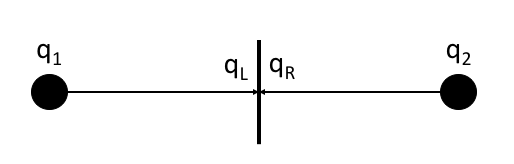
\includegraphics[width=0.5\textwidth]{figures/edge_reconstruction.png}
  \caption{Edge reconstruction.}
  \label{fig:edge-recons}
\end{figure}
%------------------------------------------------------------------------------%
The variable $\phi$ is the result of the scalar flux limiter function, that is
required to preserve monotonicity in the second order reconstruction near
discontinuities.  FUN3D supports a larger variety of flux limiters that fall
into two main categories: edge-based limiters, and stencil-based limiters.  The
edge based limiters are evaluated for two nodes at each edge.  Different values
of $\phi$ can exist at each node for edge-based limiter, and the results are not
``freezable'' at each node in FUN3D. Stencil-based limiters are evaluated at
each node, based on the gradients that are computed there.  For these limiters,
the value of $\phi$ is unique to each node and can be stored with the flow
solution as an additional variable.  The frozen state of the limiter is only
re-evaluated if the reconstruction forces a non-physical state at the dual
volume interface.

For this study, smooth Van Albada\cite{van1997comparative}, Van
Leer\cite{vatsa2009calibration}, and Minmod\cite{roe1986characteristic} flux
limiter functions are used.  Each of these limiters is augmented with a
heuristic pressure limiter by Park\cite{park2008anisotropic}. The choice of
these limiters impacts solution convergence and accuracy.  It is important to
note that the smooth Van Albada averaging function is given as
%------------------------------------------------------------------------------%
\begin{equation}
  \phi\left( a, b \right) =
  \frac{(b^2 + \varepsilon^2)a + (a^2 + \varepsilon^2)b}
  {a^2 + b^2 + 2\varepsilon^2}
  \label{van-albada-avg}
\end{equation}
%------------------------------------------------------------------------------%
where $a$ and $b$ are the left and right node gradients, and $\varepsilon$ is
the ``smoothing coefficient''.  This smoothing coefficient is used to tune the
flux limiter to a variety of the problems, and it is advised to be the
reciprocal of the mean aerodynamic chord (MAC) in grid units for
FUN3D\cite{biedron2016fun3d}.  The choice of $\varepsilon$ is critical to some
hypersonic applications involving chemistry, and will be discussed later.


\chapter{Design Optimization}
\label{chapter-four}

Design optimization is a wide field that encompasses methods generally falling into
two categories: local gradient-based optimization, and heuristic global
optimization.  Local gradient-based optimization techniques focus on the
determining an optimality condition by evaluating a function and its gradients.
Provided certain conditions are met, it can be proven that the optimization
procedure will find a local minimum or maximum on a bounded domain.  Examples of
local gradient-based optimization methods include steepest-descent[cite??],
conjugate-gradient[cite??], and Augmented Lagrangian Method [cite??].  A
heuristic global optimization seeks to find the global extrema of a function.
Although these methods are powerful, because of their heuristic nature they are
not guaranteed to find the absolute optimum condition and are not the focus this
research.

In the field of optimization, the function of interest is referred to as the
``cost function'' or ``objective function''.  Optimization methods seek to
minimize this function; therefore, if the intent is to find the maximum value
of the function, it should be formulated as the negative of the original.  This
section focuses on the implementation of the cost function components and design
variables used in the optimization, as well as the implementation of the
optimizer that is used.

\section{Cost Function Definition}

The cost function (or objective function) as formulated in FUN3D is a composite,
weighted function
%------------------------------------------------------------------------------%
\begin{equation}
  f = \sum_{j=1}^{N_{func}}w_j\left( C_j - C_{j^*} \right)^{p_j}
  \label{generic-cost-function}
\end{equation}
%------------------------------------------------------------------------------%
Where $w_j$, $C_{j^*}$, and $p_j$ are the weight, target, and power of cost
function component $j$.  $C_j$ is the component value, which is evaluated at
each flow solution.  For this particular optimization problem the cost function
is defined as 
%------------------------------------------------------------------------------%
\begin{equation}
  f = w_1\left( T_{RMS} \right)^{2} + w_2\left( C_{D} - C_{D}^{*} \right)^2
  \label{cd-tt-cost-function}
\end{equation}
%------------------------------------------------------------------------------%
The component weights were determined heuristically, to normalize the changes in
drag coefficient, $C_D$, and surface temperature Root-Mean-Square (RMS) $T_{RMS}$.
The drag coefficient is defined as
%------------------------------------------------------------------------------%
\begin{equation}
  C_D = \sum_{i}^{N_{faces}}
        \frac{2\left( p_i - p_\infty \right)n_{x_{i}}}
        {\rho_{\infty} V_{\infty}S_{ref}}
  \label{drag-coef-def}
\end{equation}
%------------------------------------------------------------------------------%
where $p_i$ is the average pressure at face $i$.  RMS of surface temperature is
defined as
\begin{equation}
  \sqrt{
    \frac{\sum_{i}^{N_{faces}}\left( T_{RMS} A_i \right)^2}
       {\sum_{i}^{N_{faces}}\left( A_i \right)^2}
     }
  \label{tt-rms-def}
\end{equation}
The area-weighted RMS of surface temperature was chosen over a simple
area-weighted average of surface temperature, because the stagnation temperature
is generally much higher than temperature elsewhere on a vehicle forebody in
hypersonic flows.  The squaring of temperature in the RMS will therefore give
greater weight to the stagnation temperature in the design.





\chapter{Demonstration Problem: Hypersonic Retro-firing Annular Jet}
\label{chapter-five}

To demonstrate the advantages and the robustness of the decoupled flow and
adjoint solvers relative to the fully coupled flow and adjoint solvers, a
demonstration problem is chosen with sufficiently challenging physics.  The
problem must include a sufficient sensitivity to the chemistry model to
highlight the stability concerns of the decoupled flow solver presented in
\sref{sec:15-kps-sphere-cone}.  In this case, the sensitivity manifests through
the formation of a large, recirculating buffer gas zone that covers most of the
vehicle outer surface. This chapter details the geometry and test conditions of
the demonstration problem, as well as the characteristics of the flow solution.

\section{Annular Jet Configuration and Test Conditions}

The geometry chosen is a hypersonic re-entry vehicle with a retro-firing annular
nozzle, as shown in \fref{fig:annular-jet-side}.
%------------------------------------------------------------------------------%
\begin{figure}[h]
  \centering
	\begin{subfigure}[b]{0.4\textwidth}
    \centering
    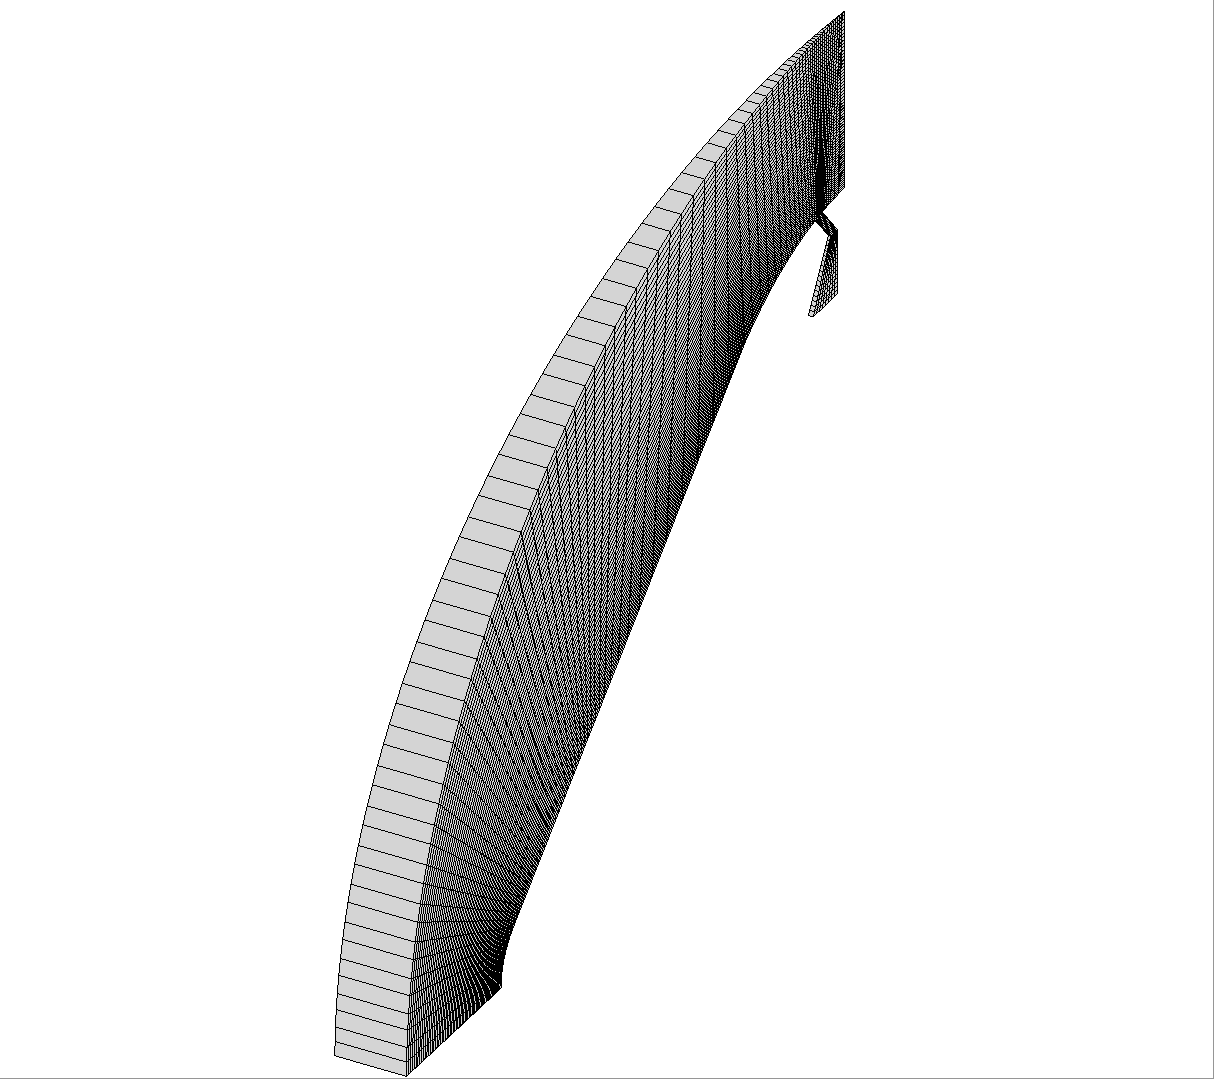
\includegraphics[width=\textwidth]{figures/iso-coarse.png}
  \end{subfigure}
	\begin{subfigure}[b]{0.4\textwidth}
    \centering
    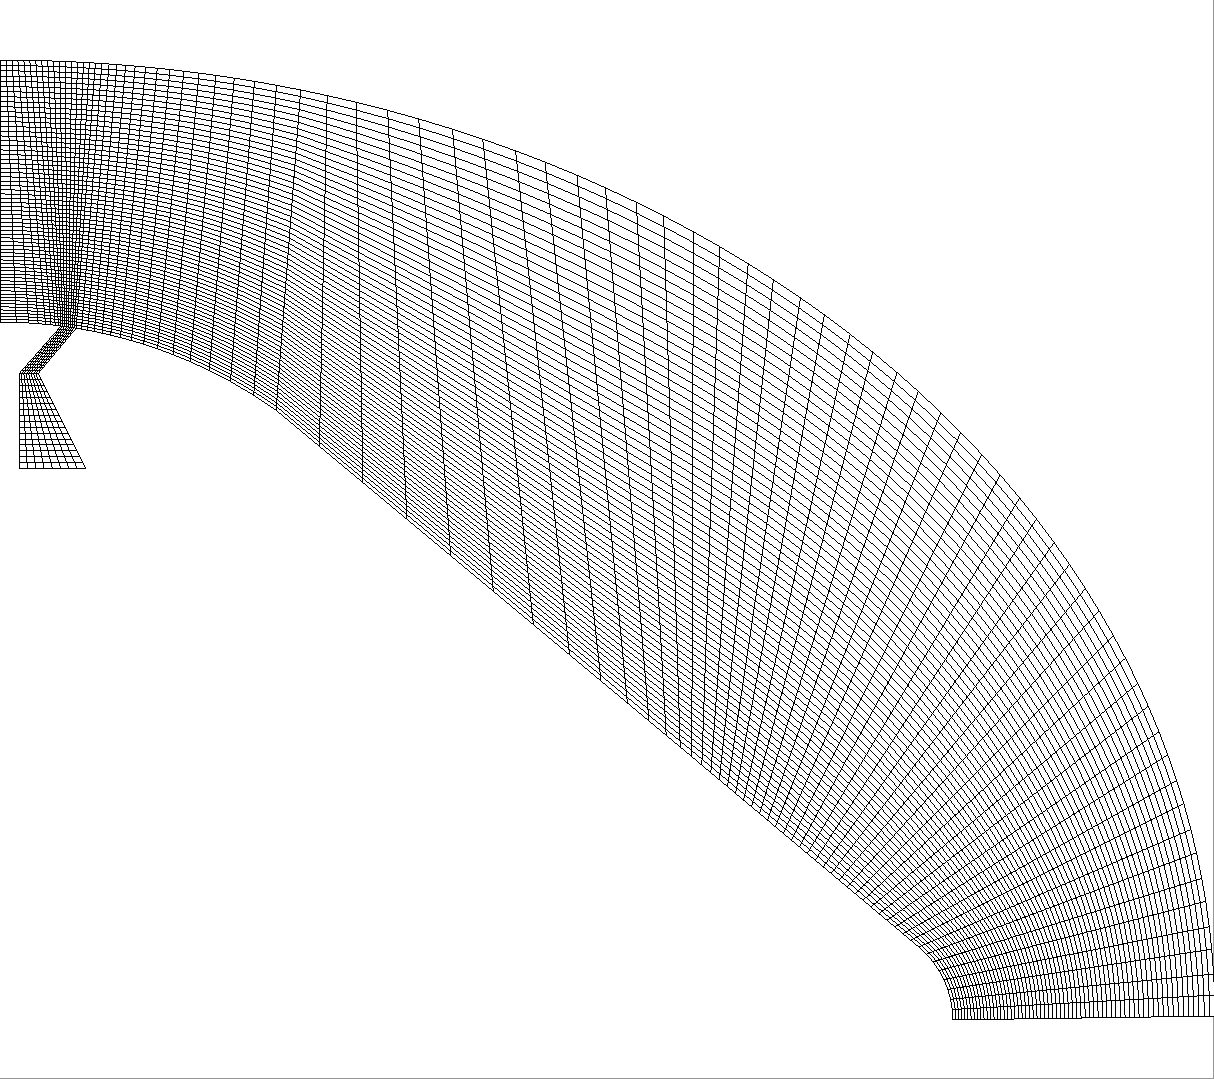
\includegraphics[width=\textwidth]{figures/side-coarse.png}
  \end{subfigure}
  \caption{Annular jet geometry.}
  \label{fig:annular-jet-side}
\end{figure}
%------------------------------------------------------------------------------%
This geometry was originally investigated by Gnoffo et
al\cite{gnoffo2016tapping} to obtain increased drag from ``pulsing'' the annular
jet to obtain a beneficial effect from the unsteady shock interaction with the
plume of the jet.  It was also determined from the aforementioned work that a
steady solution to the Euler equations exists for this annular jet
configuration.  This problem is attractive for optimization, because the annular
jet plenum conditions significantly affect aerodynamic and aerothermodynamic
quantities of interest on the vehicle surface.  These effects are very
non-linear, due to the shock and jet plume interaction, and it is therefore very
difficult to intuitively understand the relationship between the plenum
conditions and vehicle surface quantities.  Because the adjoint solver is
rigorously derived from the discretized governing equations, the relationship
between the plenum and surface can be directly determined, making this an
excellent showcase problem for adjoint-based sensitivity information.

%------------------------------------------------------------------------------%
\begin{table}[h]
  \centering
  \begin{tabular}{c|c|c}
    Parameter & Description & Value \\
    \hline
    $r_{throat}$       &   nozzle throat radius, $m$                 & 0.02 \\
    $r_{plenum,inner}$ &   inside nozzle radius at plenum face, $m$  & 0.02 \\
    $r_{plenum,outer}$ &   outside nozzle radius at plenum face, $m$ & 0.07 \\
    $r_{exit,inner}$   &   inside nozzle radius at exit, $m$         & 0.064 \\
    $r_{exit,outer}$   &   outside nozzle radius at exit, $m$        & 0.08 \\
    $l_{conv}$         &   distance from plenum to throat, $m$       & 0.05 \\
    $\theta_c$         &   cone half angle, deg                      & 50.0
  \end{tabular}
  \caption{Annular nozzle geometry inputs.}
  \label{tab:annular-geom}
\end{table}
%------------------------------------------------------------------------------%
The geometry was generated with the parameters shown in \tref{tab:annular-geom},
with the mesh originally created as structured grid and then converted to an
unstructured grid comprised of hexahedra and prismatic elements.  The flow
conditions for a Mach 20 condition are shown in \tref{tab:flow-conditions}, with
all simulations conducted using a 9-species Hydrogen-air mixture comprised of
$H_2$, $N_2$, $O_2$, $H$, $N$, $O$, $NO$, $OH$, and $H_2 O$.
%------------------------------------------------------------------------------%
\begin{table}[!h]
  \centering
  \begin{tabular}{c|c|c}
    Flow Condition & Description & Value \\
    \hline
    $V_{\infty}$    & freestream velocity, $m/s$        & 5686.24 \\
    $\rho_{\infty}$ & freestream density, $kg/m^3$      & 0.001 \\
    $T_{\infty}$    & freestream temperature, $K$       & 200.0 \\
    $M_{\infty}$    & freestream Mach number (derived)  & 20.0
  \end{tabular}
  \caption{Flow conditions.}
  \label{tab:flow-conditions}
\end{table}
%------------------------------------------------------------------------------%

\section{Annular Jet Flow Features and Steadiness Dependence on Cone Angle}

\frefs{fig:cone-angle-temperature}{fig:cone-angle-water} show contours for
annular plenum blowing pure hydrogen at 200,000 $Pa$ and 500$K$, and illustrate the
complexity of the physics associated with this annular jet configuration.  The
temperature contours in \fref{fig:cone-angle-temperature} show that the annular
jet configuration creates a buffer gas region behind the bow shock.  This buffer
gas provides a beneficial cooling mechanism for the outer surface of the
vehicle.  The production of water can be seen in \fref{fig:cone-angle-water},
with the overlayed streamlines indicating that a separation bubble forms just
downstream of the annular nozzle exit.  The degree of separation in this flow is
sensitive to the cone angle of the vehicle, and it has been observed that
lowering the cone angle reduces the size of this separation bubble.
%------------------------------------------------------------------------------%
\begin{figure}[h!]
  \centering
  \begin{subfigure}{0.45\textwidth}
    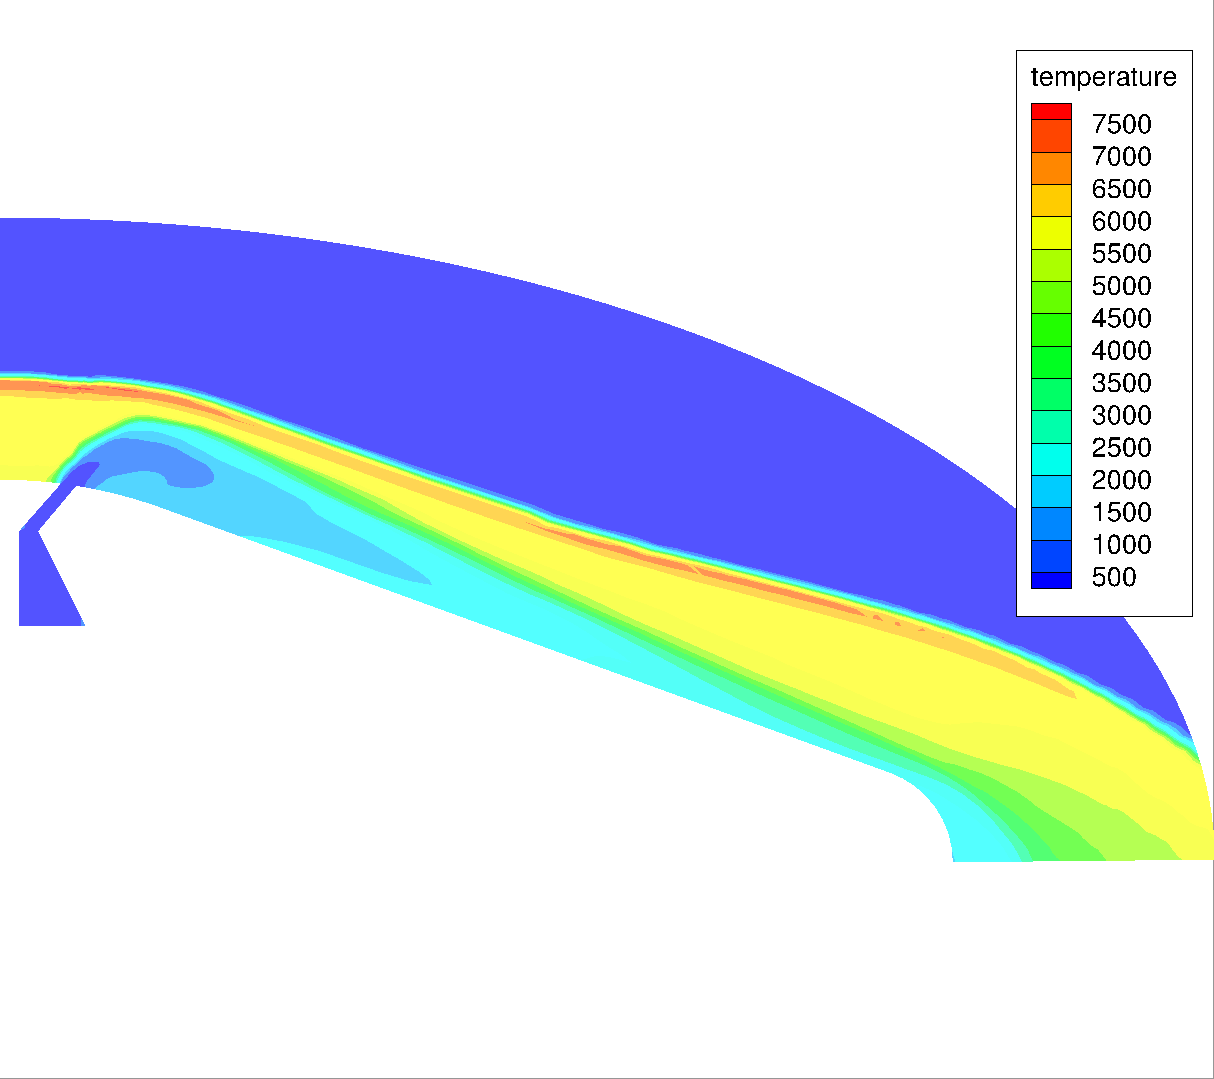
\includegraphics[width=\textwidth]{figures/srp/70deg-temperature.png}
    \caption{$70^o$ Cone angle}
    \label{fig:70deg-temperature-contour}
  \end{subfigure}
  \begin{subfigure}{0.45\textwidth}
    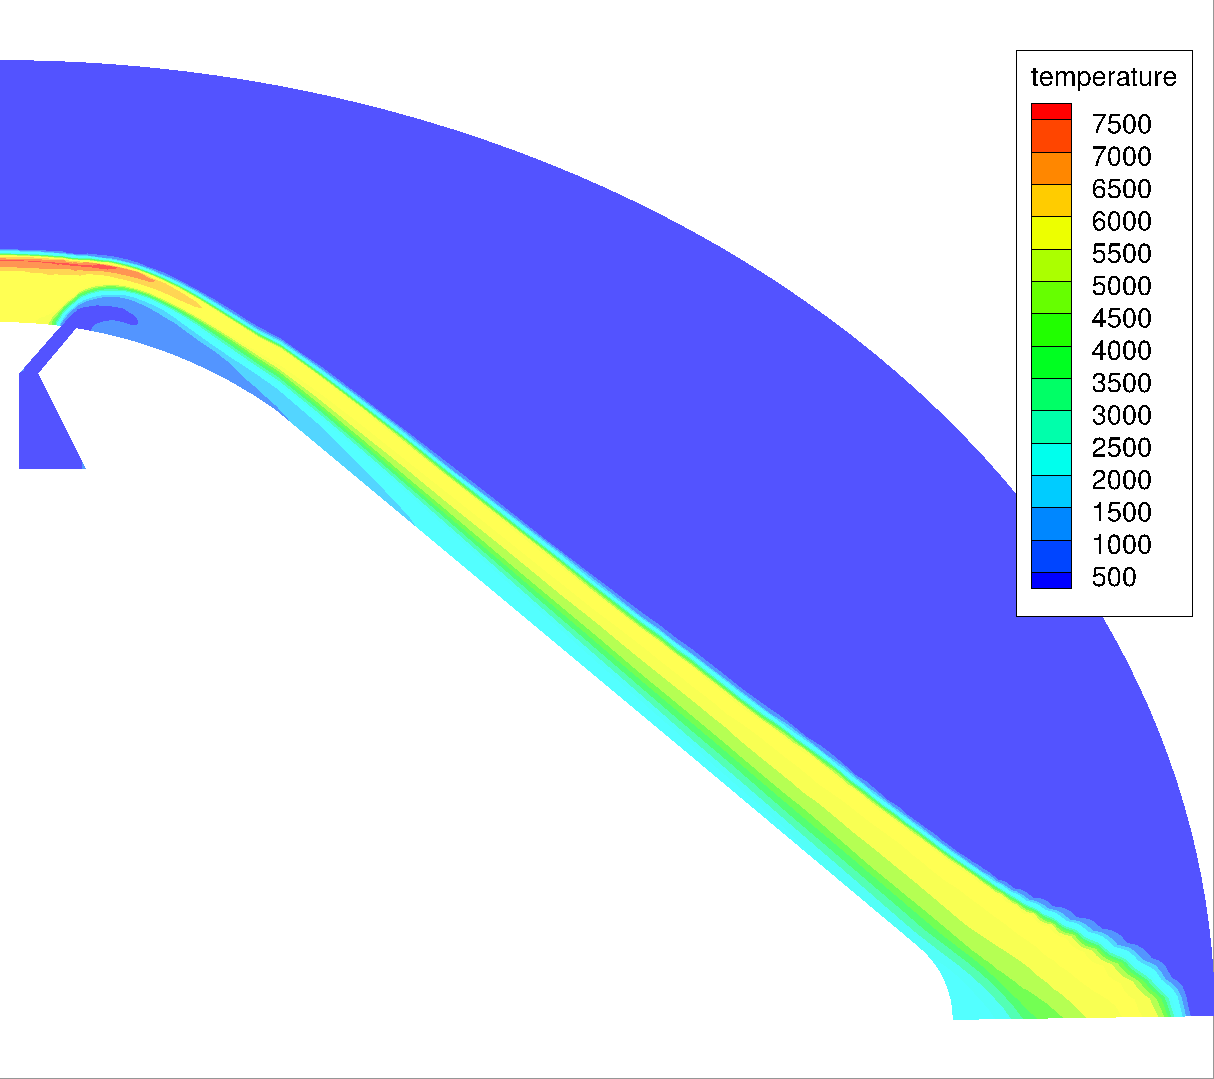
\includegraphics[width=\textwidth]{figures/srp/50deg-temperature.png}
    \caption{$50^o$ Cone angle}
    \label{fig:50deg-temperature-contour}
  \end{subfigure}
  \caption{Annular jet temperature contours, blowing pure $H_2$.}
  \label{fig:cone-angle-temperature}
\end{figure}
%------------------------------------------------------------------------------%
%------------------------------------------------------------------------------%
\begin{figure}[h!]
  \centering
  \begin{subfigure}{0.45\textwidth}
    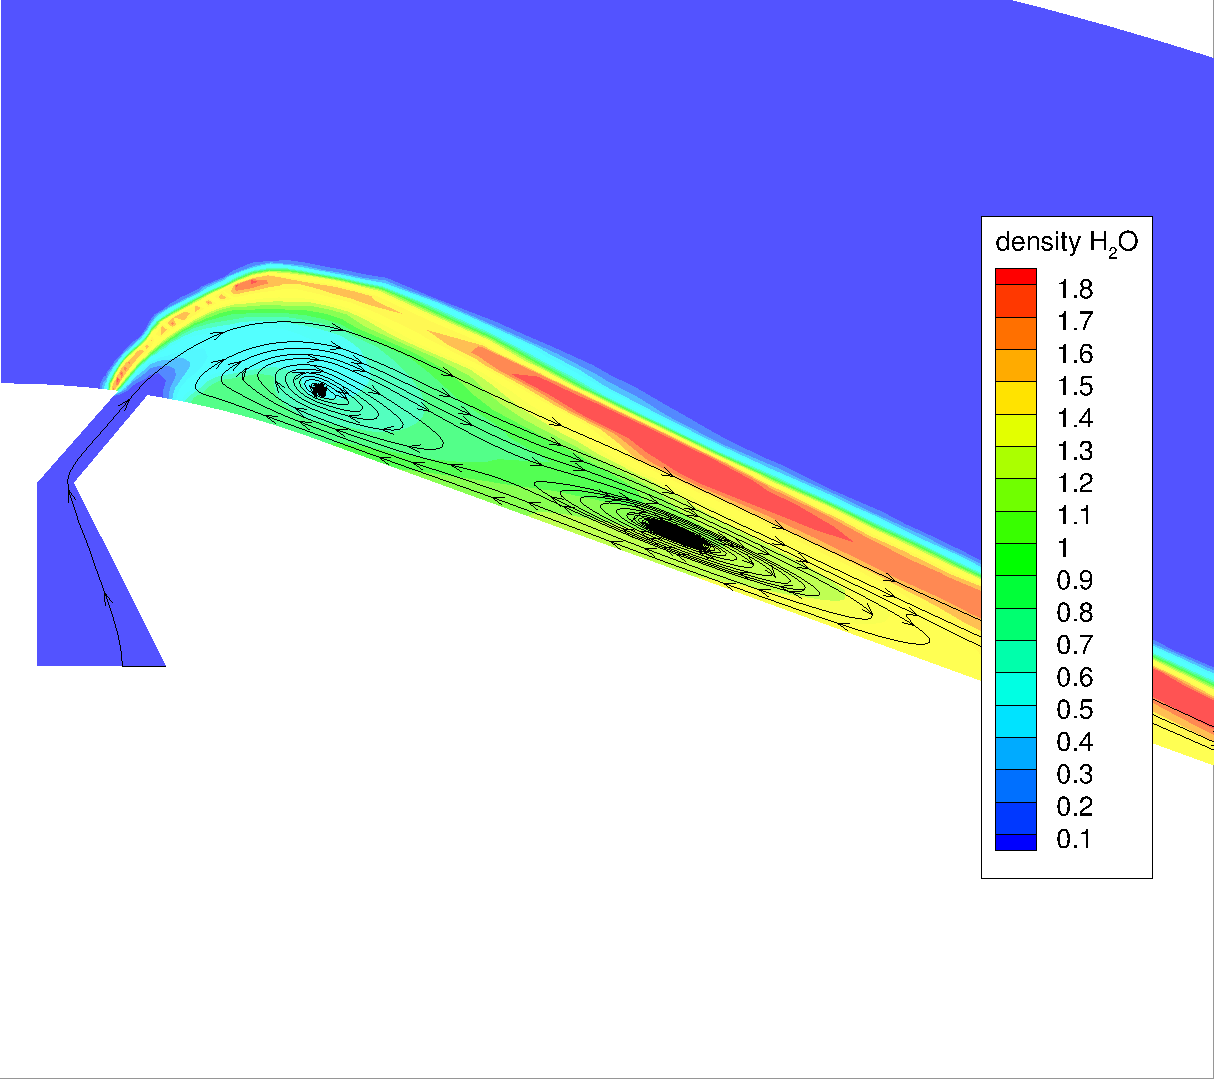
\includegraphics[width=\textwidth]{figures/srp/70deg-water.png}
    \caption{$70^o$ Cone angle}
    \label{fig:70deg-water-contour}
  \end{subfigure}
  \begin{subfigure}{0.45\textwidth}
    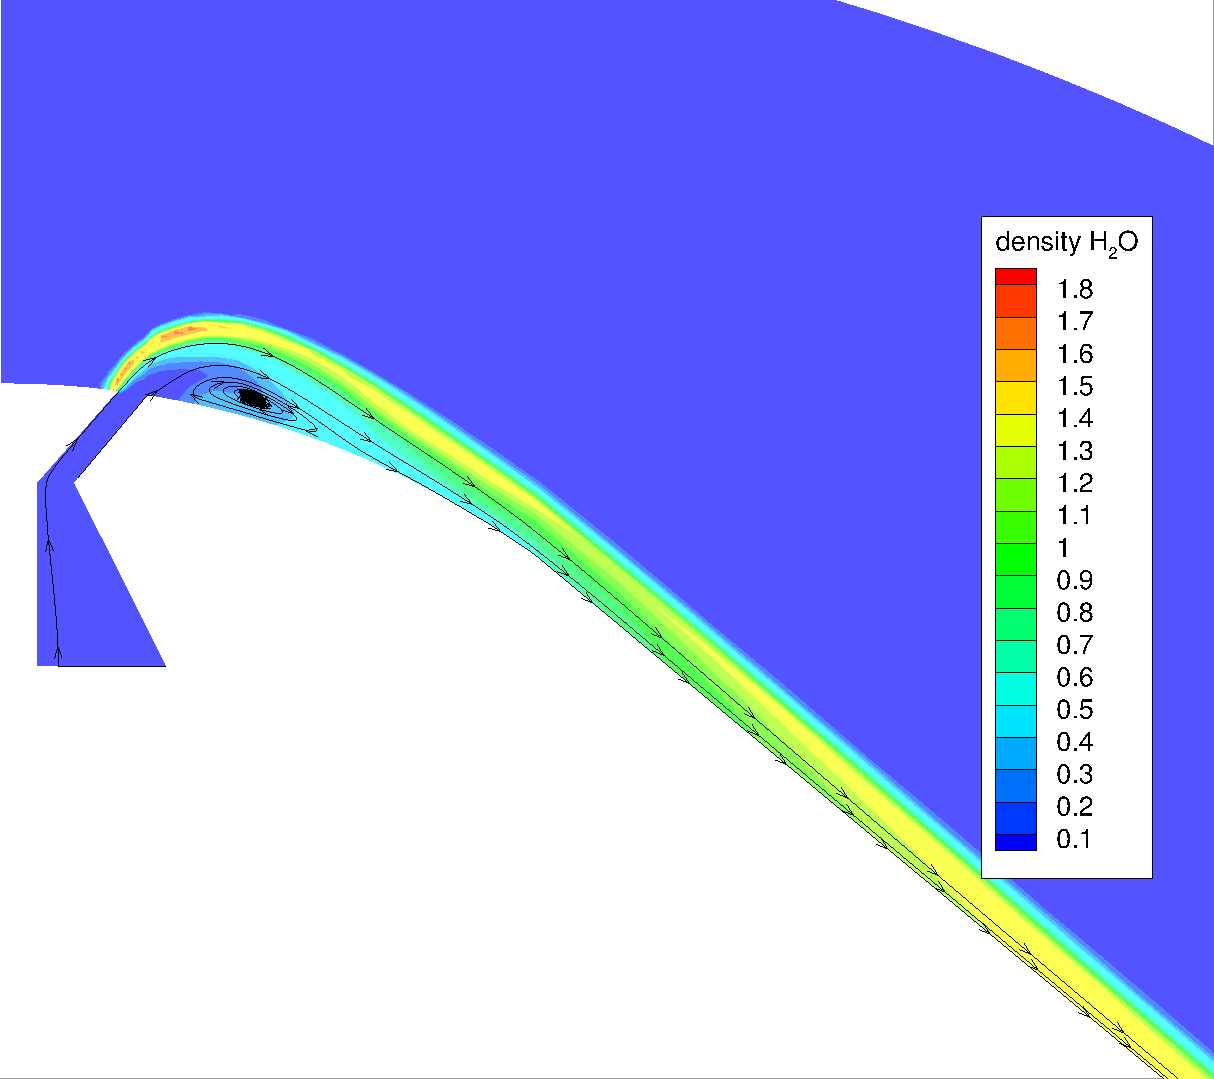
\includegraphics[width=\textwidth]{figures/srp/50deg-water.png}
    \caption{$50^o$ Cone angle}
    \label{fig:50deg-water-contour}
  \end{subfigure}
  \caption{Annular jet $H_2 O$ density contours, blowing pure $H_2$.}
  \label{fig:cone-angle-water}
\end{figure}
%------------------------------------------------------------------------------%

The size of the separation bubble shown in \fref{fig:cone-angle-water} has
implications on the steadiness of the flow.  While the reacting gas path of the
FUN3D flow solver has the capability to simulate unsteady flows, the newly
developed FUN3D reacting gas adjoint solver is currently limited in scope to
steady flows.  A full design optimization covers a wide variety of flow
solutions, and it is therefore important to verify that the geometry chosen
results in steady flow for all design perturbations.  A $70^o$ cone angle was
initially chosen, instead of $50^o$, because of a rich history of investigation
associated with the Mars Pathfinder probe\cite{gnoffo1996influence}.  It was
heuristically determined that blowing a light gas with a high cone angle leads
to a sonic corner body.  Numerical experiments indicate that the annular jet is
susceptible to very low frequency and low amplitude pulsing of the entrained
separation bubble on sonic corner bodies, where the separation bubble near the
nozzle exit is relatively large.
%------------------------------------------------------------------------------%
\begin{figure}[h]
  \centering
  \begin{subfigure}[b]{0.45\textwidth}
    \centering
    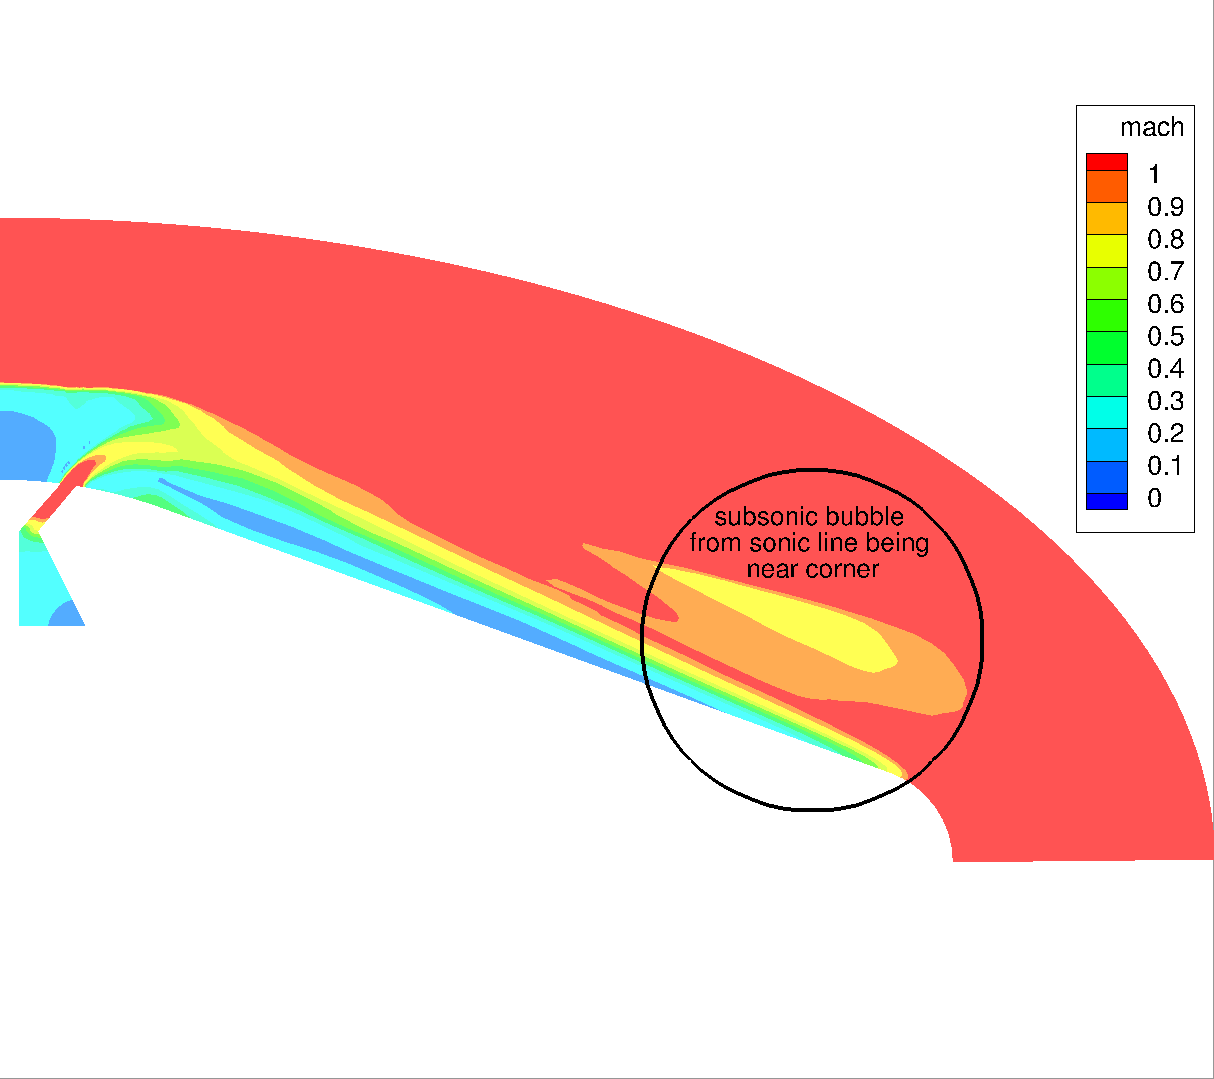
\includegraphics[width=\textwidth]{figures/sonic-bubble/sonic_bubble.png}
    \caption{$70^o$ Cone angle}
    \label{fig:70-deg-cone}
  \end{subfigure}
  \begin{subfigure}[b]{0.45\textwidth}
    \centering
    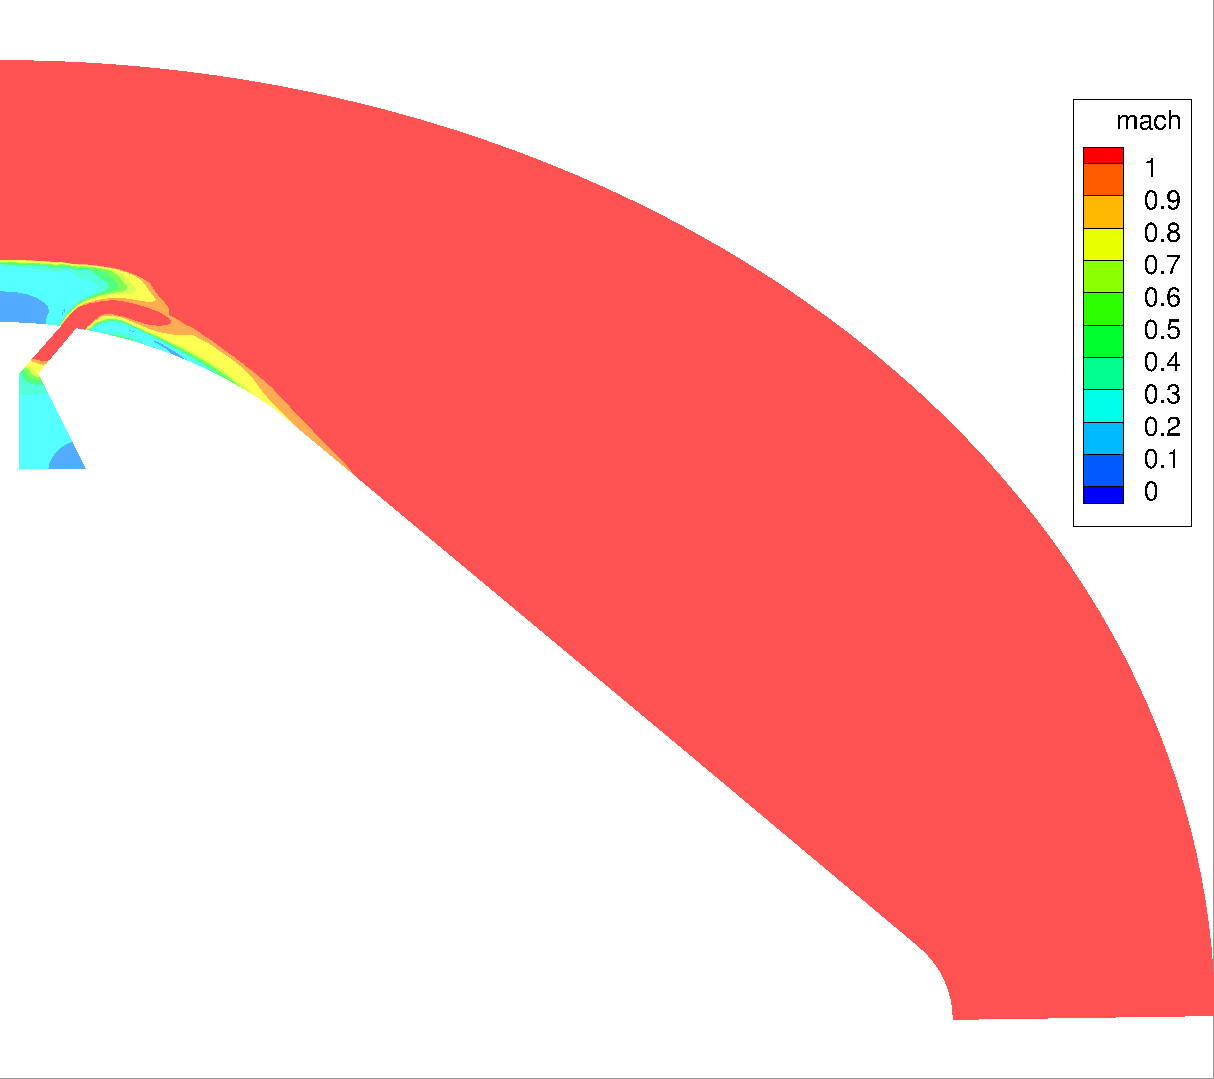
\includegraphics[width=\textwidth]{figures/sonic-bubble/no_bubble.png}
    \caption{$50^o$ Cone angle}
    \label{fig:50-deg-cone}
  \end{subfigure}
  \caption{Annular jet sonic line comparison, blowing pure $H_2$.}
  \label{fig:cone-angle-comp}
\end{figure}
%------------------------------------------------------------------------------%
\fref{fig:cone-angle-comp} shows a comparison of mach number for the same flow
conditions as those in \frefs{fig:cone-angle-temperature}{fig:cone-angle-water}.
\fref{fig:70-deg-cone} highlights the subsonic bubble that is indicative of a
sonic corner body, whereas \fref{fig:50-deg-cone} shows that decreasing the cone
angle moves the sonic line upstream and eliminates the subsonic bubble.  The
strong dependence between the position of the sonic line on the vehicle and the
cone angle is the primary reason that the cone angle was chosen to be decreased
to $50^o$, rather that using the $70^o$ chosen by Gnoffo et
al.\cite{gnoffo2016tapping}.  The comparison between the $50^o$ and $70^o$ cone
angle geometries was done for a wide range of plenum conditions spanning the
design space to be discussed in the next chapter, and no subsonic bubble was
ever found for the $50^o$ cone angle.

\section{Mesh Refinement Study}
\label{sec:mesh-refinement-study}

To determine the flow solution mesh sensitivity, a grid convergence study was
attempted by uniformly refining the original mesh, using the cut-cell method
developed by Park\cite{park2008anisotropic} that uniformly subdivides each
element in the mesh.
%------------------------------------------------------------------------------%
\begin{table}[h]
  \centering
  \begin{tabular}{c|c}
    Plenum Condition & Value \\
    \hline
    Plenum Pressure, $P_{p,o}$, Pa   & 200,000 \\
    Plenum Temperature, $T_{p,o}$, K &  500 \\
    Plenum Fuel-Air Ratio $\fa$      &  0.7
  \end{tabular}
  \caption{Plenum conditions.}
  \label{tab:plenum-conditions}
\end{table}
%------------------------------------------------------------------------------%
The solution on each grid level was computed using the freestream conditions in
\tref{tab:flow-conditions} and the plenum conditions in
\tref{tab:plenum-conditions}, and \fref{fig:mesh-refined} shows the progression
of refined meshes generated by this method,
%------------------------------------------------------------------------------%
\begin{figure}[h]
  \centering
  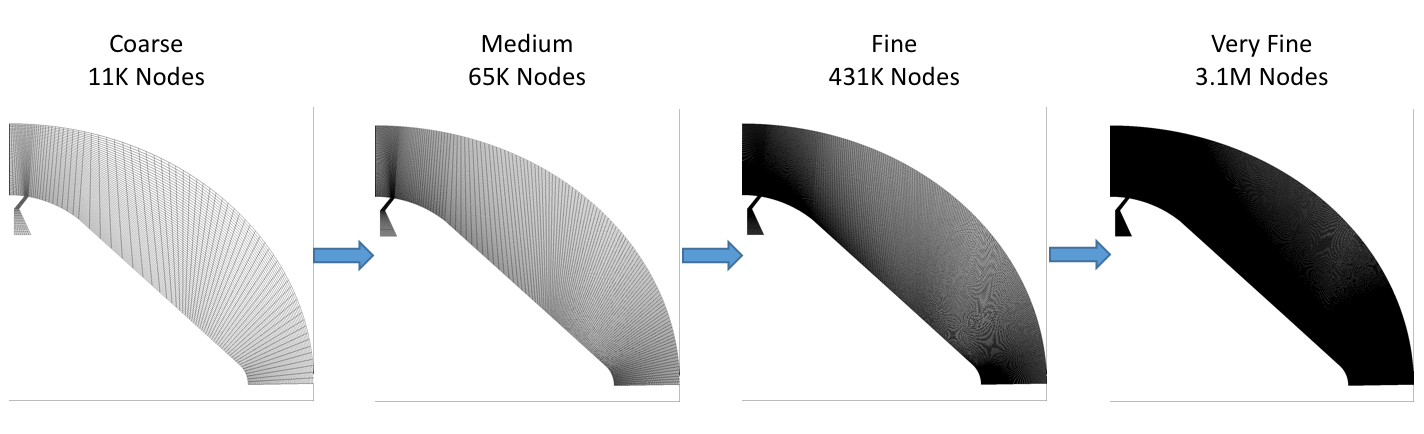
\includegraphics[width=\textwidth]{figures/mesh-progression.png}
  \caption{Uniformly refined meshes.}
  \label{fig:mesh-refined}
\end{figure}
%------------------------------------------------------------------------------%
and \fref{fig:grid-convergence} shows the grid convergence of surface
temperature and plenum mass flow rate for a nominal case.
%------------------------------------------------------------------------------%
\begin{figure}[!h]
  \centering
  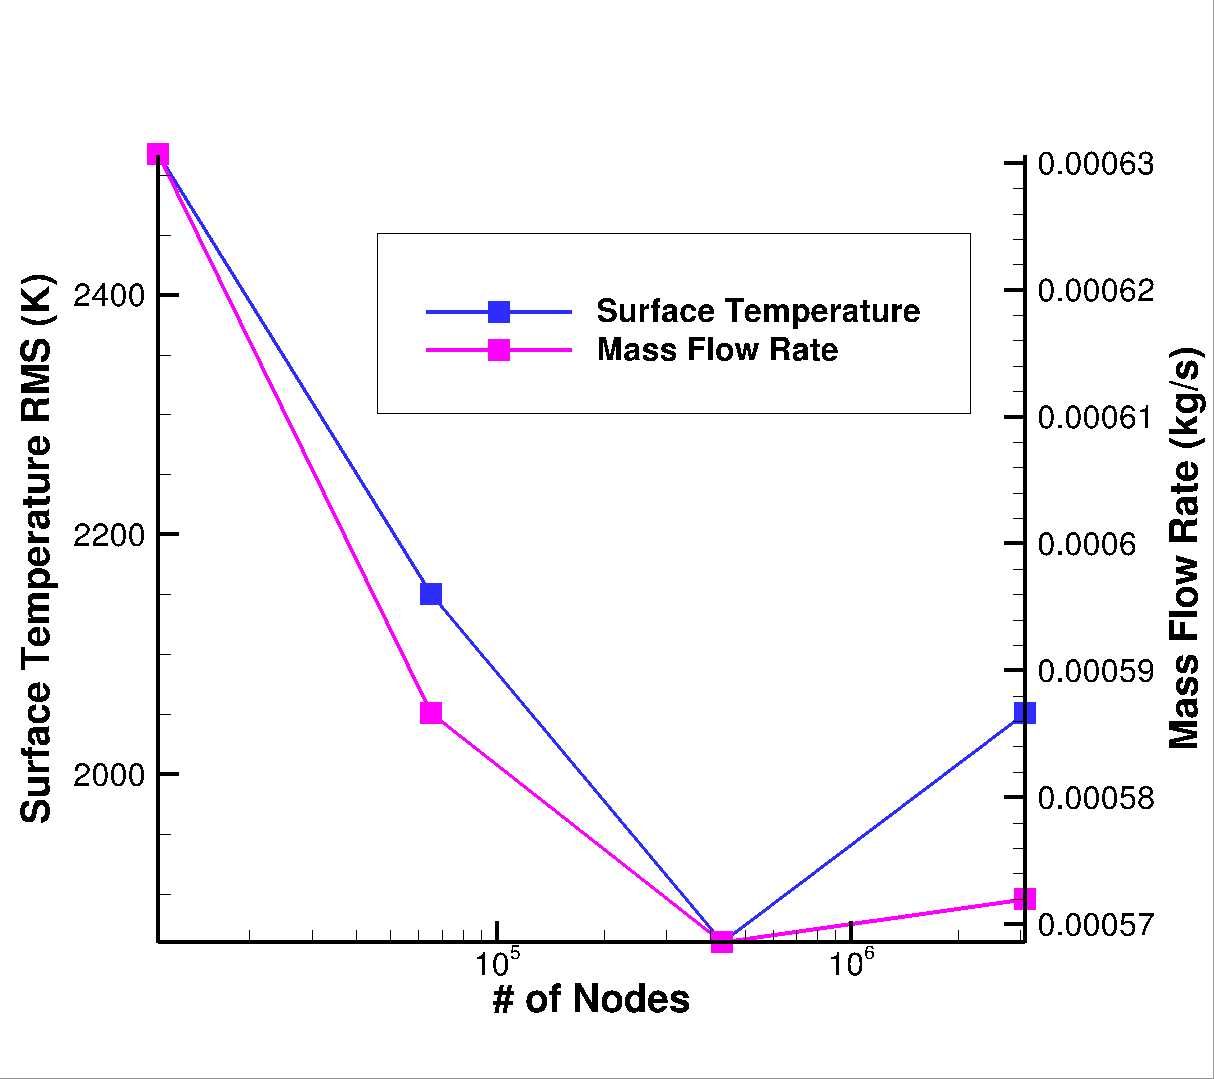
\includegraphics[width=0.5\textwidth]{figures/t-m-conv.png}
  \caption{Grid convergence.}
  \label{fig:grid-convergence}
\end{figure}
%------------------------------------------------------------------------------%
On the fine mesh ($431,000$ Nodes), a frozen limiter was required to maintain
stead flow.  The flow solution for the very fine mesh ($3,100,000$ Nodes) was
very unsteady, and freezing the flux limiter did not recover a steady flow
solution.  The values for surface temperature and mass flow rate on the very
fine mesh are time averaged quantities presented for qualitative purposes only.
This grid convergence study shows that the demonstration problem enables
unsteadiness on the finest mesh.  For the purposes of demonstrating the
decoupled discrete adjoint, the discretized flow solution must remain steady;
therefore, the coarse mesh ($11,000$ nodes) is used as a baseline for the
remainder of this study.  The adjoint formulation only requires steady flow on
the given grid; therefore, this test retains all of the challenging interaction
associated with a large, recirculating buffer zone over the cone with a strong
dependence on the reacting gas physics.

\section{Sensitivity to Frozen Flux Limiter}
\label{sec:frozen-limiter}

The use of a flux limiter is mandatory to maintain monotonicity in hypersonic
applications, where strong shocks are present; however, the solver is very
sensitive to changes in the reconstruction, and a ``ringing'' of the residual is
often observed\cite{gnoffo2007ringing} when using a flux limiter in FUN3D. While
this sub-convergence of the flow equation residuals is not detrimental to the
flow solver results, as most aerothermodynamic quantities are usually
sufficiently converged by this point, the adjoint-formulation is predicated on
the residual being machine zero.  Because of this last point, the stalled
convergence can cause the adjoint solver to give incorrect results or cause the
adjoint solution to diverge.  To prevent this divergence, the adjoint is
required to be run with a ``frozen'' limiter, where a limiter value is only
updated and re-frozen where a reconstruction is unrealisable using the current
limiter value.  Freezing the limiter in this way usually results in the
residuals converging to machine precision.

A particular difficulty of this approach comes from simulations on
shock-misaligned meshes involving chemical reactions.  Because the annular jet
plume and bow shock cannot remain aligned with the mesh during a design
optimization, there is a larger degree of ringing as the scheme captures the
discontinuities of these flow phenomena.  The ringing is mitigated when the
limiter is frozen; however, the solution will experience high-frequency errors
as the shock and plume re-position due to the reconstruction changing somewhat
asymmetrically.  Species will quickly deplete and form as the shock and plume
move, potentially requiring further reevaluation of the flux limiter at those
nodes.  This process will eventually settle out, and the flow solution will
converge to machine zero, with the definition of machine zero being dependent on
the conditioning of the problem being solved.  
%------------------------------------------------------------------------------%
\begin{figure}[h]
  \centering
  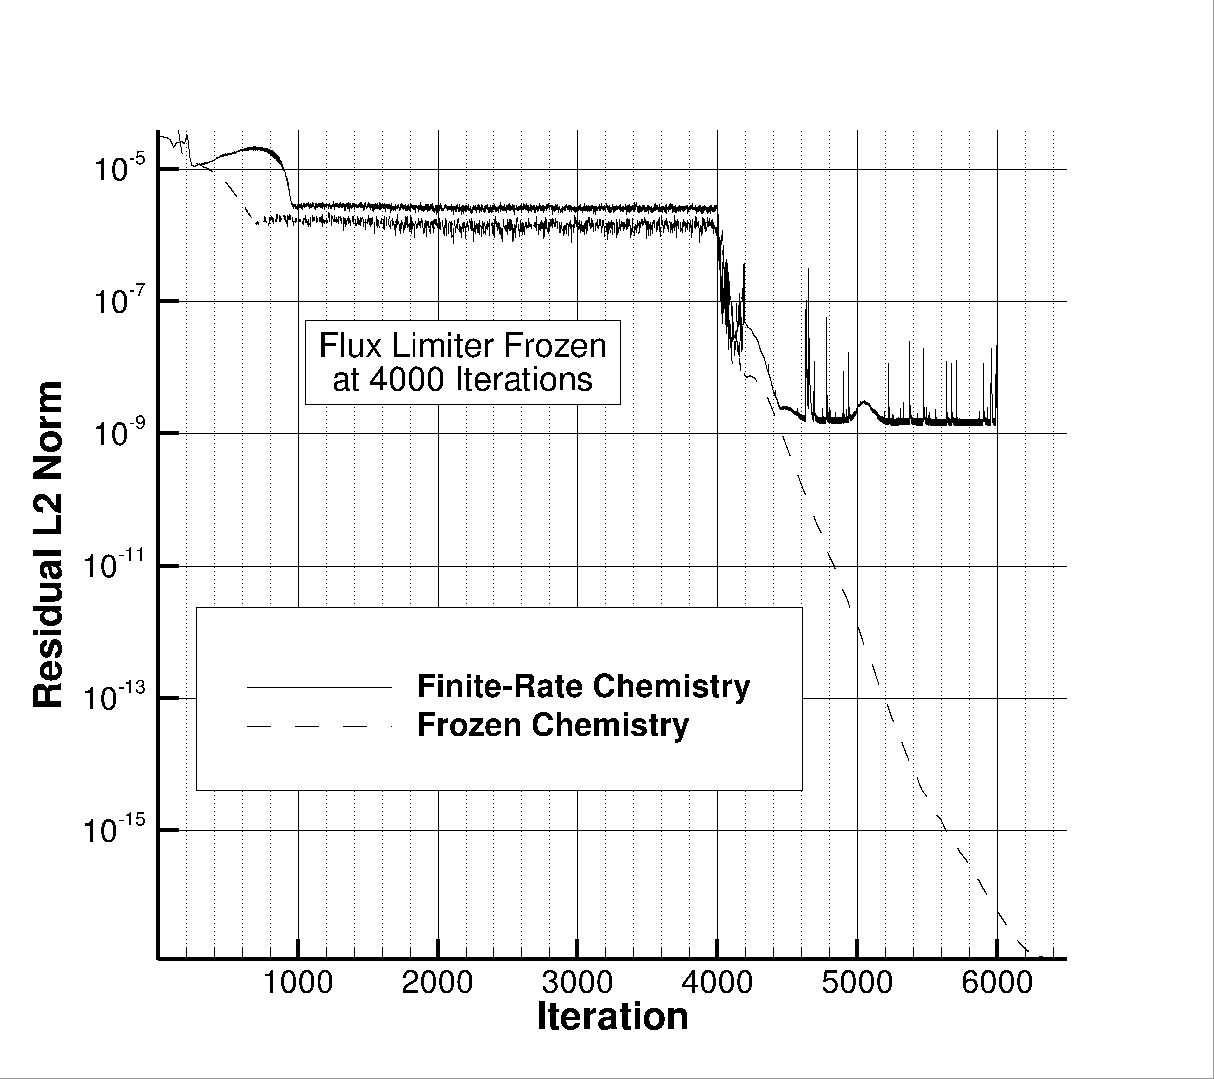
\includegraphics[width=0.5\textwidth]{figures/limiters/chem-res-comp.png}
  \caption{Typical residual convergence behavior.}
  \label{fig:chem-res-comp}
\end{figure}
%------------------------------------------------------------------------------%
\fref{fig:chem-res-comp} shows a typical convergence history for the annular jet
case with a flux limiter engaged on the coarse mesh.  If no chemical reactions
are allows to take place, i.e. ``frozen'' flow, the residual of all equations
can be decreased to to less than $10^{-16}$.  If finite rate chemistry is
included, convergence ends at $\sim 10^{-8}$.  The difference is believed to be
associated with the high degree of stiffness in the chemical source terms.  The
large reaction rates significantly increase the condition number of the
Jacobian, and further updates to the solution do not improve convergence.  This
is not a problem for the adjoint solution, as both levels of convergence are
sufficient to obtain an adjoint solution; however, the convergence of the flow
equations with chemistry is marred by the high degree of sensitivity to the flux
limiter used.  It can be seen in \fref{fig:chem-res-comp} that convergence
to
steady state is less smooth when chemistry is involved, and this is directly
tied to the flux limiter field.  In FUN3D, the frozen flux limiter is
re-evaluated when a reconstruction is unrealisable.  This reevaluation causes
high-frequency errors, which manifest as ``spikes'' in the residual history.
Fortunately, the reevaluation is only needed at a small number of nodes
(usually $< 10$ nodes), so integrated aerothermodynamic quantities are
unaffected by these reevaluations when convergence to steady-state is reached.
It should be noted that while the results presented here are only on the
coarsest (baseline) mesh level, the refined meshes also exhibit similar
behavior.

Because the solution is not grid converged, there is a significant difference
between the first-order and second-order solutions; therefore, the choice flux
limiters presented in \sref{sec:2nd-order-reconstruction} has a large impact on
the solution.  
%------------------------------------------------------------------------------%
\begin{figure}[h]
  \centering
  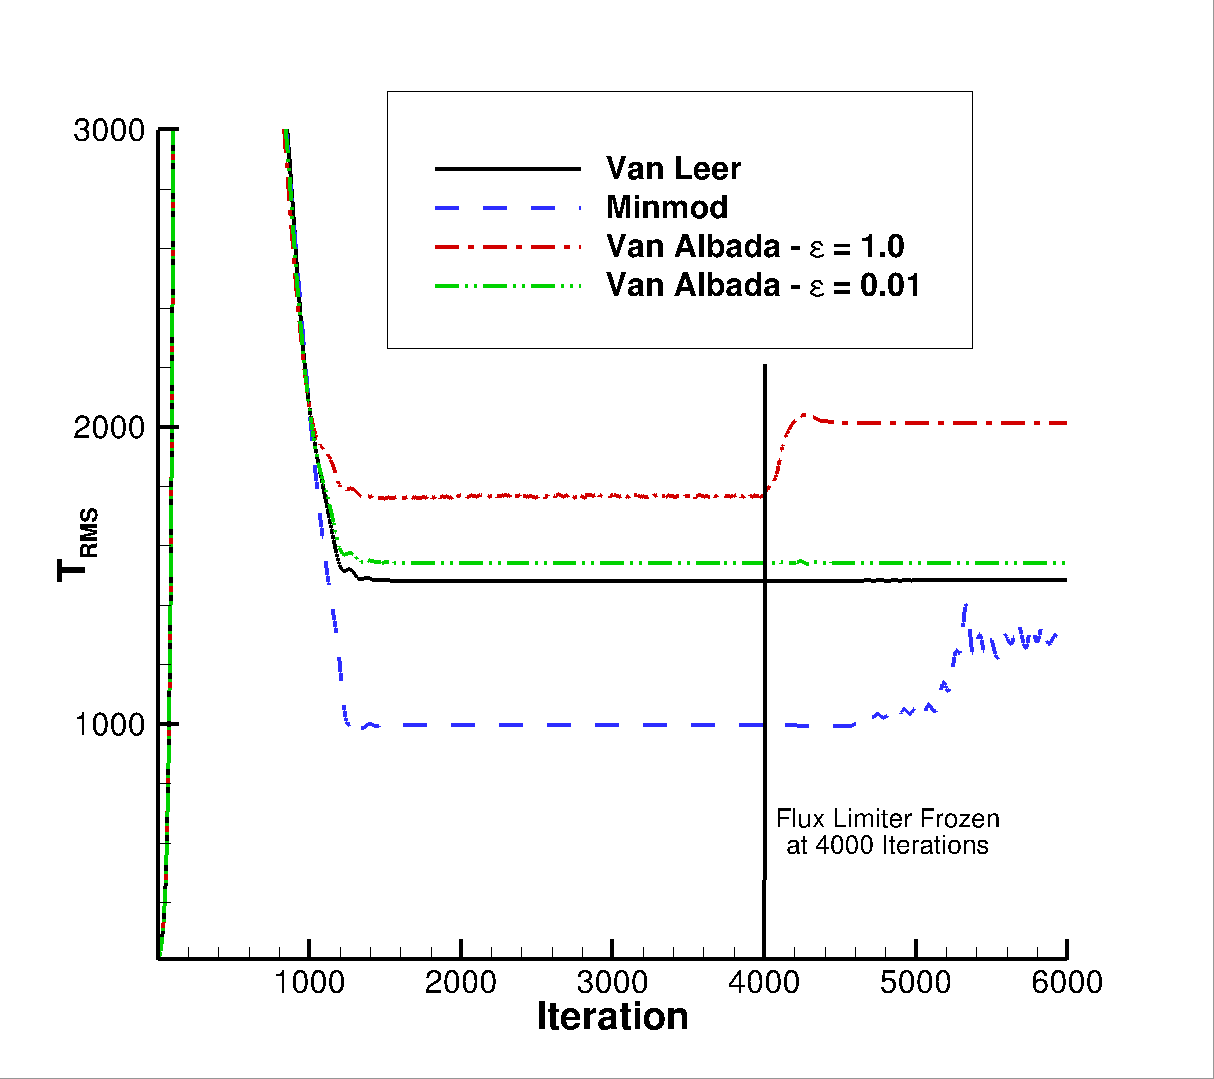
\includegraphics[width=0.5\textwidth]{figures/limiters/all-limiters.png}
  \caption{Convergence of surface temperature with different flux limiters.}
  \label{fig:all-limiters}
\end{figure}
%------------------------------------------------------------------------------%
\fref{fig:all-limiters} shows that the RMS of surface temperature on the outer
surface of the vehicle converges to significantly different results before
the flux limiter is frozen at iteration 4000.  The Minmod flux limiter exhibits
very large oscillations after freezing, due to the large number of non-smooth
reevaluations of the flux limiter were reconstructions became unrealisable.
These oscillations in the solution make the Minmod flux limiter unusable for
design optimization of this case. The Van Albada flux limiter converges to a
much more steady solution after being frozen; however, care must be taken to
``tune'' this particular limiter based the grid.  The tunable parameter,
$\varepsilon$, was evaluated at the recommended value of $1.0$, and was found to
increase the surface temperature by $> 20\%$ after freezing.  This is
unacceptable for design optimization, as it indicates a high dependence on
iteration that the flux limiter is frozen.
%------------------------------------------------------------------------------%
\begin{figure}[h]
  \centering
  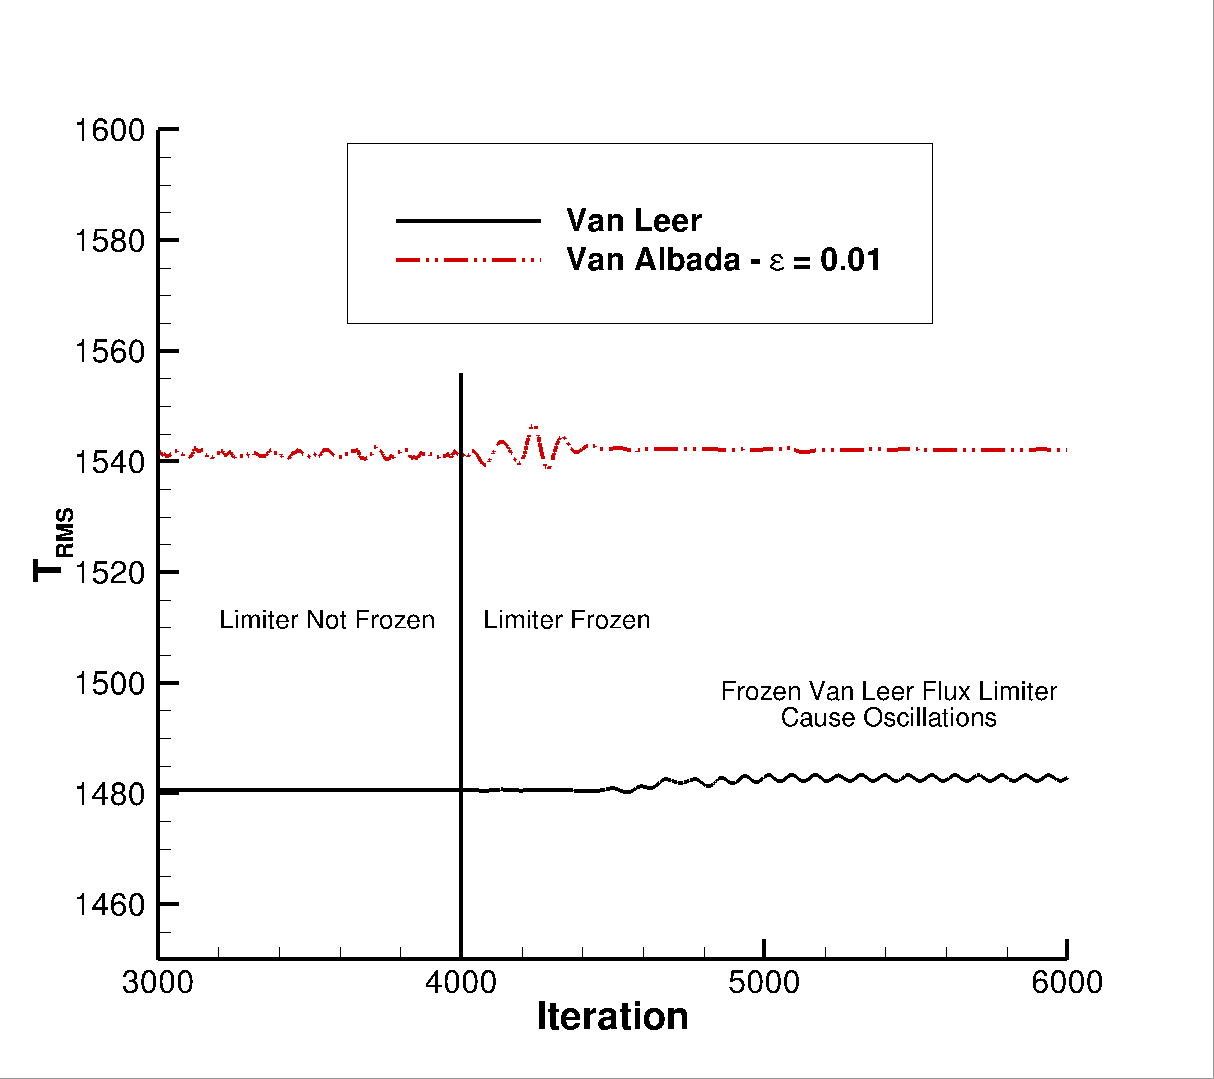
\includegraphics[width=0.5\textwidth]{figures/limiters/vanleer-vanalbada-frozen.png}
  \caption{Van Leer and Van Albada flux limiter impact on surface temperature.}
  \label{fig:vl-va-impact}
\end{figure}
%------------------------------------------------------------------------------%
The Van Leer flux limiter behaves much better in this regard; however,
\fref{fig:vl-va-impact} shows that the Van Leer limiter is also prone to
oscillations in the surface temperature RMS.  The oscillations are of small
enough amplitude that it might be reasonable to use the Van Leer flux limiter in
a design optimization of this problem, but a better alternative is to revisit
the Van Albada flux limiter.  \fref{fig:vl-va-impact} also shows that if
$\varepsilon$ is tuned to a value of $0.01$ the surface temperature RMS very
closely matches the average of the ringing value before the limiter was frozen.
For this reason, the Van Albada flux was used with $\varepsilon = 0.01$, which
tends towards the highly limited solution, as it seems to produce the most
steady result with the least dependence on the iteration that the flux limiter
is frozen.

None of the aforementioned flux limiter choices are ideal.  Because of the
sensitivity exhibited to freezing the limiter, integrated aerothermodynamic
quantities results can vary between solution with the same inputs, but different
starting states.  Tuning the Van Albada flux limiter mitigates this issue, but
does not solve it entirely, with some cases resulting in a surface temperature
RMS variance of $+/- 5 K$ with identical solver inputs but different flow
starting conditions. This is a recognized problem, but one that is outside of
the scope of this study.  A number of novel discretizations at at NASA Langley
Research Center\cite{gnoffo2014global,mazaheri2014very,mazaheri2016high} show
promise in mitigating or eliminating the need for a flux limiter, while
achieving higher-order spatial accuracy, and future work may incorporate them.

\chapter{Design Optimization}
\label{chapter-six}

Design optimization is a wide field that encompasses methods generally falling
into two categories: local gradient-based optimization, and heuristic global
optimization.  Local gradient-based optimization techniques focus on the
determining an optimality condition by evaluating a function and its gradients.
Provided certain conditions are met, it can be proven that the optimization
procedure will find a local minimum or maximum on a bounded domain.  Examples of
local gradient-based optimization methods include
steepest-descent\cite{fletcher1963rapidly}, sequential quadratic programming
(SQP)\cite{SNOPT-alg}, as well as an interesting method that converts a
constrained optimization problem into an unconstrained on by employing the
Kreisselmeier-Steinhauser function\cite{wrenn1989indirect}.  A heuristic global
optimization seeks to find the global extrema of a function.  Although these
methods are powerful, because of their heuristic nature they are not guaranteed
to find the absolute optimum condition and are not the focus this research.

In the field of optimization, the function of interest is referred to as the
``cost function'' or ``objective function''.  Optimization methods seek to
minimize this function; therefore, if the intent is to find the maximum value
of the function, it should be formulated as the negative of the original.  This
section focuses on geometry and test conditions for the optimization, the
implementation of the cost function components and design variables used in the
optimization, as well as the interface to the optimizer that is used.

\section{Integrated Quantities of Interest}

The primary objective of this optimization is to explore the effects of the plume
from the annular jet interacting with the bow shock.  Rather than focus on the
net force contribution of this annular jet geometry to drag, as was previously
investigated by Gnoffo et. al \cite{gnoffo2016tapping}, the primary objective of
this study is to efficiently cool the surface of the vehicle with minimal mass
added to the vehicle.  Since only inviscid flow was done in this study, and the
root-mean-square (RMS) of surface temperature is taken as an analog to the
surface heating rate.  Likewise, the massflow rate through nozzle plenum
boundary is taken as an analog to the addition of mass to the vehicle.

The RMS of surface temperature is defined as
%------------------------------------------------------------------------------%
\begin{equation}
  T_{RMS} =
  \sqrt{
    \frac{\sum_{i}^{N_{faces}}\left( T_{RMS} A_i \right)^2}
       {\sum_{i}^{N_{faces}}\left( A_i \right)^2}
     }
  \label{tt-rms-def}
\end{equation}
%------------------------------------------------------------------------------%
The area-weighted RMS of surface temperature was chosen over a simple
area-weighted average of surface temperature, because the temperatures on the
vehicle forebody are likely non-uniform, and there are regions of very high
temperature near the stagnation region of a vehicle forebody in hypersonic
flows.  Squaring of temperature in the RMS will give greater weight to the
these high-temperature regions in the design, as these are the in the most
danger of burn-through.
%------------------------------------------------------------------------------%
\begin{figure}[h]
  \centering
	\begin{subfigure}[b]{0.4\textwidth}
    \centering
    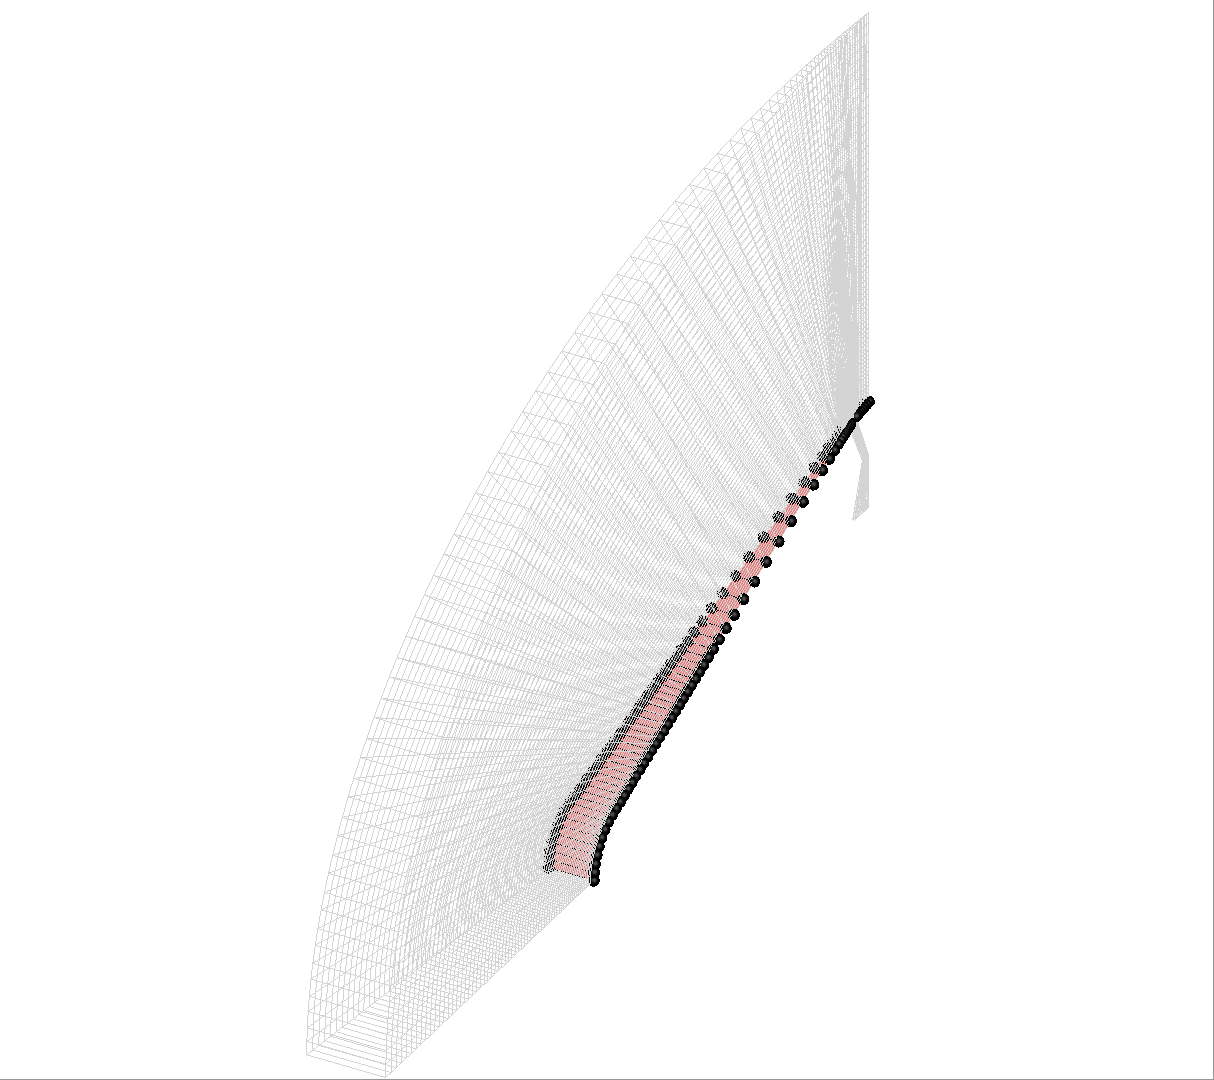
\includegraphics[width=\textwidth]{figures/surface2.png}
    \caption{$T_{RMS}$ Integrated Area}
    \label{fig:t-rms-area}
  \end{subfigure}
	\begin{subfigure}[b]{0.4\textwidth}
    \centering
    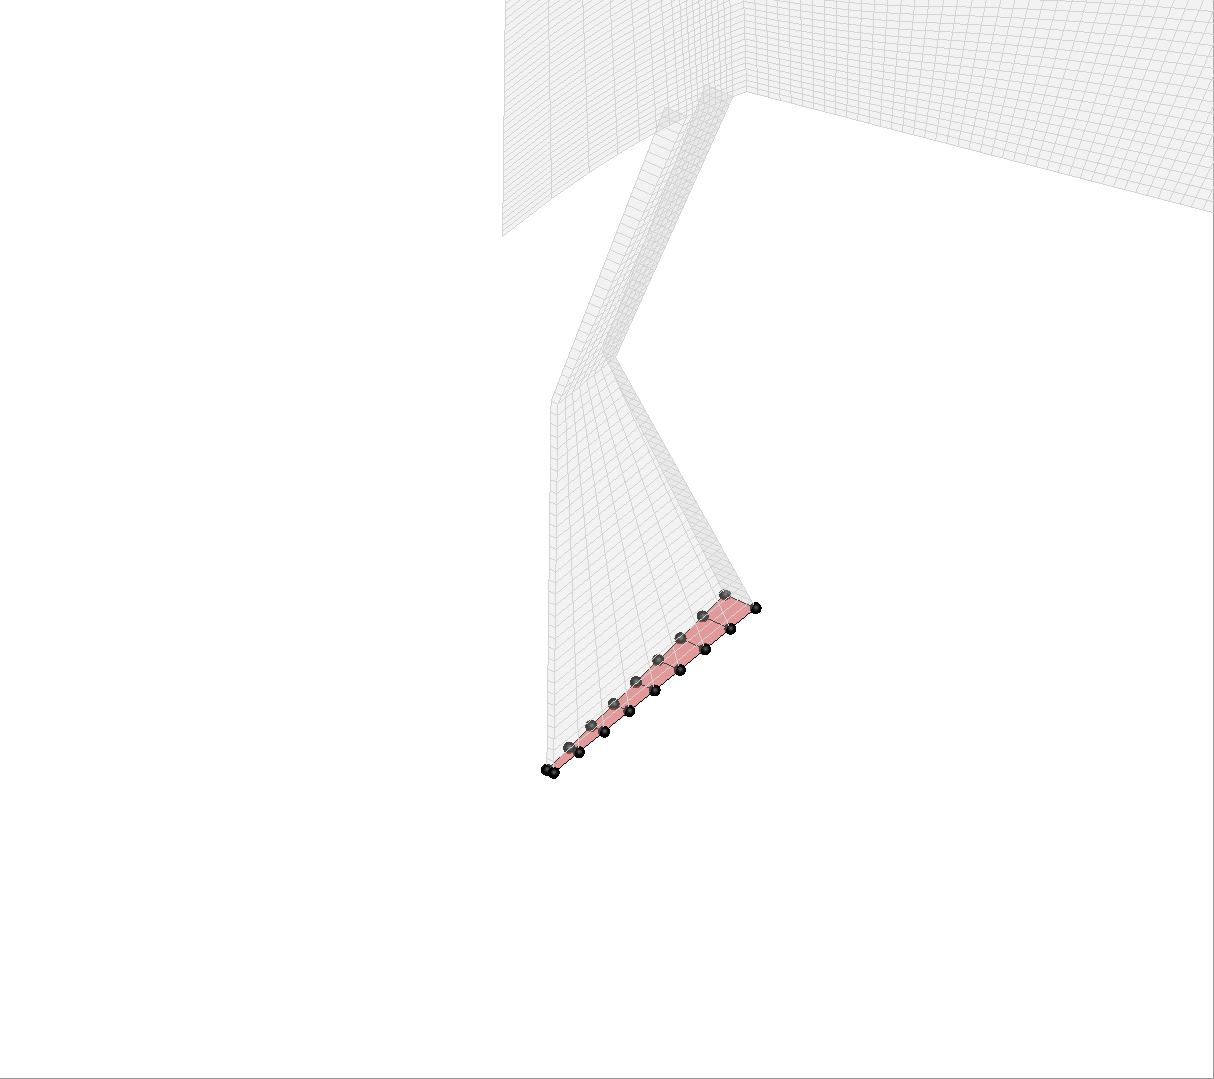
\includegraphics[width=\textwidth]{figures/plenum_bc.png}
    \caption{Mass Flow Rate Integrated Area}
    \label{fig:plenum-face}
  \end{subfigure}
\end{figure}
%------------------------------------------------------------------------------%

The mass flow rate, $\massflow$,
through the area outlined in \fref{fig:plenum-face} is computed as
%------------------------------------------------------------------------------%
\begin{equation}
  \massflow = \sum_{i}^{N_{faces}}\left( \rho_i \overline{U} A \right)
  \label{mass-flow-eqn}
\end{equation}
%------------------------------------------------------------------------------%
and is used a metric for the amount of propellent that is required to be carried
by the vehicle for blowing.  Again, for the purposes of this demonstration
problem, a lower mass flow rate at the plenum is equated to less total vehicle
mass.

\section{Composite Cost Function Definition and Components}
\label{cost-func-components}

The cost function (or objective function) as formulated in FUN3D is a composite,
weighted function
%------------------------------------------------------------------------------%
\begin{equation}
  f = \sum_{j=1}^{N_{func}}w_j\left( C_j - C_{j^*} \right)^{p_j}
  \label{generic-cost-function}
\end{equation}
%------------------------------------------------------------------------------%
Where $w_j$, $C_{j^*}$, and $p_j$ are the weight, target, and power of cost
function component $j$.  $C_j$ is the component value, which is evaluated at
each flow solution.  For example, an optimization problem that seeks to minimize the
surface temperature RMS without decreasing the drag, the cost function is
defined as 
%------------------------------------------------------------------------------%
\begin{equation}
  f = w_1\left( T_{RMS} \right)^{2} + w_2\left( C_{D} - C_{D}^{*} \right)^2
  \label{cd-tt-cost-function}
\end{equation}
%------------------------------------------------------------------------------%
For this case the component weights must be determined heuristically, to normalize
the changes in drag coefficient, $C_D$, and surface temperature Root-Mean-Square
(RMS) $T_{RMS}$.  The terms in \eref{cd-tt-cost-function} are squared to provide
a convex design space.

\section{Design Variables}

The design variables for the optimization problem are the plenum total pressure,
$P_{p,o}$, plenum total temperature, $T_{p,o}$, and plenum ``fuel-air ratio'',
$\fa$.  These are provided explicitly in the optimization problem, and are used
to directly set the flow conditions on plenum face boundary condition in the
nozzle, shown in \fref{fig:plenum-face}.  For a reacting gas mixture, the
``fuel-air ratio'' specifies the mass fractions for two species leaving the
plenum.  For example, if an $H_2-N_2$ mixture is ejected from the annular
nozzle, the mass fractions of $H_2$ and $N_2$ are given by
%------------------------------------------------------------------------------%
\begin{equation}
  \begin{aligned}
    c_{H_2} &= \fa \\
    c_{N_2} &= 1 - \fa
  \end{aligned}
  \label{fuel-air-def}
\end{equation}
%------------------------------------------------------------------------------%
Thus, the ratio $\fa$ dictates the mass fractions for two species injected into
the domain via the plenum boundary.

\section{Obtaining Sensitivity Gradients for Design Variables}

The sensitivity gradients for the plenum design variables are easily obtained by
manipulating \eref{obj-function} to obtain
%------------------------------------------------------------------------------%
\begin{equation}
  \pd{L}{\md} = \pd{f}{\md} + \rtdiff{}{\md} \mathbf{\Lambda}
  \label{obj-linearization1}
\end{equation}
%------------------------------------------------------------------------------%
For the cost function components listed in \sref{cost-func-components}, there is
no direct dependence on the plenum design variables; thus,
\eref{obj-linearization1} can be reduced to
%------------------------------------------------------------------------------%
\begin{equation}
  \pd{L}{\md} = \rtdiff{}{\md} \mathbf{\Lambda}
  \label{obj-linearization2}
\end{equation}
%------------------------------------------------------------------------------%
Once the adjoint co-state variables $\mathbf{\Lambda}$ have been computed by
solving the adjoint equations (\eref{adjoint-main}) the sensitivity derivatives
of the cost function with respect to the plenum design variables are obtained by
evaluating relatively inexpensive matrix-vector products.

\section{Inverse Design Optimization}
\label{inv-design-opt}

The optimization procedure is done using the \textit{opt\_driver} utility in
FUN3D, which is a wrapper utility that executes the FUN3D flow solver, adjoint
solver, and optimization algorithm sequentially.  These steps are repeated until
a termination criterion is reached.  In practice, the termination of the
optimization occurs when the cost function reaches a tolerance of less that
$10^{-8}$, or when continuing towards the optimal condition would exceed the
prescribed upper or lower bounds of the design variables.

%------------------------------------------------------------------------------%
\begin{figure}[h]
  \centering
	\begin{subfigure}[b]{0.45\textwidth}
    \centering
    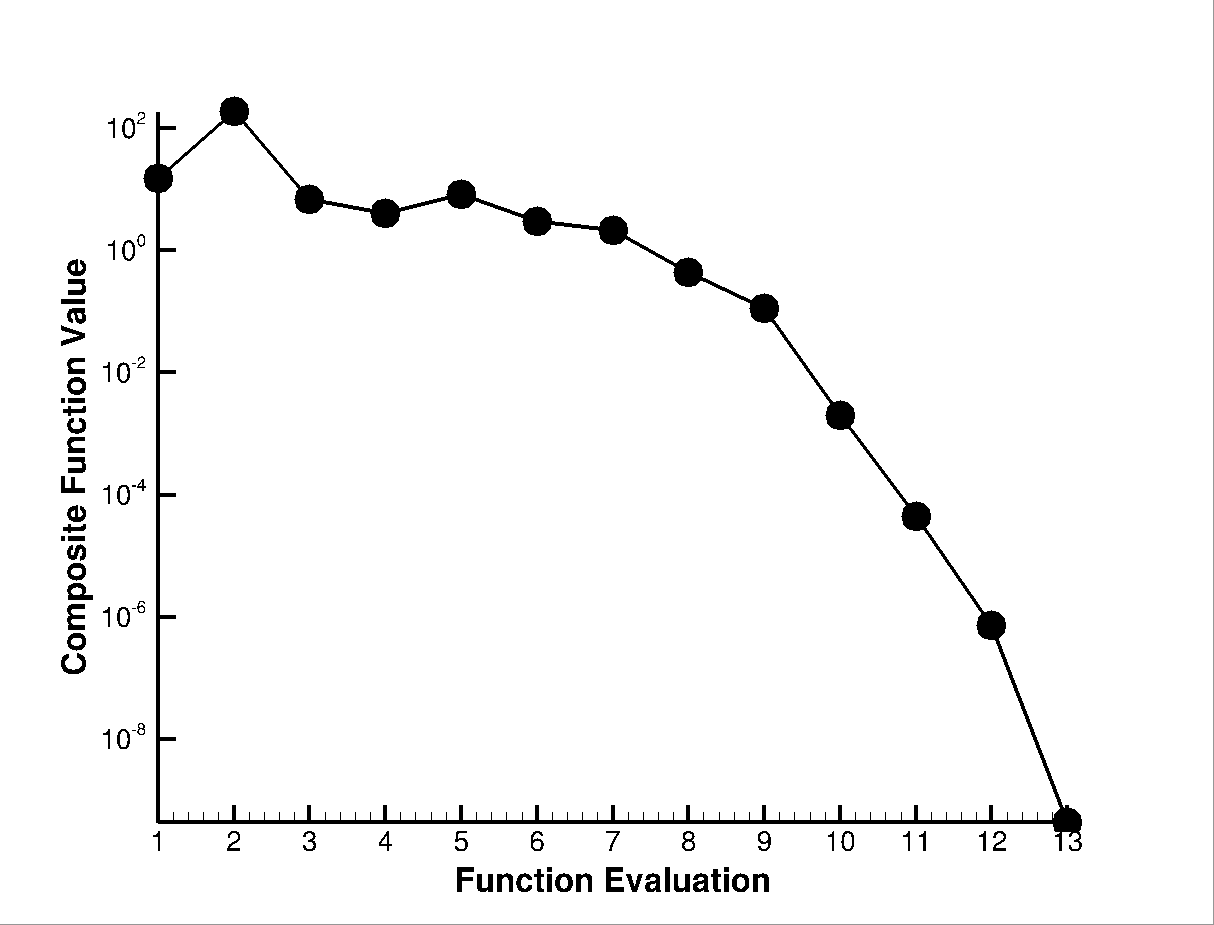
\includegraphics[width=\textwidth]{figures/1st-H2/cost_func.png}
    \caption{Composite Value}
    \label{fig:cost-func-1st-H2}
  \end{subfigure}
	\begin{subfigure}[b]{0.45\textwidth}
    \centering
    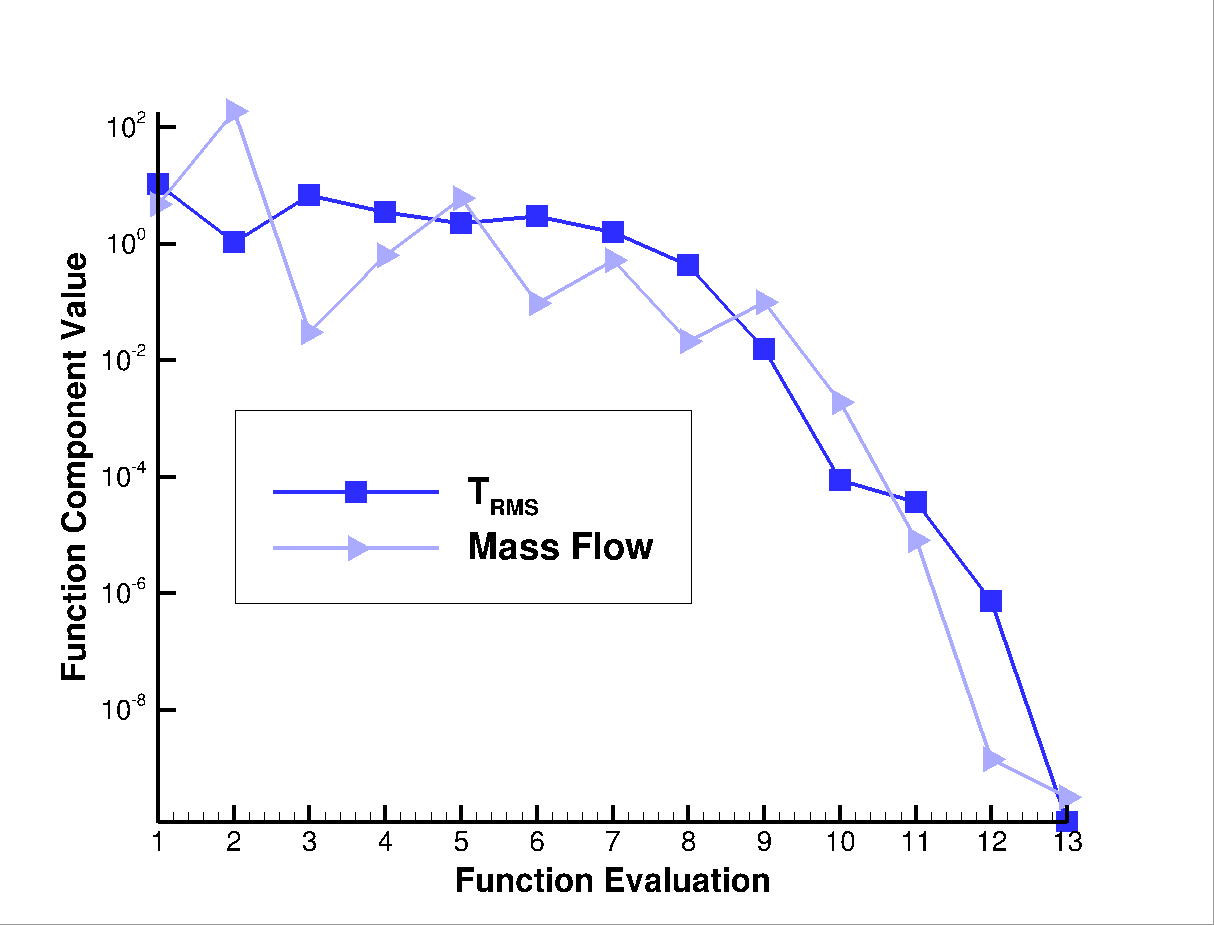
\includegraphics[width=\textwidth]{figures/1st-H2/func_components.png}
    \caption{Component Values}
    \label{fig:components-1st-H2}
  \end{subfigure}
  \caption{Cost Function and Component History}
\end{figure}
%------------------------------------------------------------------------------%
To demonstrate the inverse design capability of an adjoint-based design
optimization, targets of 2000 K for the surface temperature RMS and 0.0024
$kg/s$ for the annular nozzle mass flow rate were specified.  These targets were
chosen semi-arbitarily, and were heuristically determined to be feasible based
the the design variable bounds. The design variables specified for this
optimization were the plenum total pressure, $P_{p,o}$ and the plenum ``fuel-air
ratio'', $\fa$.  A species mixture consisting of $H_2$ and $N_2$ was blown from
the plenum, with the mass fractions dictated by $\fa$ as described in
\eref{fuel-air-def}.  For the cost function, the weights were chosen
heuristically, such that 
%------------------------------------------------------------------------------%
\begin{equation}
  \frac{w_1}{w_2} = \frac{\cost{T_{RMS}}^2}{\cost{\dot{m}}^2}
  \label{weight-ratio}
\end{equation}
%------------------------------------------------------------------------------%
This results in a roughly equivalent weighting beween the $T_{RMS}$ and
$\dot{m}$, which is desired as both targets should be met at optimality.
%------------------------------------------------------------------------------%
\begin{figure}[h]
  \centering
  \begin{subfigure}[b]{0.45\textwidth}
    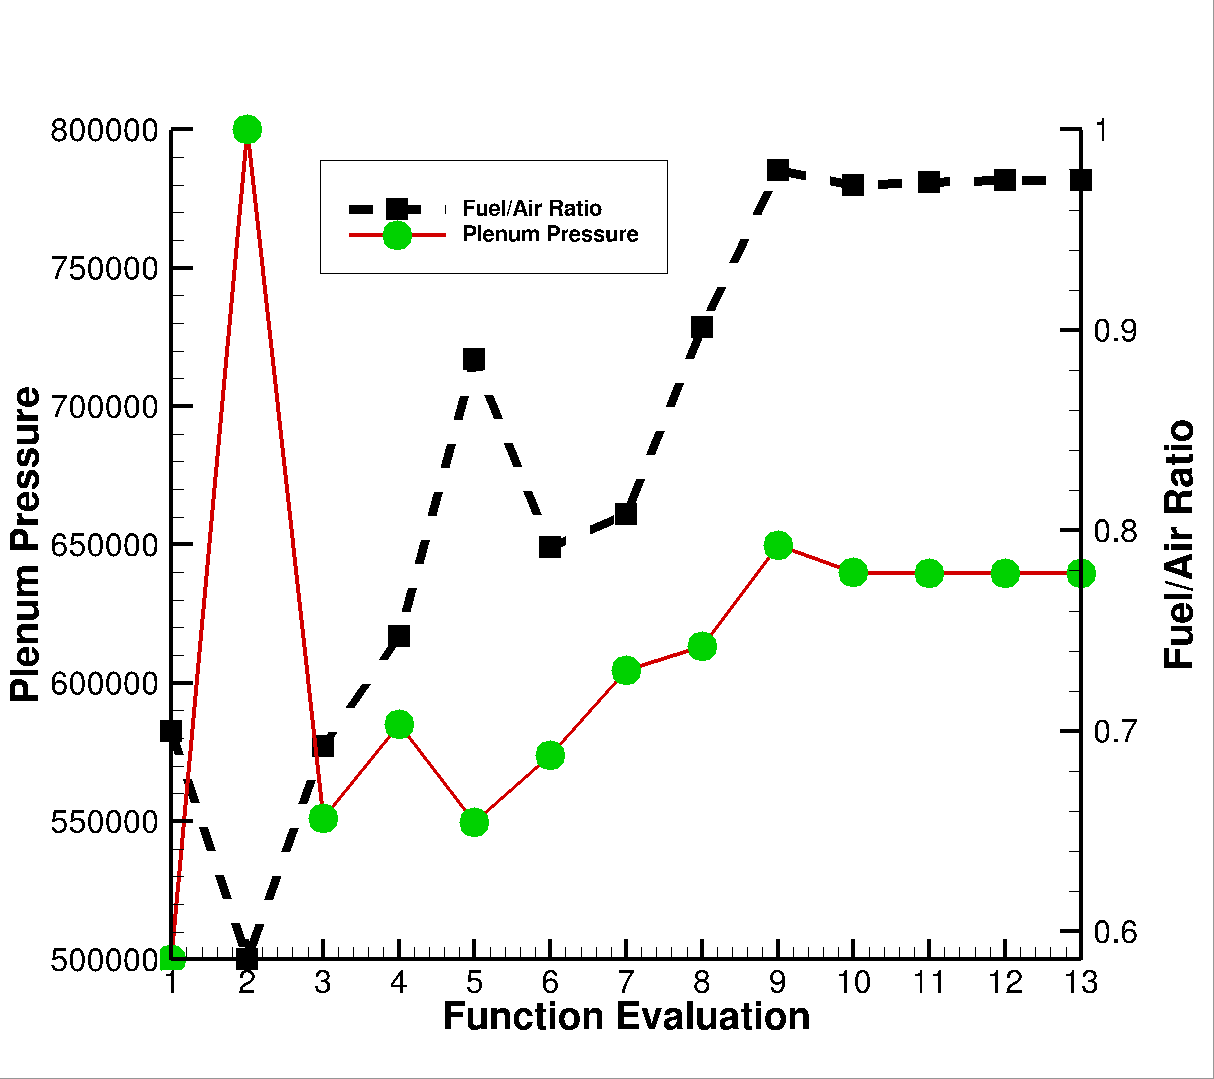
\includegraphics[width=\textwidth]{figures/1st-H2/dv_hist.png}
    \caption{Design Variable History}
    \label{fig:dv-hist-1st-H2}
  \end{subfigure}
  \begin{subfigure}[b]{0.45\textwidth}
    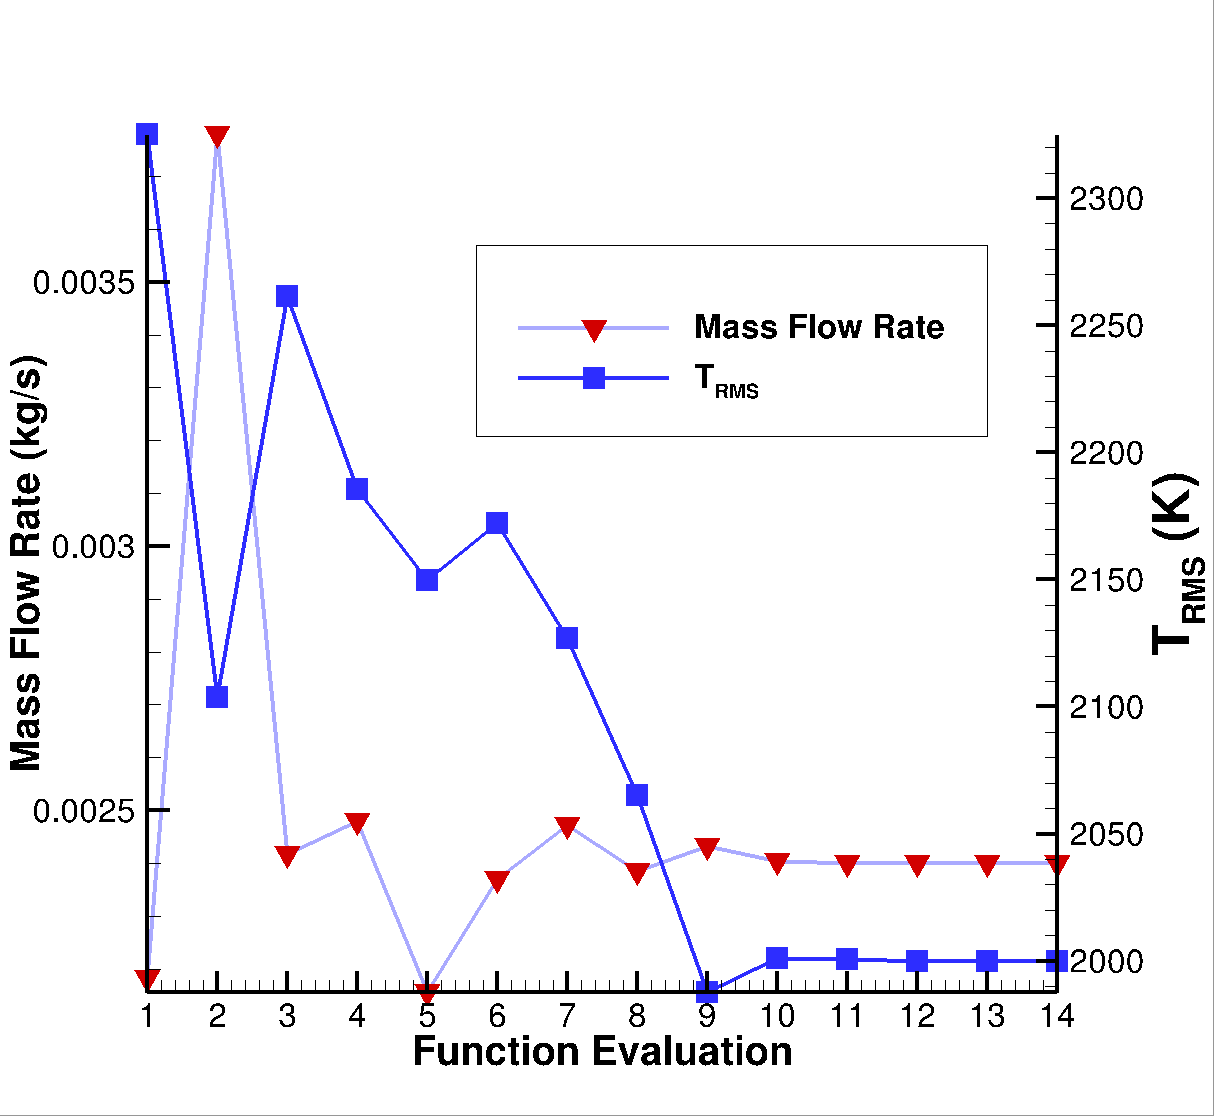
\includegraphics[width=\textwidth]{figures/1st-H2/fm_hist.png}
    \caption{Design Variable History}
    \label{fig:fm-hist-1st-H2}
  \end{subfigure}
  \caption{Inverse Design History}
\end{figure}
%------------------------------------------------------------------------------%
Using the SNOPT optimizer, \fref{fig:cost-func-1st-H2} shows that the target
design was met within 13 function evaluations.  SNOPT explores the entire design
space, as is show in the second function evaluation, where a spike in the cost
function occurred.
\fref{fig:dv-hist-1st-H2} indicates that the optimizer tried the upper
bound for the plenum pressure design variable, and found that sensitivity
derivatives indicated that the lower pressure was required. This is common, and
is an effective way to insure that there is a local minimum in the prescribed
bound.  The optimization terminated when the cost function value was less than
the tolerance of $10^{-8}$, and \fref{fig:components-1st-H2} shows that both
components of the cost function were within one order of magnitude of each other
during the optimization.  This last point is important, since non-normalized
components can skew the optimization results, where competing components can
cause oscillations in the function evaluations and stall the optimization
procedure.  \fref{fig:fm-hist-1st-H2} shows the history of the surface
temperature RMS and annular nozzle mass flow rate, with the design targets.  The
optimization clearly made significant progress early, with smaller gains as the
solution approached the target.

\section{Direct Design Optimization}

Using the same cost function components and design variables as in
\sref{inv-design-opt}, a direct design problem was completed to minimize both
mass flow rate and surface temperature RMS.  The cost function was formulated as
%------------------------------------------------------------------------------%
\begin{equation}
  f = w_1\left( \massflow \right)^2 + w_2\left( T_{RMS} \right)^2
  \label{direct-design-cost-func}
\end{equation}
%------------------------------------------------------------------------------%
With the weights chosen in the same manner as the inverse design problem to
insure that the components are normalized to the same order of magnitude
%------------------------------------------------------------------------------%
\begin{equation}
  \frac{w_1}{w_2} = \frac{\left( \massflow \right)^2}{\left( T_{RMS} \right)^2}
  \label{direct-design-weights}
\end{equation}
%------------------------------------------------------------------------------%
The SNOPT optimizer was able to very quickly determine that blowing pure
$H_2$, i.e. $\fa = 1.0$, would yield the lowest surface temperature RMS and mass
flow rate.  \fref{fig:dd-cost-func-value} shows that most of the improvement in
the design was made within the first two function evaluations, and the
subsequent steps were significantly less.
%------------------------------------------------------------------------------%
\begin{figure}[h]
  \centering
	\begin{subfigure}[b]{0.4\textwidth}
    \centering
    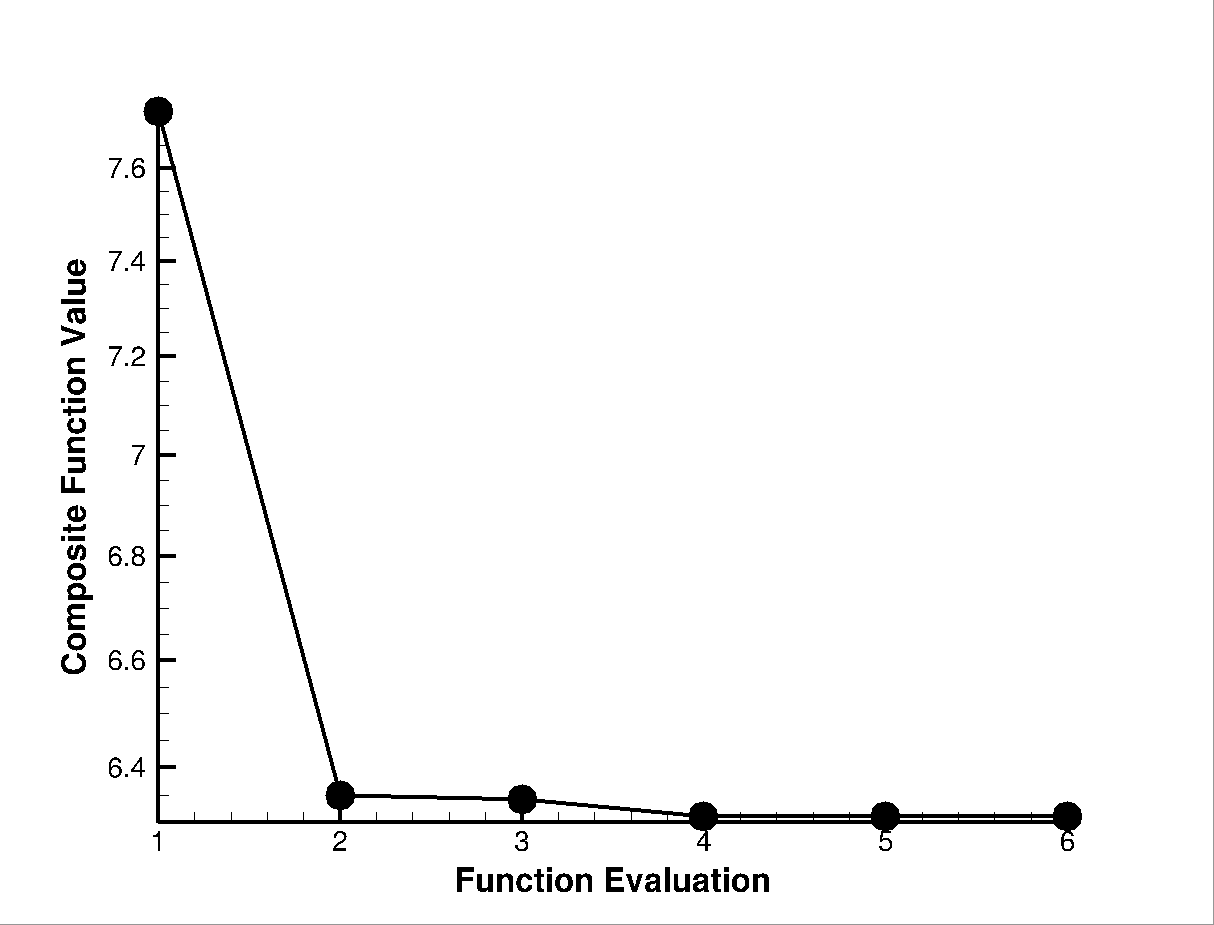
\includegraphics[width=\textwidth]{figures/direct_design/cost-func.png}
    \caption{Composite Cost Function Value}
    \label{fig:dd-cost-func-value}
  \end{subfigure}
	\begin{subfigure}[b]{0.4\textwidth}
    \centering
    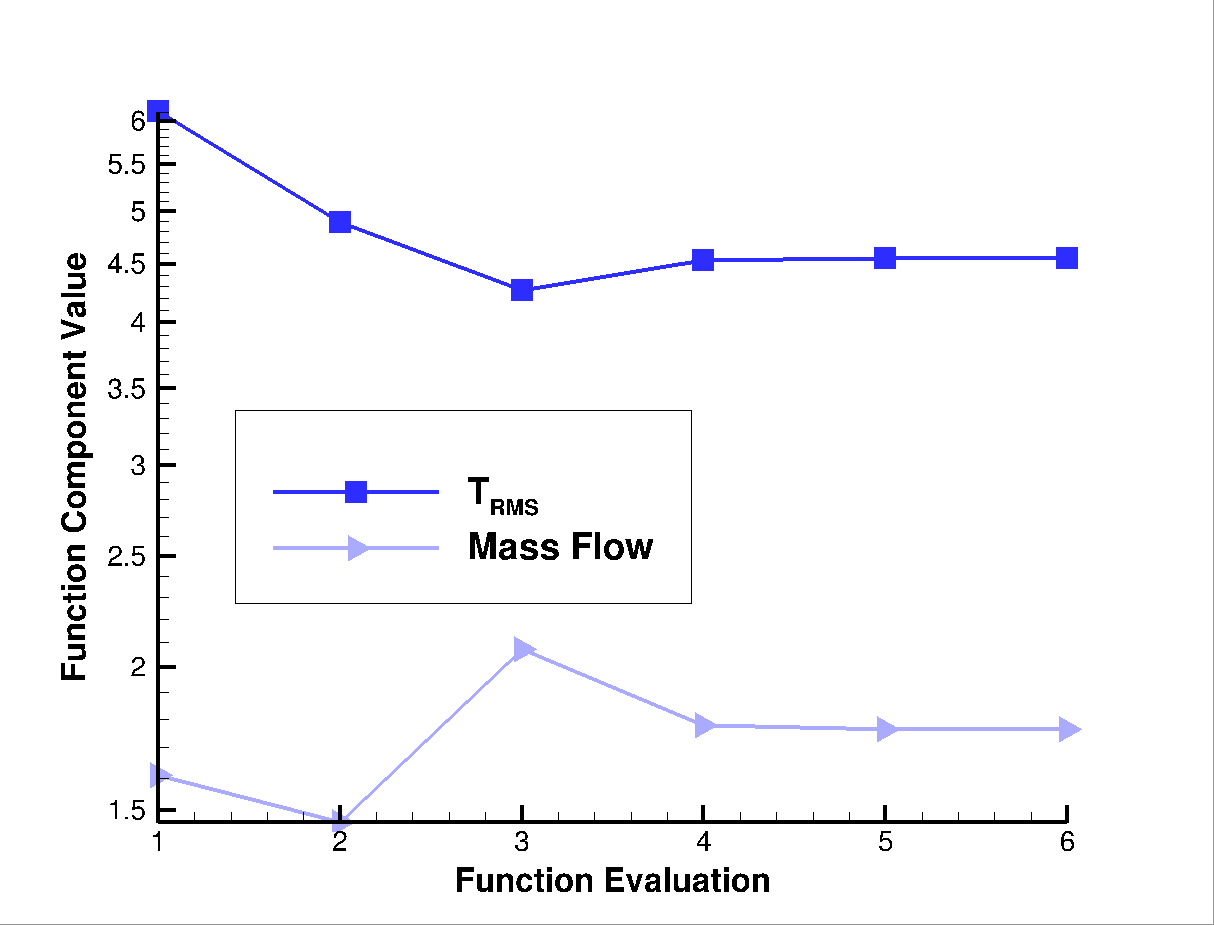
\includegraphics[width=\textwidth]{figures/direct_design/components.png}
    \caption{Cost Function Components}
    \label{fig:dd-components}
  \end{subfigure}
  \caption{Direct Design Cost Function}
  \label{fig:dd-cost-func}
\end{figure}
%------------------------------------------------------------------------------%
\fref{fig:dd-components} verifies that weights determined by
\eref{direct-design-weights} were indeed sufficient to normalize $\massflow$ and
$T_{RMS}$ contributions to the composite cost function.
%------------------------------------------------------------------------------%
\begin{figure}[h]
  \centering
	\begin{subfigure}[b]{0.4\textwidth}
    \centering
    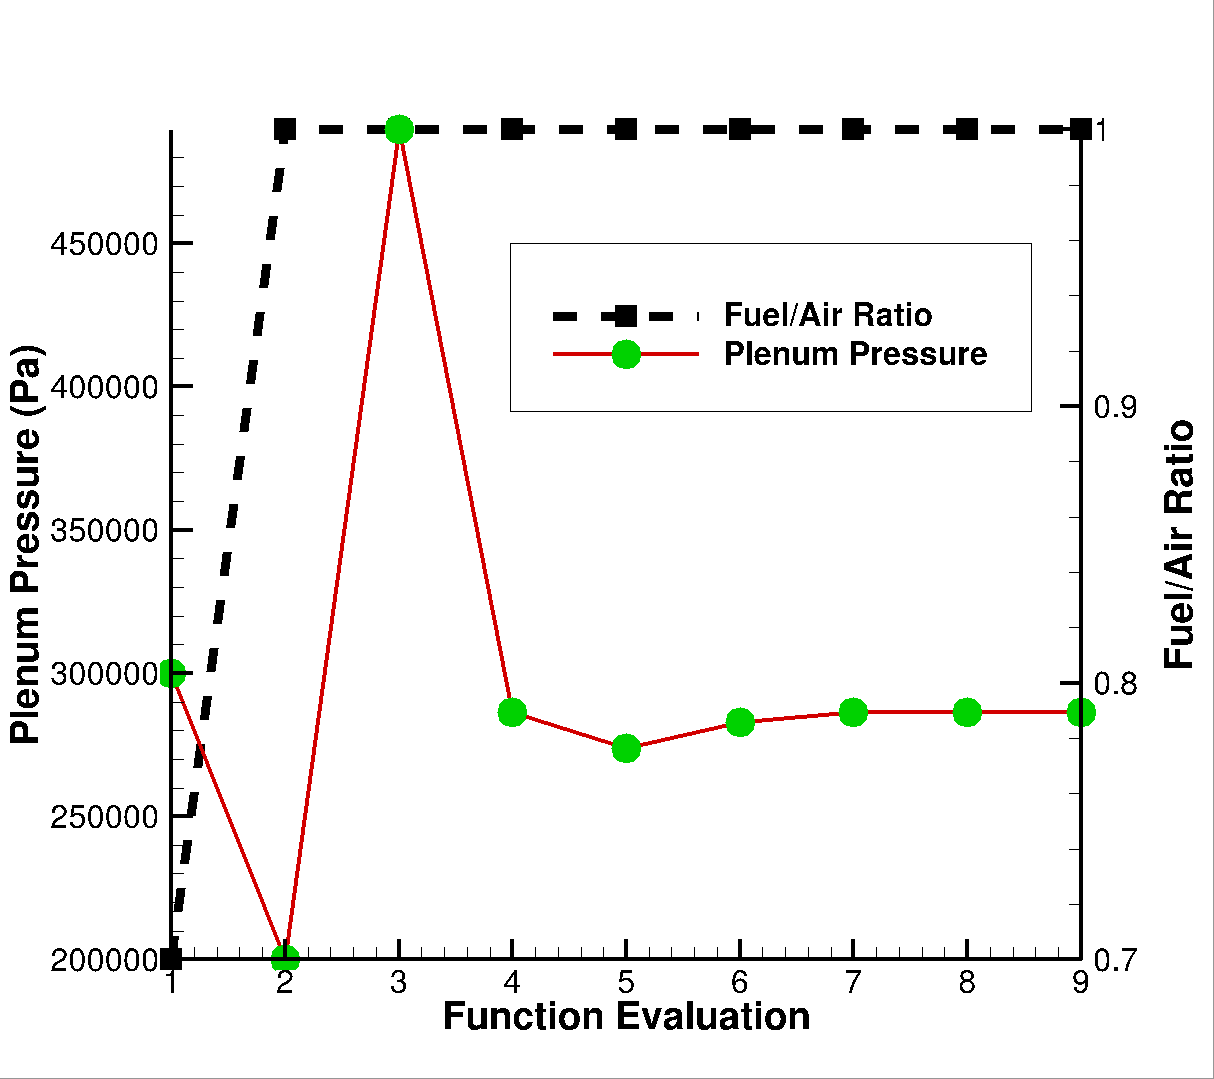
\includegraphics[width=\textwidth]{figures/direct_design/dv-hist.png}
    \caption{Design Variable History}
    \label{fig:dd-dv-hist}
  \end{subfigure}
	\begin{subfigure}[b]{0.4\textwidth}
    \centering
    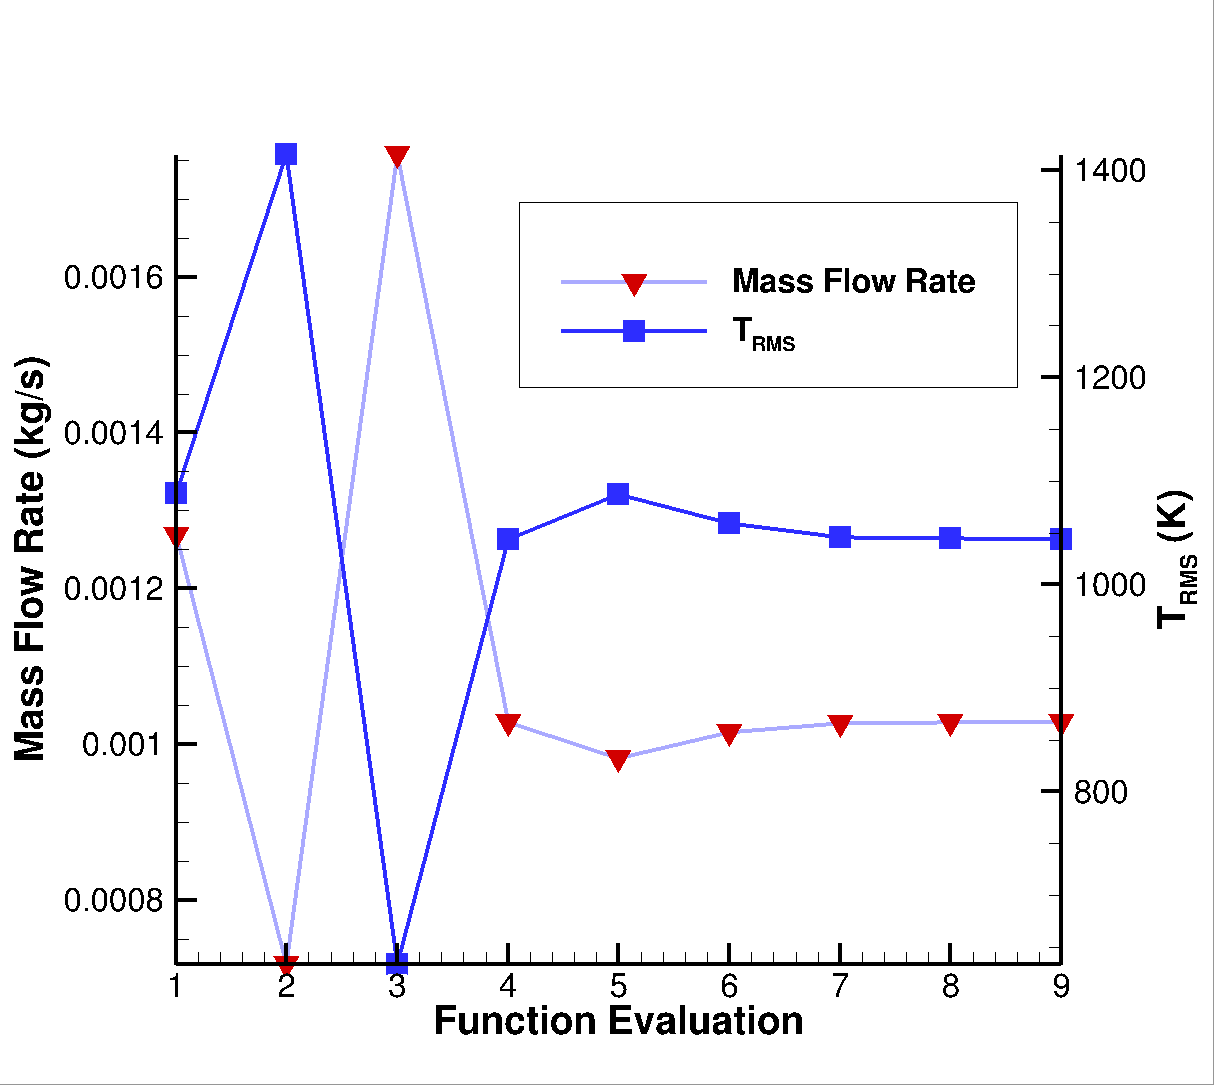
\includegraphics[width=\textwidth]{figures/direct_design/mass-tt.png}
    \caption{$\massflow$ and $T_{RMS}$ Design History}
    \label{fig:dd-mass-tt}
  \end{subfigure}
  \caption{Direct Design History}
  \label{fig:dd-history}
\end{figure}
%------------------------------------------------------------------------------%
\fref{fig:dd-dv-hist} shows that the optimization was largely dependent on the
plenum pressure, and \tref{tab:design-improvement} shows that larger pressure at
the plenum resulted in a 13.79\% lower surface temperature, at the expense of a
4.6\% higher mass flow rate.
%------------------------------------------------------------------------------%
\begin{table}[h]
  \centering
  \begin{tabular}{c|c|c|c}
    Component & Initial & Final & Improvement\\
    \hline
    $\dot{m}$, $kg/s$ & 1.268e-3 & 1.327e-3 & -4.6\% \\
    $T_{RMS}$, $K$    & 2473     & 2132     & 13.79\%
  \end{tabular}
  \caption{Direct Design Optimization Improvement}
  \label{tab:design-improvement}
\end{table}
%------------------------------------------------------------------------------%
This is an excellent problem for a high-fidelity gradient-based
optimization, as the non-linear effects of plenum-shock interation makes the
optimum plenum condition difficult to determine intuitively.

There is a much stronger dependence on the choice of cost function weights for
this problem than for the inverse design problem in \sref{inv-design-opt}.  For
the inverse design problem, the target mass flow rate and surface temperature
RMS were known a priori; therefore, the weighting was chosen as a purely
normalizing measure to accelerate convergence to the target condition.  For this
direct design problem the target mass flow rate and surface temperature RMS are
not know a priori, and the weights chosen have a direct impact on the optimum
condition.  A ``skewed'' weighting may be advisable from an engineering
perspective when attempting a direct design approach.  For example, if the
surface thermal protection (TPS) is rated to withstand much higher surface
heating than what is nominally predicted, a higher weight might be given to the
mass flow rate in order to decreased the required vehicle mass.  The heuristic
nature of this approach can be avoided by setting a component target, or
converting a composite cost function component to an explicit constraint.  The
latter option is more robust, but comes at the cost of an additional adjoint
solution.



%%---------------------------------------------------------------------------%%
%%  Bibliography 

\bibliography{KyleThompson-thesis}{}
\bibliographystyle{plain}

%%---------------------------------------------------------------------------%%
% Appendices
\appendix

\chapter{Derivations}
\label{derivations}

\section{Decoupled Flux Derivation}
\label{decoupled-flux-derivation}

For the Roe flux difference splitting scheme, the species mass fluxes are given by
%------------------------------------------------------------------------------%
\begin{equation}
	F_{\rho_s} = \frac{\rho_s^L\overline{U}^L+\rho_s^R\overline{U}^R}{2}
	-\frac{\tilde{c}_s(\lambda_1 dv_1 + \lambda_2 dv_2)+\lambda_3 dv_{3_s}}{2}
  \label{species-mass} \\
\end{equation}
\begin{align}	
		dv_1 &= \frac{p^R-p^L+\tilde{\rho} \tilde{a} (\overline{U}^R-\overline{U}^L)}{\tilde{a}^2} \\
		dv_2 &= \frac{p^R-p^L-\tilde{\rho} \tilde{a} (\overline{U}^R-\overline{U}^L)}{\tilde{a}^2} \\
		dv_{3_s} &= \frac{\tilde{a}^2 (\rho_s^R-\rho_s^L)- \tilde{c}_s (p^R-p^L)}{\tilde{a}^2}
\end{align}
\begin{align}
	\lambda_1 = \mid\mathbf{\overline{U}}+\tilde{a} \mid,\quad 
	\lambda_2 = \mid \mathbf{\overline{U}}-\tilde{a} \mid,\quad 
	\lambda_3 =  \mid \mathbf{\overline{U}} \mid
\end{align}
%------------------------------------------------------------------------------%
where the $\tilde{}$ notation signifies a Roe-averaged quantity, given by:
%------------------------------------------------------------------------------%
\begin{gather}
	\mathbf{\tilde{U}} =\roe \mathbf{\tilde{U}}^L+(1-\roe)\mathbf{\tilde{U}}^R \\
	\roe = \frac{\tilde{\rho}}{\tilde{\rho}+\rho^R} \\
	\tilde{\rho} = \sqrt{\rho^R\rho^L}
\end{gather}
%------------------------------------------------------------------------------%
The species mass fluxes must sum to the total mass flux; thus, the total mixture
mass flux is given as
%------------------------------------------------------------------------------%
\begin{equation}
\label{total-mass}
	F_\rho = \sum\limits_{s}{F_{\rho_s}} = \frac{\rho^L\overline{U}^L+\rho^R\overline{U}^R}{2}
	-\frac{\lambda_1 dv_1 + \lambda_2 dv_2 +\lambda_3 dv_3}{2}
\end{equation}
\begin{equation}
	dv_3 = \frac{\tilde{a}^2 (\rho^R-\rho^L)-(p^R-p^L)}{\tilde{a}^2}
\end{equation}
%------------------------------------------------------------------------------%
Multiplying \eref{total-mass} by the Roe-averaged mass fraction and
substituting it into \eref{species-mass} results in:
%------------------------------------------------------------------------------%
\begin{equation}
\label{unsimp-sp-flux}
	F_{\rho_s} =\tilde{c}_s F_\rho + \frac{(c_s^L-\tilde{c}_s)\rho^L(\overline{U}^L+\mid \tilde{U}\mid)}{2}
	+ \frac{(c_s^R-\tilde{c}_s)\rho^R(\overline{U}^R-\mid \tilde{U}\mid)}{2}
\end{equation}
%------------------------------------------------------------------------------%
It should be noted here that the Roe-averaged normal velocity, $\tilde{U}$,
requires an entropy correction in the presence of strong shocks\cite{harten}.
This correction has a dependence on the roe-averaged speed of sound, and
therefore has a dependence on the species mass fractions; however,
through numerical experiments it has been determined that omitting this
dependence does not adversely affect convergence.  The notation can be further
simplified by defining the normal velocities as follows:
%------------------------------------------------------------------------------%
\begin{equation}
  \lambda^+ = \frac{\overline{U}^L+\mid \tilde{U}\mid}{2}, \quad 
  \lambda^- = \frac{\overline{U}^R-\mid \tilde{U}\mid}{2} 
  \label{lambda-pm} 
\end{equation}
%------------------------------------------------------------------------------%
Finally, substituting \eref{lambda-pm} into \eref{unsimp-sp-flux} yields the
final result for calculating the species flux in the decoupled system:
%------------------------------------------------------------------------------%
\begin{equation}
  F_{\rho_s} =
  \tilde{c}_s F_\rho 
  + (c_s^L-\tilde{c}_s)\rho^L\lambda^+ 
  + (c_s^R-\tilde{c}_s)\rho^R\lambda^-
  \label{sp-flux} 
\end{equation}
%------------------------------------------------------------------------------%
Forming the convective contributions to the Jacobians is straightforward.
Because the $\mathbf{U}'$ level variables are constant, only the left, right,
and Roe-averaged state mass fractions vary.  Differentiating \eref{sp-flux}
with respect to the mass fraction, $c_s$, the left and right state contributions
are
%------------------------------------------------------------------------------%
\begin{gather}
  \pd{F_{\rho_s}}{c^L_s} = \roe F_\rho+(1-\roe)\rho^L\lambda^+ - \roe \rho^R\lambda^- \\
  \pd{F_{\rho_s}}{c^R_s} = (1-\roe) F_\rho+(\roe-1)\rho^L\lambda^+ + \roe\rho^R\lambda^- 
  \label{dc-sp-linearizations}
\end{gather}
%------------------------------------------------------------------------------%
Because there is no dependence between species in decoupled convective
formulation, the Jacobian block elements are purely diagonal for the convective
contributions, of the form
%------------------------------------------------------------------------------%
\begin{equation} 
  \begin{pmatrix} 
    \pd{F_{\rho_1}}{c_1} & & 0 \\ 
    & \ddots & \\ 
    0 & & \pd{F_{\rho_{ns}}}{c_{ns}}
  \end{pmatrix}
  \label{dc-diag-Jacobian}
\end{equation}
%------------------------------------------------------------------------------%

\section{Quadratic Interpolation Between Thermodynamic Curve Fits}
\label{sec:quad-cp-blending}

We seek to blend the two thermodynamic curve fits in such a way that we maintain
$c_0$ continuity in both specific heat ($C_p$) and enthalpy ($h$).  To
accomplish this, a quadratic function must be used, of the form
%------------------------------------------------------------------------------%
\begin{equation}
  a T^2 + b T + c = C_p
  \label{generic_form}
\end{equation}
%------------------------------------------------------------------------------%
The coefficients $a$, $b$, and $c$ are determined by solving the system that
results from the boundary value problem
%------------------------------------------------------------------------------%
\begin{equation}
  \begin{cases}
    a {T_1}^{2} + b T_1 +c = C_{p_1} \\
    a {T_2}^{2} + b T_2 +c = C_{p_2} \\
    a \frac{\left( {T_2}^{3} - {T_1}^{3}\right) }{3} + b\frac{ \left( {T_2}^{2} - {T_1}^{2}\right) }{2} + c \left( T_2 - T_1\right) = h_2-h_1
  \end{cases}
\end{equation}
%------------------------------------------------------------------------------%
Where the $x_1$ and $x_2$ subscripts describe the left and right states,
respectively.  Solving the linear system, the coefficients are
%------------------------------------------------------------------------------%
\begin{equation}
  \begin{cases}
    a=\frac{3\left( C_{p_2}+ C_{p_1}\right) }{(T_2-T_1)^{2}} - \frac{6 \left(h_2 - h_1\right)}{(T_2-T_1)^{3}}\\ \\
    b=-\frac{2\left[(C_{p_2} + 2C_{p_1})T_2 + (2C_{p_2} + C_{p_1})T_1\right]}{(T_2-T_1)^{2}} + \frac{6(T_2+T_1)(h_2 - h_1)}{(T_2 - T_1)^3}\\ \\
    c=\frac{C_{p_1} T_2 (T_2 + 2T_1) + C_{p_2} T_1 (T_1 + 2 T_2)}{(T_2-T_1)^2} - \frac{6 T_1 T_2 (h_2 - h_1)}{(T_2 - T_1)^3}
  \end{cases}
\end{equation}
%------------------------------------------------------------------------------%
This can be simplified to
%------------------------------------------------------------------------------%
\begin{gather}
  \begin{cases}
    a=3B - A \\ \\
    b=\frac{-2(C_{p_1} T_2 + C_{p_2}T_2)}{(T_2 - T_1)^2} +(T_2+T_1) (A - 2B) \\ \\
    c=\frac{C_{p_1} {T_2}^2 + C_{p_2} {T_1}^2}{(T_2-T_1)^2} + T_1 T_2 (2B - A)
  \end{cases} \\
  A = \frac{6(h_2 - h_1)}{(T_2 - T_1)^3} \\
  B = \frac{C_{p_2} + C_{p_1}}{(T_2 - T_1)^2}
\end{gather}
%------------------------------------------------------------------------------%
Note that this does not ensure that entropy will be continuous across curve
fits.

\section{Change of Variable Sets}
\label{change-of-var-section}

The decoupled scheme developed by Candler et. al\cite{candler} is based upon the
change of variables
%------------------------------------------------------------------------------%
\begin{equation}
  \mU = \begin{pmatrix}
    \rho_1 \\
    \vdots \\
    \rho_{ns} \\
    \rho \vu \\
    \rho E
  \end{pmatrix}
  \rightarrow
  \mv = \begin{pmatrix}
    c_1 \\
    \vdots \\
    c_{ns} \\
    \rho \\
    \rho \vu \\
    \rho E
  \end{pmatrix}
  \label{var-sets}
\end{equation}
%------------------------------------------------------------------------------%
To avoid confusion between variable sets, we re-write the variable vectors,
$\mU$ and $\mv$, in a more generic sense
%------------------------------------------------------------------------------%
\begin{equation}
  \mU = \begin{pmatrix}
    u_1 \\
    \vdots \\
    u_{ns + 2}
  \end{pmatrix}
  \rightarrow
  \mv = \begin{pmatrix}
    v_1 \\
    \vdots \\
    v_{ns + 3}
  \end{pmatrix}
  \label{generic-var-sets}
\end{equation}
%------------------------------------------------------------------------------%
For simplicity, consider a system with two species, $\rho_1$ and $\rho_2$.
Using the relationship $\rho_s = c_s \rho$, then the original variable vector,
$\mU$ can be rewritten in terms of the new variables, $\mv$ as
%------------------------------------------------------------------------------%
\begin{equation}
  \mU = \begin{pmatrix}
    u_1 \\
    u_2 \\
    u_3 \\
    u_4
  \end{pmatrix}
  =
  \begin{pmatrix}
    v_1 v_3 \\
    v_2 v_3 \\
    v_4 \\
    v_5
  \end{pmatrix}
  \label{u-to-v}
\end{equation}
%------------------------------------------------------------------------------%
This allows the derivation of the Jacobian 
%------------------------------------------------------------------------------%
\begin{equation}
  \pd{\mU}{\mv} = 
  \begin{pmatrix}
    \pd{u_1}{v_1} & \pd{u_1}{v_2} & \pd{u_1}{v_3} & \pd{u_1}{v_4} & \pd{u_1}{v_5} \\ \\
    \pd{u_2}{v_1} & \pd{u_2}{v_2} & \pd{u_2}{v_3} & \pd{u_2}{v_4} & \pd{u_2}{v_5} \\ \\
    \pd{u_3}{v_1} & \pd{u_3}{v_2} & \pd{u_3}{v_3} & \pd{u_3}{v_4} & \pd{u_3}{v_5} \\ \\
    \pd{u_4}{v_1} & \pd{u_4}{v_2} & \pd{u_4}{v_3} & \pd{u_4}{v_4} & \pd{u_4}{v_5}
  \end{pmatrix}
  =
  \begin{pmatrix}
    v_3 & 0   & v_1 & 0 & 0 \\ \\
    0   & v_3 & v_2 & 0 & 0 \\ \\
    0   & 0   & 0   & 1 & 0 \\ \\
    0   & 0   & 0   & 0 & 1
  \end{pmatrix}
  \label{dudv-jac}
\end{equation}
%------------------------------------------------------------------------------%
At this point, it is important to note that the Jacobian in \eref{dudv-jac} has
two psuedo-inverse matricies, that correspond to the right and left inverse.
The right inverse, $\pdr{\mv}{\mU}{R}$, can be constructed based on the previously
defined steps
%------------------------------------------------------------------------------%
\begin{equation}
  \pdr{\mv}{\mU}{R} = 
  \begin{pmatrix}
    \pd{v_1}{u_1} & \pd{v_1}{u_2} & \pd{v_1}{u_3} & \pd{v_1}{u_4} \\ \\
    \pd{v_2}{u_1} & \pd{v_2}{u_2} & \pd{v_2}{u_3} & \pd{v_2}{u_4} \\ \\
    \pd{v_3}{u_1} & \pd{v_3}{u_2} & \pd{v_3}{u_3} & \pd{v_3}{u_4} \\ \\
    \pd{v_4}{u_1} & \pd{v_4}{u_2} & \pd{v_4}{u_3} & \pd{v_4}{u_4} \\ \\
    \pd{v_5}{u_1} & \pd{v_5}{u_2} & \pd{v_5}{u_3} & \pd{v_5}{u_4} 
  \end{pmatrix}
  =
  \begin{pmatrix}
    \frac{1-v_1}{v_3} & \frac{-v_1}{v_3}  & 0 & 0 \\ \\
    \frac{-v_2}{v_3}  & \frac{1-v_2}{v_3} & 0 & 0 \\ \\
    1                 & 1                 & 0 & 0 \\ \\
    0                 & 0                 & 1 & 0 \\ \\
    0                 & 0                 & 0 & 1
  \end{pmatrix}
  \label{dvdu-jac-right}
\end{equation}
%------------------------------------------------------------------------------%
It is easily verified that the matrix product of
\erefs{dudv-jac}{dvdu-jac-right} produces identity
%------------------------------------------------------------------------------%
\begin{equation}
  \pd{\mU}{\mv} \pdr{\mv}{\mU}{R} = 
  \begin{pmatrix}
    v_3 & 0   & v_1 & 0 & 0 \\ \\
    0   & v_3 & v_2 & 0 & 0 \\ \\
    0   & 0   & 0   & 1 & 0 \\ \\
    0   & 0   & 0   & 0 & 1
  \end{pmatrix}
  \begin{pmatrix}
    \frac{1-v_1}{v_3} & \frac{-v_1}{v_3}  & 0 & 0 \\ \\
    \frac{-v_2}{v_3}  & \frac{1-v_2}{v_3} & 0 & 0 \\ \\
    1                 & 1                 & 0 & 0 \\ \\
    0                 & 0                 & 1 & 0 \\ \\
    0                 & 0                 & 0 & 1
  \end{pmatrix}
  =
  \begin{pmatrix}
    1 & 0 & 0 & 0 \\ \\
    0 & 1 & 0 & 0 \\ \\
    0 & 0 & 1 & 0 \\ \\
    0 & 0 & 0 & 1
  \end{pmatrix}
  \label{dvdu-jac-right-I}
\end{equation}
%------------------------------------------------------------------------------%
however, \eref{dvdu-jac-right-I} is not associative
%------------------------------------------------------------------------------%
\begin{equation}
  \begin{aligned}
    \pdr{\mv}{\mU}{R} \pd{\mU}{\mv} &= 
    \begin{pmatrix}
      \frac{1-v_1}{v_3} & \frac{-v_1}{v_3}  & 0 & 0 \\ \\
      \frac{-v_2}{v_3}  & \frac{1-v_2}{v_3} & 0 & 0 \\ \\
      1                 & 1                 & 0 & 0 \\ \\
      0                 & 0                 & 1 & 0 \\ \\
      0                 & 0                 & 0 & 1
    \end{pmatrix}
    \begin{pmatrix}
      v_3 & 0   & v_1 & 0 & 0 \\ \\
      0   & v_3 & v_2 & 0 & 0 \\ \\
      0   & 0   & 0   & 1 & 0 \\ \\
      0   & 0   & 0   & 0 & 1
    \end{pmatrix} \\
    &= 
    \begin{pmatrix}
      1-v_1 & -v_1  & \frac{-(v_1)^2 - v_1 v_2 + v_1}{v_3} & 0 & 0 \\ \\
      -v_2  & 1-v_2 & \frac{-(v_2)^2 - v_1 v_2 + v_2}{v_3} & 0 & 0 \\ \\
      0     & 0     & 0                                    & 1 & 0 \\ \\
      0     & 0     & 0                                    & 0 & 1
    \end{pmatrix}
  \end{aligned}
  \label{dvdu-jac-right-I-bad}
\end{equation}
%------------------------------------------------------------------------------%
to correctly compute identity, the property of matrix transpose multiplication
is used
%------------------------------------------------------------------------------%
\begin{equation}
  \begin{aligned}
    \left( \pd{\mU}{\mv} \pdr{\mv}{\mU}{R} \right)^T &= 
    {\pdr{\mv}{\mU}{R}}^T {\pd{\mU}{\mv}}^T \\ &=
    \begin{pmatrix}
      \frac{1-v_1}{v_3} & \frac{-v_2}{v_3}  & 1 & 0 & 0 \\ \\
      \frac{-v_1}{v_3}  & \frac{1-v_2}{v_3} & 1 & 0 & 0 \\ \\
      0                 & 1                 & 0 & 1 & 0 \\ \\
      0                 & 0                 & 0 & 0 & 1
    \end{pmatrix}
    \begin{pmatrix}
      v_3 & 0   & 0   & 0 \\ \\
      0   & v_3 & 0   & 0 \\ \\
      v_1 & v_2 & 0   & 0 \\ \\
      0   & 0   & 1   & 0 \\ \\
      0   & 0   & 0   & 1 
    \end{pmatrix} \\
    &= 
    \begin{pmatrix}
      1 & 0 & 0 & 0 \\ \\
      0 & 1 & 0 & 0 \\ \\
      0 & 0 & 1 & 0 \\ \\
      0 & 0 & 0 & 1
    \end{pmatrix}
  \end{aligned}
  \label{dvdu-jac-tranpose}
\end{equation}
%------------------------------------------------------------------------------%
This is critical in understanding the relationships needed to switch transform
variables sets.  For linearizations of the residual, $\mr$, the correct
transformation from the variable set $\mU$ to the variable set $\mv$ is
%------------------------------------------------------------------------------%
\begin{equation}
  \pd{\mr}{\mv} = \pd{\mr}{\mU} \pd{\mU}{\mv}
  \label{r-u-to-v}
\end{equation}
%------------------------------------------------------------------------------%
which is intuitively understood; however, the transformation from the variable
set $\mv$ to the variable set $\mU$ must follow \eref{dvdu-jac-tranpose}
%------------------------------------------------------------------------------%
\begin{equation}
  \pd{\mr}{\mU} = \left( \pd{\mr}{\mv}^{T} \pd{\mv}{\mU}^{T} \right)^{T}
  \label{r-v-to-u}
\end{equation}
%------------------------------------------------------------------------------%
The transposition in \eref{r-u-to-v} is critical, as the linearizations will be
incorrect if the multiplication is done without it.  Fortunately,
\eref{r-u-to-v} is rarely seen in practice, as most linearizations are done for
the fully-coupled system that requires \eref{r-v-to-u} to transform the
linearizations
%------------------------------------------------------------------------------%
\begin{equation}
  \begin{aligned}
    \pd{\mr}{\mv} = \pd{\mr}{\mU} \pd{\mU}{\mv} =
    \begin{pmatrix}
      \rdiff{\rho_1}{\rho_1}    & \dots  & \rdiff{\rho_1}{\rho_{ns}}    & \rdiff{\rho_1}{\rho \vu}    & \rdiff{\rho_1}{\rho E}    \\ \\
      \vdots                    & \ddots & \vdots                       & \vdots                      & \vdots                    \\ \\
      \rdiff{\rho_{ns}}{\rho_1} & \dots  & \rdiff{\rho_{ns}}{\rho_{ns}} & \rdiff{\rho_{ns}}{\rho \vu} & \rdiff{\rho_{ns}}{\rho E} \\ \\
      \rdiff{\rho \vu}{\rho_1}  & \dots  & \rdiff{\rho \vu}{\rho_{ns}}  & \rdiff{\rho \vu}{\rho \vu}  & \rdiff{\rho \vu}{\rho E}  \\ \\
      \rdiff{\rho E}{\rho_1}    & \dots  & \rdiff{\rho E}{\rho_{ns}}    & \rdiff{\rho E}{\rho \vu}    & \rdiff{\rho E}{\rho E}
    \end{pmatrix}
    \begin{pmatrix}
      \rho   & \dots  & 0      & c_1     & 0      & 0      \\ \\
      \vdots & \ddots & \vdots & \vdots  & \vdots & \vdots \\ \\
      0      & \dots  &\rho    & c_{ns}  & 0      & 0      \\ \\
      0      & \dots  &0       & 0       & 1      & 0      \\ \\
      0      & \dots  &0       & 0       & 0      & 1
    \end{pmatrix}
  \end{aligned}
  \label{drdu-to-drdv}
\end{equation}
%------------------------------------------------------------------------------%
likewise, in the adjoint the transformation is applied to the tranpose of the 
Jacobian
%------------------------------------------------------------------------------%
\begin{equation}
  \begin{aligned}
    \pd{\mr}{\mU}^{T} = \pd{\mU}{\mv}^{T} \pd{\mr}{\mU}^{T} =
    \begin{pmatrix}
      \rho   & \dots  & 0      &  0      & 0      \\ \\
      \vdots & \ddots & \vdots &  \vdots & \vdots \\ \\
      0      & \dots  &\rho    &  0      & 0      \\ \\
      c_1    & \dots  & c_{ns} &  0      & 0      \\ \\
      0      & \dots  & 0      &  1      & 0      \\ \\
      0      & \dots  & 0      &  0      & 1
    \end{pmatrix}
    \begin{pmatrix}
      \rdiff{\rho_1}{\rho_1}    & \dots  & \rdiff{\rho_{ns}}{\rho_1}    & \rdiff{\rho \vu}{\rho_1}    & \rdiff{\rho E}{\rho_1} \\ \\
      \vdots                    & \ddots & \vdots                       & \vdots                      & \vdots                   \\ \\
      \rdiff{\rho_1}{\rho_{ns}} & \dots  & \rdiff{\rho_{ns}}{\rho_{ns}} & \rdiff{\rho \vu}{\rho_{ns}} & \rdiff{\rho E}{\rho_{ns}} \\ \\
      \rdiff{\rho_1}{\rho \vu}  & \dots  & \rdiff{\rho_{ns}}{\rho \vu}  & \rdiff{\rho \vu}{\rho \vu}  & \rdiff{\rho E}{\rho \vu} \\ \\
      \rdiff{\rho_1}{\rho E}    & \dots  & \rdiff{\rho_{ns}}{\rho E}    & \rdiff{\rho \vu}{\rho E}    & \rdiff{\rho E}{\rho E}
    \end{pmatrix}
  \end{aligned}
  \label{drdu-to-drdv-t}
\end{equation}
%------------------------------------------------------------------------------%
Since the tranformation is left-multiplied, the matrix vector products of the 
exact Jacobian with costate variables, $\adjlam{}$, in the adjoint linear system
can be done first, and the transformation can then be applied to the system
%------------------------------------------------------------------------------%
\begin{equation}
  \begin{aligned}
    \pd{\mr}{\mU}^{T} \adjlam{} =
    \begin{pmatrix}
      \rho   & \dots  & 0      &  0      & 0      \\ \\
      \vdots & \ddots & \vdots &  \vdots & \vdots \\ \\
      0      & \dots  &\rho    &  0      & 0      \\ \\
      c_1    & \dots  & c_{ns} &  0      & 0      \\ \\
      0      & \dots  & 0      &  1      & 0      \\ \\
      0      & \dots  & 0      &  0      & 1
    \end{pmatrix}
    \begin{pmatrix}
      \rlprod{\rho_1}{\rho_1}    & \dots  &+& \rlprod{\rho_{ns}}{\rho_1}    &+& \rlprod{\rho \vu}{\rho_1}    &+& \rlprod{\rho E}{\rho_1} \\ \\
      \vdots                     & \ddots & & \vdots                        & & \vdots                       & & \vdots                   \\ \\
      \rlprod{\rho_1}{\rho_{ns}} & \dots  &+& \rlprod{\rho_{ns}}{\rho_{ns}} &+& \rlprod{\rho \vu}{\rho_{ns}} &+& \rlprod{\rho E}{\rho_{ns}} \\ \\
      \rlprod{\rho_1}{\rho \vu}  & \dots  &+& \rlprod{\rho_{ns}}{\rho \vu}  &+& \rlprod{\rho \vu}{\rho \vu}  &+& \rlprod{\rho E}{\rho \vu} \\ \\
      \rlprod{\rho_1}{\rho E}    & \dots  &+& \rlprod{\rho_{ns}}{\rho E}    &+& \rlprod{\rho \vu}{\rho E}    &+& \rlprod{\rho E}{\rho E}
    \end{pmatrix}
  \end{aligned}
  \label{adj-drdv}
\end{equation}
%------------------------------------------------------------------------------%
This indicates the important point that the transformation of the adjoint
residual is not dependent on the number of equations solved, but only the number
of dependent variables the equations are linearized with respect to, namely
$\mU$.

\section{Change of Equation Sets}
\label{sec:change-of-equations}

In addition to a change of variables, the decoupled scheme also changes the
equations being solved, effectively solving is one more equation than the
fully-coupled scheme.  The residual vector for the decoupled scheme, $\rv{}$,
and the residual vector for the fully coupled scheme, $\ru{}$, can be written as
%------------------------------------------------------------------------------%
\begin{equation}
  \ru{} =
  \begin{pmatrix}
    \res{\rho_1} \\ \\
    \vdots \\ \\
    \res{\rho_{N_s}} \\ \\
    \res{\rho \vu} \\ \\
    \res{\rho E}
  \end{pmatrix}
  \rightarrow
  \rv{} =
  \begin{pmatrix}
    \res{\rho_1} - c_1 \resrho \\ \\
    \vdots \\ \\
    \res{\rho_{N_s}} - c_{N_s} \resrho \\ \\
    \resrho \\ \\
    \res{\rho \vu} \\ \\
    \res{\rho E}
  \end{pmatrix}
  \label{fc-dc-res}
\end{equation}
%------------------------------------------------------------------------------%
\eref{fc-dc-res} shows that $\rv{}$ is completely comprised of components from
$\ru{}$; therefore, a relationship between these equation sets can be derived in
a similar fashion to Appendix \ref{change-of-var-section}.  Rewriting $\ru{}$ in
terms of $\rv{}$
%------------------------------------------------------------------------------%
\begin{equation}
  \ru{} =
  \begin{pmatrix}
    \rv{i} + c_i \left(\rv{N_s+1} \right) \\
    \rv{N_s+2} \\
    \rv{N_s+3}
  \end{pmatrix}
  \label{ru-to-rv}
\end{equation}
%------------------------------------------------------------------------------%
It is possible to form the transformation
%------------------------------------------------------------------------------%
\begin{equation}
  \pd{\ru{}}{\rv{}} =
  \begin{pmatrix}
    1      & \dots  & 0 & c_1        & 0 & 0 \\
    \vdots & \ddots & \vdots            & \vdots & \vdots & \vdots & \vdots \\
    0      & \dots  & 1 & c_{N_{ns}} & 0 & 0 \\
    0      & \dots  & 0 & 0          & 1 & 0 \\
    0      & \dots  & 0 & 0          & 0 & 1 \\
  \end{pmatrix}
  \label{drudrv}
\end{equation}
%------------------------------------------------------------------------------%
The adjoint costate variable vector $\adjlam{}$ is effectively defined as
%------------------------------------------------------------------------------%
\begin{equation}
  \adjlam{} = \pd{f}{\mr}
  \label{adj-lam-dfdr}
\end{equation}
%------------------------------------------------------------------------------%
Thus, there are two different costate variable vectors for the equation sets
defined in \eref{ru-to-rv}
%------------------------------------------------------------------------------%
\begin{align}
  \adjlam{\mU} = \pd{f}{\ru{}}
  \label{adj-lam-ru} \\[12pt]
  \adjlam{\mv} = \pd{f}{\rv{}}
  \label{adj-lam-rv}
\end{align}
%------------------------------------------------------------------------------%
based on \erefs{adj-lam-ru}{adj-lam-rv}, it clear that the transformation
defined in \eref{drudrv} is the mapping between these costate variable sets
%------------------------------------------------------------------------------%
\begin{equation}
  \adjlam{\mU} = \pd{\ru{}}{\rv{}} \adjlam{\mv}
  \label{adj-ru-to-rv}
\end{equation}
%------------------------------------------------------------------------------%
\eref{adj-ru-to-rv} enables a right preconditioning of the adjoint system of
equations, where the costate variables associated with the decoupled system of
equations can be transformed into the costate variables associated with fully
coupled system of equations, as post-processing step.  This also decreases the
length of the solution vector storage required, since the fully coupled system
has one less equation than the decoupled system.



%%---------------------------------------------------------------------------%%
\backmatter

\end{document}
